\documentclass[12pt, a4paper, oneside]{report}

% --- Codificación e idioma ---
\usepackage[utf8]{inputenc}
\usepackage[T1]{fontenc}
\usepackage[spanish, es-tabla]{babel}

% --- Geometría de página ---
\usepackage[top=2.5cm, bottom=2.5cm, left=3cm, right=2.5cm]{geometry}

% --- Tipografía ---
\usepackage{setspace}
\onehalfspacing
\raggedbottom
\usepackage{microtype}

% --- Matemáticas ---
\usepackage{amsmath}
\usepackage{amssymb}

% --- Figuras y tablas ---
\usepackage{graphicx}
\graphicspath{{figuras/}}
\usepackage{float}
\usepackage{array}
\usepackage{booktabs}
\usepackage{caption}
\usepackage{subcaption}
\usepackage{multirow}
\usepackage{tabularx}

% --- Código fuente ---
\usepackage{listings}
\usepackage{xcolor}

\lstdefinestyle{cpp}{
    language=C++,
    basicstyle=\ttfamily\footnotesize,
    keywordstyle=\color{blue!70!black}\bfseries,
    commentstyle=\color{gray}\itshape,
    stringstyle=\color{red!60!black},
    numbers=left,
    numberstyle=\tiny\color{gray},
    stepnumber=1,
    numbersep=8pt,
    breaklines=true,
    frame=single,
    captionpos=b,
    tabsize=4,
    showstringspaces=false
}

\lstdefinestyle{python}{
    language=Python,
    basicstyle=\ttfamily\footnotesize,
    keywordstyle=\color{blue!70!black}\bfseries,
    commentstyle=\color{gray}\itshape,
    stringstyle=\color{red!60!black},
    numbers=left,
    numberstyle=\tiny\color{gray},
    stepnumber=1,
    numbersep=8pt,
    breaklines=true,
    frame=single,
    captionpos=b,
    tabsize=4,
    showstringspaces=false
}

% --- Cabeceras y pies de página ---
\usepackage{fancyhdr}
\pagestyle{fancy}
\fancyhf{}
\fancyhead[R]{\small\nouppercase{\leftmark}}
\fancyfoot[C]{\thepage}
\renewcommand{\headrulewidth}{0.4pt}
\fancypagestyle{plain}{
    \fancyhf{}
    \fancyfoot[C]{\thepage}
    \renewcommand{\headrulewidth}{0pt}
}

% --- Hipervínculos ---
\usepackage[
    hidelinks,
    pdftitle={Sistema de Vigilancia Distribuido Basado en Red de Radares Cooperativos},
    pdfauthor={Alejandro Millán de Lara},
    pdfsubject={Trabajo Fin de Grado},
    pdfkeywords={ESP32, radar, FreeRTOS, TDMA, trilateración}
]{hyperref}

% --- Bibliografía ---
\usepackage[backend=biber, style=numeric, sorting=none]{biblatex}
\addbibresource{referencias.bib}

% ============================================================
\begin{document}

% --- Portada ---
\begin{titlepage}
\centering

\vspace*{1cm}

% Logo universidad — sustituir por el fichero real
% \includegraphics[width=0.3\textwidth]{logo_universidad}\\[1cm]

{\Large \textbf{[NOMBRE DE LA UNIVERSIDAD]}}\\[0.3cm]
{\large Escuela Técnica Superior de Ingeniería Informática}\\[0.3cm]
{\large Grado en Ingeniería Informática}

\vspace{1.5cm}
\rule{\linewidth}{0.5mm}\\[0.4cm]

{\huge \bfseries Sistema de Vigilancia Distribuido\\[0.3cm]
Basado en Red de Radares Cooperativos}\\[0.4cm]

\rule{\linewidth}{0.5mm}

\vspace{1.5cm}

{\large \textbf{Trabajo Fin de Grado}}

\vfill

\begin{minipage}{0.45\textwidth}
    \begin{flushleft}
        \textbf{Autor:}\\
        Alejandro Millán de Lara
    \end{flushleft}
\end{minipage}
\hfill
\begin{minipage}{0.45\textwidth}
    \begin{flushright}
        \textbf{Tutores:}\\
        [Nombre tutor Fernando]\\
        [Nombre tutora Cristina]
    \end{flushright}
\end{minipage}

\vspace{1.5cm}

{\large Sevilla, \the\year}

\end{titlepage}
\thispagestyle{empty}
\cleardoublepage


% --- Páginas preliminares (numeración romana) ---
\pagenumbering{roman}
\phantomsection
\thispagestyle{empty}

\vspace*{1cm}

\begin{center}
    {\Large \textbf{Declaración de Originalidad}}
\end{center}

\vspace{1cm}

D. \textbf{Alejandro Millán de Lara}, con DNI \textbf{[DNI]}, alumno del Grado en
Ingeniería Informática de la Escuela Politécnica Superior de Córdoba (Universidad de
Córdoba),

\vspace{0.8em}

\textbf{DECLARA}

\vspace{0.8em}

que el presente Trabajo de Fin de Grado, titulado

\vspace{0.4em}

\begin{center}
    \textit{«Sistema de Vigilancia Distribuido Basado en Red de Radares Cooperativos»}
\end{center}

\vspace{0.4em}

ha sido elaborado íntegramente por el propio alumno bajo la dirección de
D. \textbf{Fernando León García} y D.\textsuperscript{a} \textbf{Cristina Martínez Ruedas}.

\vspace{0.8em}

Asimismo, declara que:

\begin{itemize}
    \item Todo el material consultado ha sido debidamente referenciado en la memoria.
    \item El trabajo no contiene material copiado de otras fuentes sin la correspondiente
          atribución, ni texto generado íntegramente por herramientas de inteligencia
          artificial sin supervisión y edición crítica por parte del autor.
    \item Los resultados experimentales presentados corresponden a pruebas realizadas
          sobre el prototipo físico desarrollado en el marco de este trabajo.
\end{itemize}

\vfill

En Córdoba, a \hspace{1cm} de \hspace{2.5cm} de \the\year

\vspace{1.5cm}

\begin{flushright}
    \begin{minipage}{0.45\textwidth}
        \centering
        Fdo.: Alejandro Millán de Lara
    \end{minipage}
\end{flushright}

\clearpage

\phantomsection

\begin{flushleft}
{\Huge \textbf{\sffamily Agradecimientos}}
\end{flushleft}
\vspace{0.5cm}

En primer lugar, quiero dedicar este proyecto a mis padres, quienes han sido el pilar fundamental de mi vida. Gracias a los valores que me habéis inculcado, he podido forjar la persona que soy hoy y encontrar la determinación para superar cada obstáculo. A mi madre, que en paz descanse; tu recuerdo ha sido mi brújula para no perder el rumbo y tu influencia sigue presente en cada uno de mis logros. A mi padre, por ser mi mayor referente y mi red de seguridad; sin tus enseñanzas y tu apoyo incondicional en los momentos de mayor debilidad, jamás habría llegado hasta aquí.

A mis hermanas, quiero darles las gracias por su paciencia inagotable y por acompañarme siempre. Habéis sido mi refugio en la etapa más difícil de mi vida. Cuando las fuerzas flaqueaban y la idea de abandonar la carrera parecía la única salida, fuisteis vosotras quienes me disteis el impulso y la motivación necesarios para seguir adelante y cruzar esta meta.

A mis amigos, gracias por ser mi vía de escape. Aunque el tiempo y las responsabilidades hacen que no podamos vernos tan a menudo como nos gustaría, cada encuentro nos permite disfrutar al máximo. A vuestro lado he vivido los mejores momentos de mi vida, y espero que esa conexión nos acompañe siempre.

No puedo olvidar a mis compañeros de clase, que con el paso de los años se han convertido en grandes amigos. Vuestra presencia ha sido vital a lo largo de toda la etapa universitaria. Gracias por las horas de esfuerzo compartido, por la ayuda técnica en las asignaturas más exigentes y por el apoyo mutuo cuando el camino se hacía cuesta arriba. Habéis conseguido que la dureza de esta carrera sea una experiencia mucho más llevadera y memorable.

Por último, quiero expresar mi gratitud a mis tutores, Fernando y Cristina, por hacer posible la realización de este Trabajo de Fin de Grado. Vuestra orientación, vuestras ideas y, sobre todo, vuestra infinita paciencia han sido determinantes para poder desarrollar un proyecto que realmente se ajusta a mis preferencias. Sin vuestra guía constante y dedicación, materializar este trabajo no habría sido posible.

A todos los que de una forma u otra habéis formado parte de este proceso, y con un recuerdo muy especial a mi madre, mi más sincero y profundo agradecimiento.

\clearpage


\tableofcontents
\listoffigures
\listoftables

% --- Cuerpo del documento (numeración arábiga) ---
\pagenumbering{arabic}
\input{chapters/cap1_introduccion}
\input{chapters/cap2_estado_arte}
\input{chapters/cap3_especificacion}
\input{chapters/cap4_requisitos}
\chapter{Diseño}
\label{chap:disenyo}

Esta sección describe el diseño y la ingeniería del sistema, considerando las limitaciones y requisitos que se han definido previamente. Se explicarán las decisiones tomadas, incluyendo la elección de la plataforma base, el desarrollo de la arquitectura distribuida, el diseño electrónico, el control algorítmico y el protocolo de red.

\section{Diseño Hardware}

\subsection{Selección y Justificación de las Decisiones de Diseño Hardware}

El diseño de un sistema distribuido económico exige un equilibrio riguroso entre el presupuesto, la capacidad de procesamiento y la fiabilidad del hardware. En esta sección, se describen y justifican los componentes elegidos para formar el nodo periférico, analizando las alternativas que fueron descartadas.

\subsubsection*{Selección de la Unidad de Procesamiento}

Este proyecto requiere un procesador que pueda controlar un motor paso a paso (RF-02), medir los tiempos de vuelo a través de interrupciones de hardware (RF-03) y mantener una comunicación TCP/IP de baja latencia mediante Wi-Fi (RF-04). Esta carga concurrente obliga a dividir la gestión de la red de las tareas físicas para prevenir bloqueos en el ciclo principal.

De acuerdo con los criterios de capacidad multitarea, conectividad nativa y bajo coste unitario (RNF-09), se analizaron tres opciones: microcontroladores estándar (Arduino Uno), ordenadores de placa reducida (Raspberry Pi) y sistemas en chip o SoC (ESP32).

\textbf{Opción A: Ordenadores de placa reducida (Raspberry Pi)}

Se evaluó la viabilidad de emplear una Raspberry Pi Zero W. A pesar de que ofrece conectividad nativa y suficiente potencia, fue desestimada por dos razones fundamentales: su alto coste unitario (lo que infringe el RNF-09) y su considerable consumo energético, lo que complica significativamente la operación continua con baterías (RNF-01). Además, la gestión de los pines GPIO mediante un sistema operativo Linux introduce una latencia no determinista, lo que afecta negativamente la precisión en la medición del sensor ultrasónico.

\textbf{Opción B: Microcontroladores estándar (Arduino Uno)}

Es la plataforma más utilizada para la lectura de sensores y el control de motores. No obstante, fue desestimada debido a su principal desventaja: la falta de conectividad de red nativa. Para satisfacer el requisito RF-04, sería imprescindible incorporar módulos externos (como el ESP8266), lo que incrementa el coste del nodo y complica la arquitectura. Adicionalmente, su único núcleo a 16 MHz presenta retos para mantener un socket TCP abierto mientras gestiona las interrupciones mecánicas sin experimentar bloqueos.

\textbf{Opción C: SoC ESP32 (Seleccionada)}

Representa el equilibrio ideal para los requisitos del proyecto. Su arquitectura de 32 bits con doble núcleo (Tensilica Xtensa Dual-Core) a 240 MHz permite la ejecución de un sistema operativo en tiempo real (FreeRTOS). Esto soluciona el problema de la concurrencia: un núcleo se dedica exclusivamente a la pila TCP/IP Wi-Fi (RF-04), mientras que el otro gestiona de manera determinista el controlador del motor y los temporizadores de ultrasonido (RF-02 y RF-03). Todo esto se realiza manteniendo un coste por unidad extremadamente bajo y un consumo optimizado (RNF-01 y RNF-09).

Esta elección permite:
\begin{itemize}
    \item Ejecutar un sistema operativo en tiempo real (FreeRTOS) nativo, dedicando un núcleo exclusivamente a la pila de red Wi-Fi y otro al control determinista de los periféricos físicos.
    \item Contar con la capacidad de procesamiento concurrente necesaria para medir el tiempo de vuelo con una precisión de microsegundos sin interrumpir la transmisión TCP.
    \item Disminuir considerablemente el consumo energético y mantener el presupuesto dentro de un rango que posibilite la escalabilidad geométrica de la red.
\end{itemize}

Con la selección del SoC ESP32 se satisfacen de manera directa los requisitos no funcionales relacionados con el uso de hardware comercial de fácil adquisición (RNF-03), el mantenimiento de una latencia de red mínima (RNF-05) y un estricto bajo coste unitario (RNF-09). Además, su alta eficiencia energética permite un funcionamiento continuo optimizado (RNF-01), un objetivo que habría sido inalcanzable al elegir un ordenador de placa reducida debido a su elevado y constante consumo eléctrico.

La siguiente tabla resume las métricas técnicas que justifican la decisión de selección de la plataforma de procesamiento:

\begin{table}[H]
\centering
\resizebox{\textwidth}{!}{%
    \begin{tabular}{p{3.5cm} p{3.5cm} p{4cm} p{3.5cm}}
        \toprule
        \textbf{Característica} & \textbf{Arduino Uno} & \textbf{Raspberry Pi Zero W} & \textbf{ESP32} \\
        \midrule
        \textbf{Tipo} & Microcontrolador & SBC (Ordenador) & SoC (Micro) \\
        \addlinespace
        \textbf{Procesador} & 16 MHz (8-bit, 1 núcleo) & 1 GHz (32-bit, 1 núcleo) & 240 MHz (32-bit, 2 núcleos) \\
        \addlinespace
        \textbf{Conectividad} & Ninguna nativa & Wi-Fi 4 / Bluetooth & Wi-Fi 4 / Bluetooth \\
        \addlinespace
        \textbf{Sistema Operativo} & Ninguno & Linux (Raspbian) & FreeRTOS (Nativo) \\
        \addlinespace
        \textbf{Consumo de corriente} & $\sim$45 mA (activo) & 100--250 mA (activo con Wi-Fi) & 10 µA (deep sleep) -- 240 mA (Wi-Fi) \\
        \addlinespace
        \textbf{Coste relativo} & Medio & Alto & Muy bajo \\
        \bottomrule
    \end{tabular}
}
\caption{Comparativa técnica de plataformas de control.}
\label{tab:comparativa_plataformas}
\end{table}

Es fundamental señalar que el consumo más elevado de la Raspberry Pi Zero W está directamente relacionado con su diseño como ordenador monoplaca, el cual opera un sistema operativo completo basado en Linux y demanda una mayor capacidad de procesamiento. En contraste, el ESP32, al ser un microcontrolador, facilita la gestión de modos de bajo consumo (\textit{deep sleep}) en el orden de los microamperios, conservando picos de consumo comparables a los de la Raspberry únicamente durante las ráfagas de transmisión Wi-Fi.

\subsubsection*{Selección del Sensor}

En las etapas iniciales del diseño, se analizaron diversas tecnologías para la detección de obstáculos y la medición de distancias. Se contempló la utilización de sensores infrarrojos (IR) y medidores láser (LiDAR). No obstante, los sensores IR presentan problemas de fiabilidad en exteriores debido a la luz ambiental, y la tecnología LiDAR excede considerablemente el presupuesto, incumpliendo el requisito no funcional de escalabilidad económica RNF-09.

Por esta razón, se optó por el sensor ultrasónico (tipo HC-SR04). Esta elección permite obtener datos espaciales confiables a un coste muy bajo, satisfaciendo la necesidad de calcular el tiempo de vuelo (RF-03) y mapear el entorno (RF-01). A pesar de que el cono de dispersión del ultrasonido provoca colisiones acústicas en redes distribuidas, este fenómeno físico es precisamente el que se aborda y resuelve a nivel de software mediante el algoritmo TDMA centralizado (RF-04).

\subsubsection*{Selección del Actuador Mecánico}

Con el fin de satisfacer la necesidad de coordinar los barridos mecánicos (RF-01) y asegurar la correcta orientación del sensor ultrasónico en ángulos predefinidos (RF-02), el sistema necesita un actuador que proporcione precisión en la posición, rotación continua y estabilidad geométrica. Se analizaron tres opciones tecnológicas de acuerdo con los criterios de control de posición, capacidad de giro y coste (RNF-09).

\textbf{Opción A: Servomotores estándar (ej. SG90 o MG995)}

Representan la alternativa más asequible y sencilla de gestionar a través de señales PWM (\textit{Pulse Width Modulation}). No obstante, fueron desestimados debido a su restricción física de rotación (normalmente limitada a $180^{\circ}$ o $270^{\circ}$), lo que imposibilita llevar a cabo barridos perimetrales continuos de $360^{\circ}$. Asimismo, exhiben ligeras vibraciones (\textit{jitter}) al sostener una posición estática, lo que impacta de manera adversa en la lectura del cono ultrasónico.

\textbf{Opción B: Motores de Corriente Continua (DC) con Encoder}

Proporcionan una rotación continua y de alta velocidad. Fueron eliminados debido a que necesitan un control en lazo cerrado complejo PID (Proporcional, Integral, Derivativo) para lograr posiciones angulares precisas. La incorporación de encoders absolutos incrementa considerablemente el coste del conjunto, lo que va en contra del requisito de bajo coste unitario (RNF-09) y complica la electrónica del nodo.

\textbf{Opción C: Motores Paso a Paso (Seleccionada)}

Representan la solución ideal para el control de posición en lazo abierto. Permiten una rotación continua de $360^{\circ}$ y un control angular preciso basado en el conteo de pasos generados por el microcontrolador. Se elige el motor paso a paso Usongshine NEMA 17. Este motor comercial (RNF-03) proporciona un paso angular físico de $1.8^{\circ}$ (200 pasos por vuelta), ofreciendo la resolución necesaria para el escaneo sin requerir engranajes reductores. Posee un alto par de retención (\textit{holding torque}), asegurando que el sensor permanezca estático durante la lectura del tiempo de vuelo sin desviaciones.

Para su control, se incorpora el controlador A4988. Esta decisión es fundamental por dos razones:
\begin{itemize}
    \item \textbf{Control de micropasos (\textit{Microstepping}):} Facilita la subdivisión del paso físico del motor, lo que suaviza el movimiento mecánico. Esto disminuye considerablemente las vibraciones acústicas que podrían provocar falsos positivos en el sensor ultrasónico.
    \item \textbf{Limitación de corriente activa:} Su potenciómetro integrado permite regular el voltaje de referencia para no sobrepasar la corriente nominal, optimizando el consumo energético del nodo y previniendo el sobrecalentamiento en funcionamiento continuo (RNF-01).
\end{itemize}

La siguiente tabla resume las métricas técnicas que justifican la elección del motor:

\begin{table}[H]
\centering
\resizebox{\textwidth}{!}{%
    \begin{tabular}{p{3.5cm} p{3.5cm} p{3.5cm} p{3.5cm}}
        \toprule
        \textbf{Característica} & \textbf{Servomotor (SG90)} & \textbf{Motor DC + Encoder} & \textbf{Paso a Paso (NEMA 17)} \\
        \midrule
        \textbf{Rango de giro} & Limitado ($180^{\circ}$) & Continuo ($360^{\circ}$) & Continuo ($360^{\circ}$) \\
        \addlinespace
        \textbf{Precisión angular} & Media (\textit{jitter}) & Alta (requiere PID) & Alta ($1.8^{\circ}$/paso) \\
        \addlinespace
        \textbf{Control de posición} & Lazo abierto (PWM) & Lazo cerrado & Lazo abierto (pasos) \\
        \addlinespace
        \textbf{Coste} & Muy bajo & Alto & Bajo \\
        \bottomrule
    \end{tabular}
}
\caption{Comparativa técnica de motores.}
\label{tab:comparativa_motores}
\end{table}

\subsubsection*{Selección del Lenguaje de Programación del Firmware}

Para programar el ESP32, se consideraron lenguajes de alto nivel como MicroPython en comparación con lenguajes compilados como C/C++. Se optó por C++ utilizando el entorno de desarrollo nativo (ESP-IDF / Arduino Core).

A pesar de que MicroPython facilita un prototipado ágil, el cálculo del tiempo de vuelo (ToF) de las señales ultrasónicas exige la manipulación de registros de hardware y la atención a interrupciones en intervalos de microsegundos. El intérprete de Python introduce una latencia inaceptable para estas operaciones de bajo nivel. La elección de C++ asegura la velocidad de ejecución requerida y permite estructurar el código de forma modular (RNF-02), garantizando el envío inmediato de telemetría a través de TCP sin retraso (RNF-05).

\subsubsection*{Selección del Sistema de Alimentación}

Cada nodo presenta dos perfiles de consumo: la electrónica de control (ESP32 y sensor ultrasónico) que requiere 5V estables, y la etapa de potencia (driver y motor) que necesita al menos 12V para garantizar el par y el control de micropaso.

Se descartó tanto la alimentación individual por nodo como una red centralizada a baja tensión. Distribuir 40W a 5V supondría más de 8A en el cableado común, con pérdidas resistivas proporcionales a la longitud del cable. En su lugar se optó por un bus centralizado a 24V alimentado desde una única fuente de 24V y 2{,}5A (RNF-09), lo que reduce la corriente del bus a menos de 2A para la misma potencia.

Cada nodo incorpora localmente un módulo LM2596 que regula los 24V del bus a los 5V de la electrónica de señal, aislando la etapa de potencia del microcontrolador frente a los picos de arranque del motor.

\subsection{Especificaciones Hardware}

A continuación se describen todos los componentes electrónicos y mecánicos que integran el nodo radar periférico, con el fin de ofrecer una visión completa del hardware empleado en el sistema.

\textbf{Plataforma de procesamiento local ESP32-WROOM-32D.} La unidad de procesamiento elegida para cada nodo es el módulo ESP32-WROOM-32D. Este dispositivo integra el chip ESP32-D0WD, que cuenta con un microprocesador Xtensa LX6 de doble núcleo a 32 bits que funciona a una frecuencia de hasta 240 MHz, junto con 520 KB de SRAM interna y 4 MB de memoria Flash SPI externa. Su arquitectura de doble núcleo es esencial para dividir las tareas concurrentes de control mecánico y comunicaciones de red mediante FreeRTOS. Además, ofrece conectividad Wi-Fi 802.11 b/g/n, Bluetooth v4.2 y una antena PCB integrada, lo que facilita mantener una conexión TCP/IP de baja latencia con el servidor central sin requerir módulos de red adicionales.

\textbf{Sensor acústico HC-SR04.} Para llevar a cabo el mapeo del entorno espacial se utiliza el módulo HC-SR04. Este sensor utiliza un pin digital de salida para emitir el pulso de excitación y un pin de entrada para medir el ancho del pulso de retorno, lo que permite calcular el tiempo de vuelo y, a partir de este, la distancia a los obstáculos presentes en el campo de visión del nodo.

\textbf{Actuador mecánico Motor paso a paso NEMA 17.} El control de la orientación del cabezal sensor está a cargo de un motor paso a paso NEMA 17. A diferencia de los servomotores tradicionales, este tipo de actuador proporciona rotación continua de $360^{\circ}$ y un posicionamiento angular preciso basado en el conteo de pasos, sin requerir un sensor de posición continuo. El motor tiene 200 pasos por vuelta y opera con una resolución de micropaso de 1/16, lo que se traduce en 3200 pasos por vuelta completa.

\textbf{Controlador de potencia Driver A4988.} El controlador A4988 funciona como intermediario entre el microcontrolador y el motor paso a paso. Su función primordial es manejar el elevado consumo de corriente de las bobinas del motor mediante señales digitales de dirección y paso que provienen de los pines GPIO del ESP32. Asimismo, implementa el control de micropasos, lo que suaviza el movimiento mecánico. El controlador recibe la tensión de 24V directamente del bus de alimentación, garantizando el par de retención necesario para mantener la posición angular incluso cuando el motor no está en movimiento.

\textbf{Sensor de referencia angular Reed switch.} Cada nodo cuenta con un interruptor de láminas magnéticas montado en la estructura fija del cabezal, alineado con la posición correspondiente al ángulo cero del sistema de referencia local del nodo. En el elemento rotatorio se coloca un imán permanente de pequeñas dimensiones. Cuando el motor orienta el cabezal hacia la posición de cero grados, el imán activa el reed switch, cuya señal es leída por el ESP32 a través de un pin configurado con resistencia de pull-up interna. Este mecanismo proporciona una referencia de posición absoluta que el firmware utiliza durante el proceso de inicialización angular, asegurando que los errores de posición derivados de la pérdida de pasos entre reinicios no se acumulen indefinidamente.

\textbf{Regulador de tensión Módulo DC-DC LM2596.} Cada nodo incluye un regulador reductor LM2596 que transforma la tensión del bus principal a los 5V estables requeridos por el ESP32 y el sensor ultrasónico. Este componente aísla la electrónica de control de los picos de corriente y el ruido eléctrico generados por el motor durante los arranques, protegiendo la integridad de la alimentación del sistema de procesamiento.

\textbf{Sistema de alimentación centralizado.} Se utiliza una fuente de alimentación comercial central de 24V y 60W que distribuye la energía a través de un bus común hacia todos los nodos. El controlador A4988 de cada nodo recibe la tensión de potencia directamente de esta línea, mientras que el regulador LM2596 la convierte a 5V para la electrónica de señal.

En la Figura~\ref{fig:esquema_conexiones} se puede observar cómo se conectan todos los componentes físicos mencionados del nodo radar al microcontrolador ESP32, utilizando la interfaz de pines GPIO y el controlador A4988 como etapa de potencia.

%\begin{figure}[H]
%    \centering
%    \includegraphics[width=0.9\textwidth]{esquema_conexiones}
%    \caption{Esquema de conexiones del nodo radar.}
%    \label{fig:esquema_conexiones}
%\end{figure}

A continuación se detallan las especificaciones técnicas de los principales componentes electrónicos:

\begin{table}[!ht]
\centering
\begin{tabular}{>{\centering\arraybackslash}m{3.5cm} >{\raggedright\arraybackslash}m{11cm}}
    \toprule
    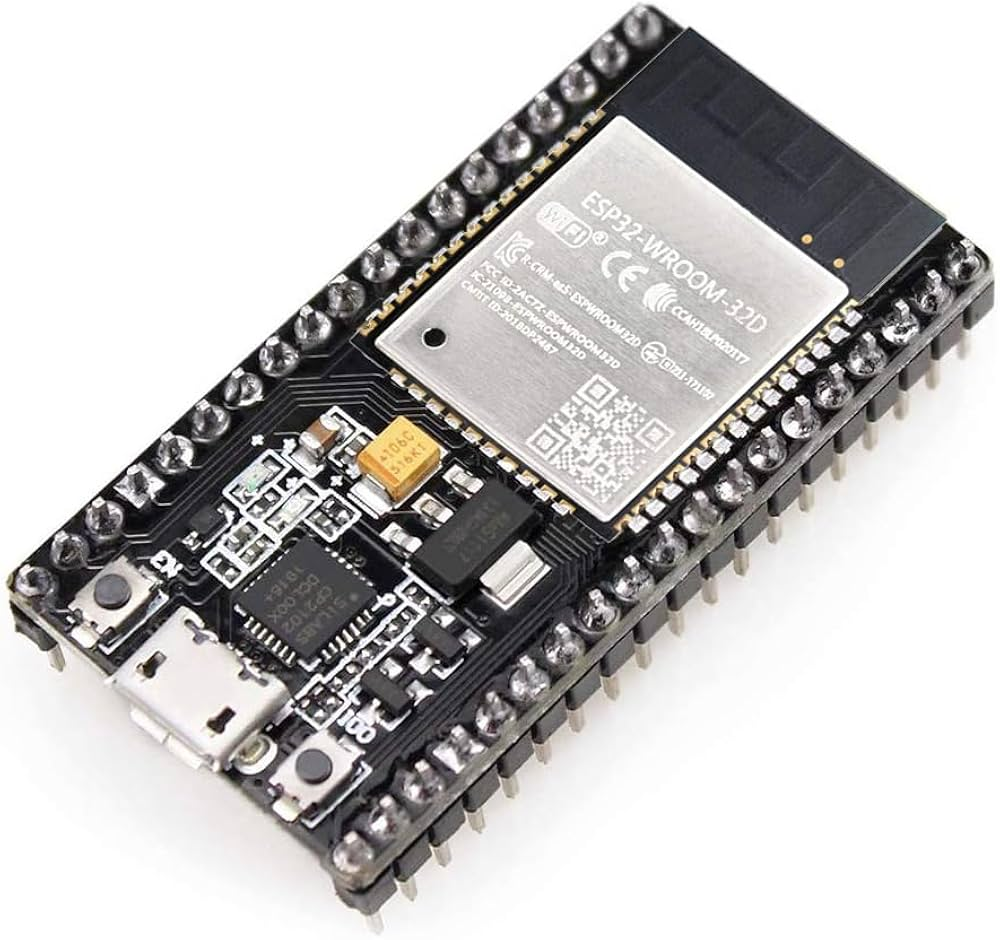
\includegraphics[width=3cm, height=3cm, keepaspectratio]{hw_esp32} &
    \textbf{ESP32-WROOM-32D}\newline
    \textit{Núcleo de procesamiento local del nodo (RF-02, RF-03, RF-04).}\newline
    \textit{Specs}: Dual-core Xtensa LX6 a 240 MHz, Wi-Fi 802.11 b/g/n, Bluetooth v4.2, 520 KB SRAM, 4 MB Flash.\newline
    \textit{Función}: Ejecuta FreeRTOS, controla el motor, gestiona el sensor ultrasónico y mantiene la comunicación TCP/IP de baja latencia con el servidor central. \\
    \midrule
    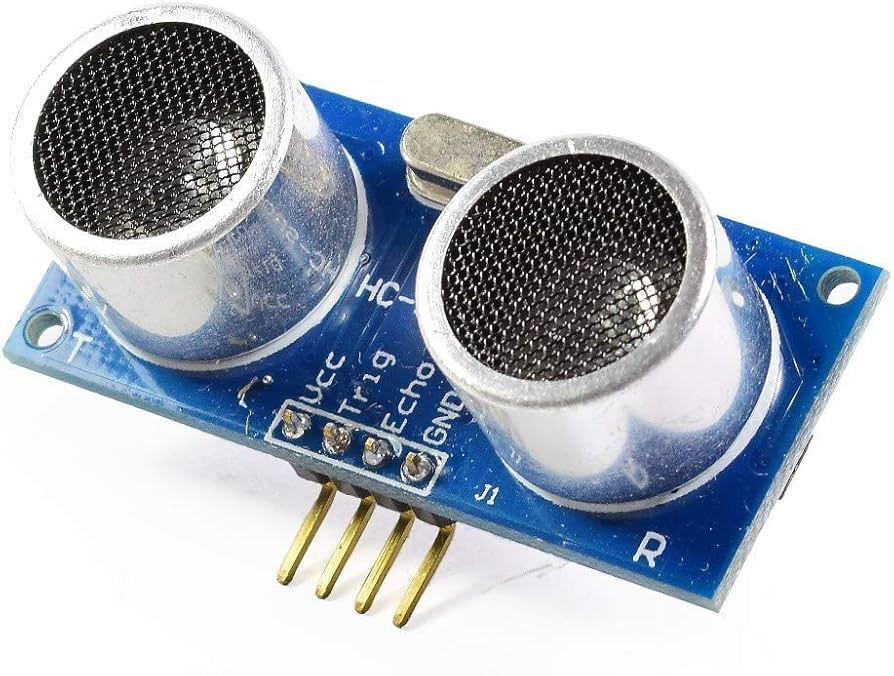
\includegraphics[width=3cm, height=3cm, keepaspectratio]{hw_hcsr04} &
    \textbf{Sensor Ultrasónico HC-SR04}\newline
    \textit{Transductor acústico (RF-01, RF-03).}\newline
    \textit{Specs}: Rango 2 cm -- 400 cm, resolución 3 mm, frecuencia de emisión 40 kHz.\newline
    \textit{Función}: Emite y capta pulsos de sonido para calcular el Tiempo de Vuelo (ToF) y medir distancias espaciales. \\
    \midrule
    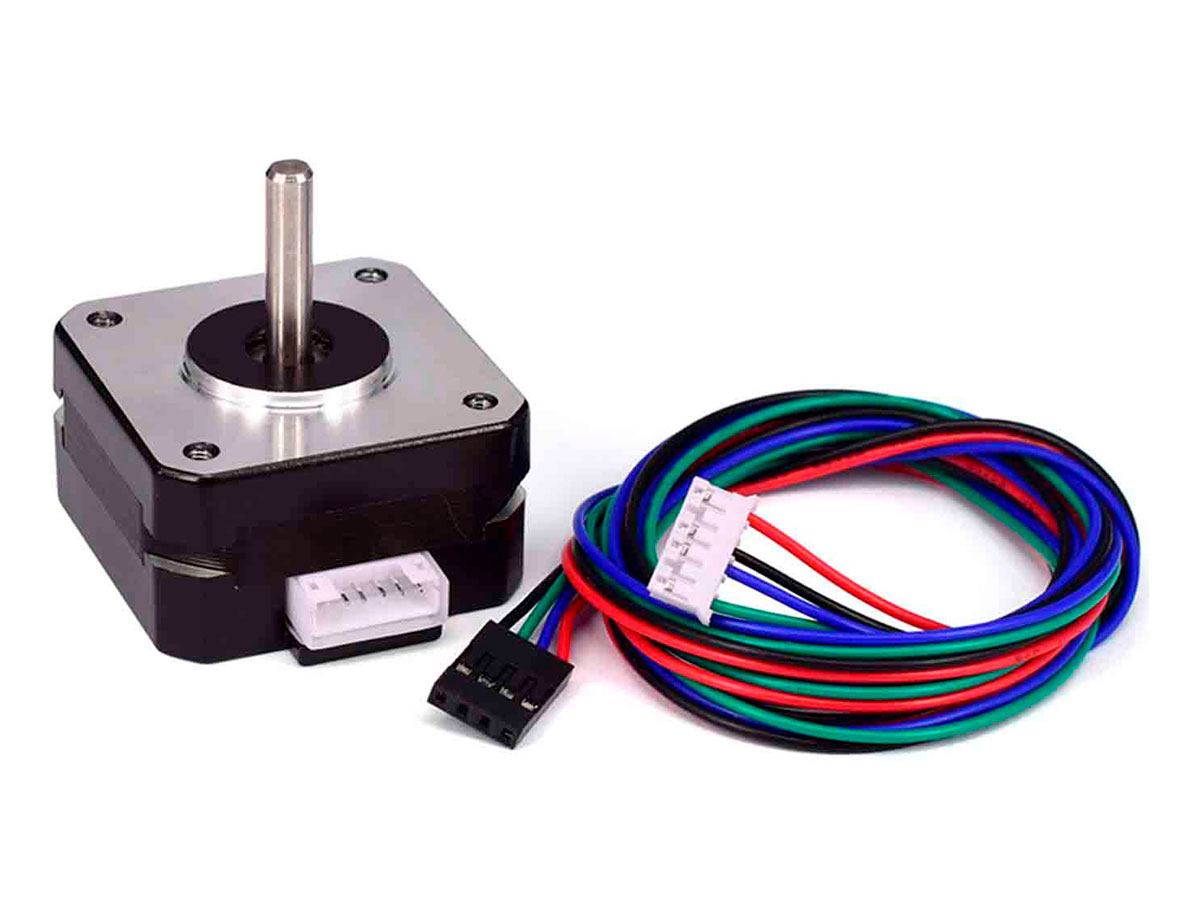
\includegraphics[width=3cm, height=3cm, keepaspectratio]{hw_nema17} &
    \textbf{Motor Paso a Paso NEMA 17}\newline
    \textit{Actuador mecánico (RF-02).}\newline
    \textit{Specs}: Ángulo de paso 1.8° (200 pasos/vuelta), resolución con micropaso 1/16 $\rightarrow$ 3200 pasos/vuelta, alto par de retención.\newline
    \textit{Función}: Ejecuta el barrido perimetral de $360^{\circ}$, orientando el cabezal del sensor con precisión micrométrica. \\
    \midrule
    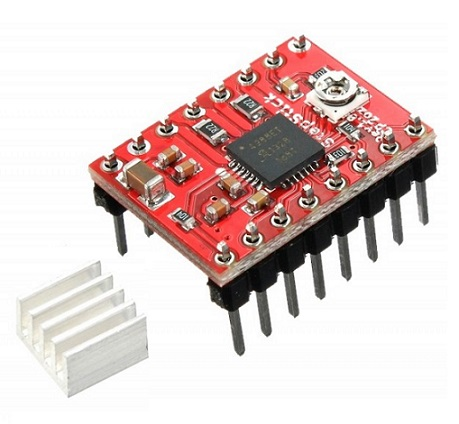
\includegraphics[width=3cm, height=3cm, keepaspectratio]{hw_a4988} &
    \textbf{Driver A4988}\newline
    \textit{Controlador de potencia del motor (RF-02).}\newline
    \textit{Specs}: Soporta hasta 35V / 2A, soporta microstepping hasta 1/16.\newline
    \textit{Función}: Traduce las señales digitales (Step/Dir) del ESP32 en energía para las bobinas del motor. \\
    \midrule
    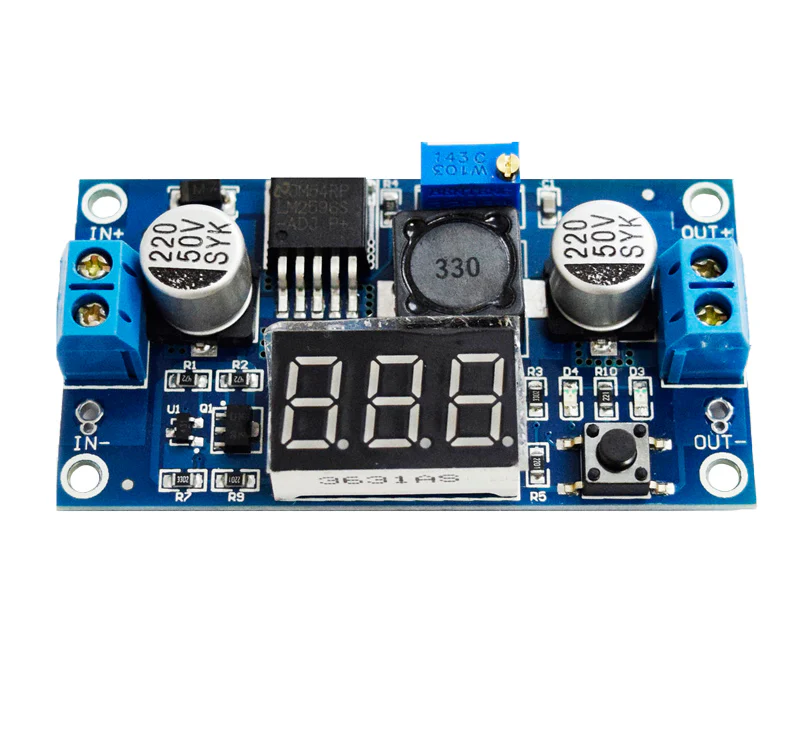
\includegraphics[width=3cm, height=3cm, keepaspectratio]{hw_lm2596} &
    \textbf{Regulador Step-Down LM2596}\newline
    \textit{Conversor de voltaje DC-DC (RNF-01).}\newline
    \textit{Specs}: Entrada hasta 40V, salida estabilizada a 5V (3A máx.).\newline
    \textit{Función}: Reduce y aísla la tensión del bus principal de 24V para alimentar la lógica del ESP32 y el sensor. \\
    \midrule
    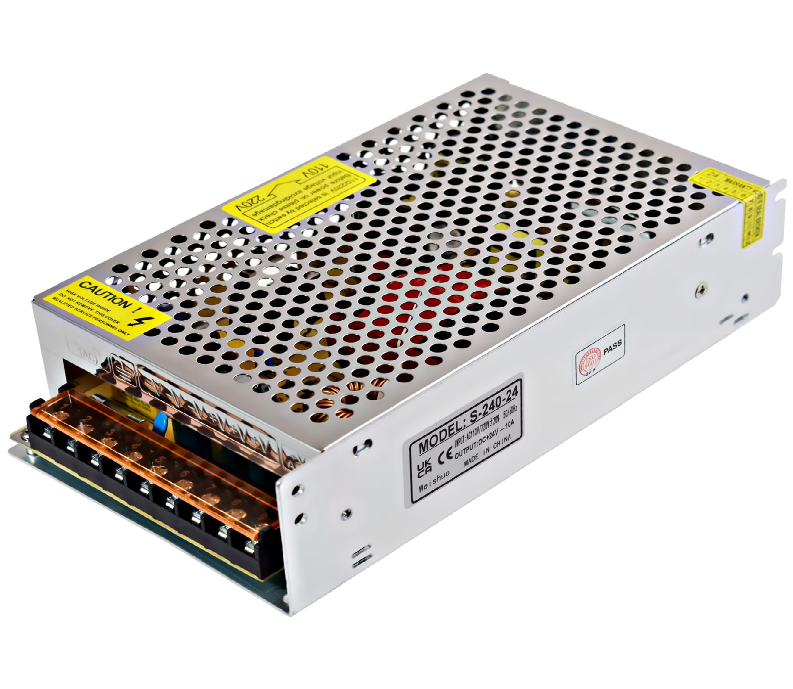
\includegraphics[width=3cm, height=3cm, keepaspectratio]{hw_fuente24v} &
    \textbf{Fuente de Alimentación 24V}\newline
    \textit{Fuente de energía centralizada (RNF-09).}\newline
    \textit{Specs}: Salida de 24V DC, 60W (2{,}5A).\newline
    \textit{Función}: Suministra potencia estable al bus común, alimentando directamente la etapa de potencia de los motores. \\
    \midrule
    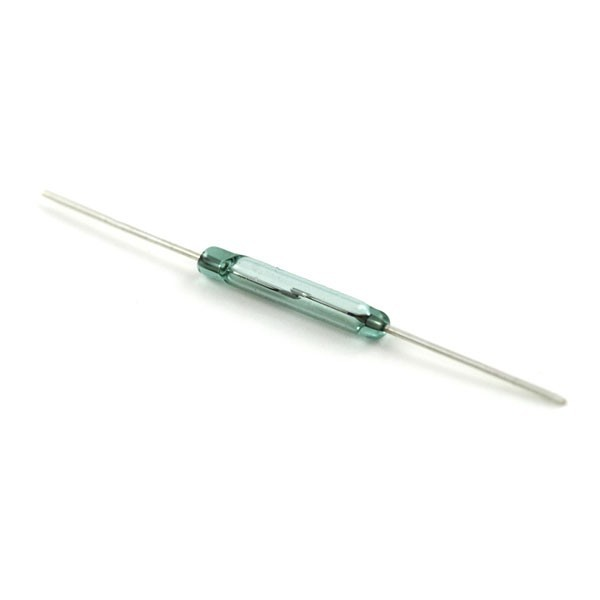
\includegraphics[width=3cm, height=3cm, keepaspectratio]{hw_reed_switch} &
    \textbf{Reed Switch}\newline
    \textit{Interruptor magnético (RF-02).}\newline
    \textit{Función}: Actúa como sensor de fin de carrera para establecer el punto de origen (cero angular) en la calibración inicial del motor. \\
    \bottomrule
\end{tabular}
\vspace{6pt}
\caption{Componentes hardware de cada nodo.}
\label{tab:componentes_hw}
\end{table}

\clearpage
\subsection{Diagrama de conexiones}

La Figura~\ref{fig:diagrama_conexiones} presenta el diagrama de conexiones del nodo sensorial, que integra los periféricos con el microcontrolador ESP32 y establece la infraestructura de potencia.

La gestión de la energía utiliza un convertidor reductor LM2596 que aísla eléctricamente el dominio de potencia del motor paso a paso del dominio lógico del microcontrolador. Esta separación previene que el ruido electromagnético y los picos de corriente generados por el motor causen reinicios del hardware en el ESP32 (RNF-01).

El control del motor se lleva a cabo a través del driver A4988. Sus pines de configuración (MS1, MS2 y MS3) están conectados a la línea de 3.3V para fijar una resolución cinemática de 1/16 de paso. Las señales de control STEP y DIR incluyen resistencias pull-down de 10 k$\Omega$, garantizando un estado lógico definido durante la secuencia de arranque.

El sensor ultrasónico HC-SR04 se alimenta a 5V y conecta su pin ECHO directamente al GPIO del ESP32 para la lectura del retorno del pulso. La calibración mecánica se gestiona mediante el reed switch, que proporciona una señal de interrupción estable durante la rutina de homing.

\begin{figure}[H]
    \centering
    \includegraphics[width=\textwidth]{diagrama_conexiones}
    \caption{Diagrama de conexiones del nodo radar.}
    \label{fig:diagrama_conexiones}
\end{figure}

\subsection{Elementos Estructurales de Soporte en impresión 3D}

El diseño mecánico de las piezas estructurales del nodo radar ha sido creado desde cero a través del modelado paramétrico en 3D. Esta elección permite una personalización completa del ensamblaje, asegurando la fijación precisa de los componentes electrónicos y mecánicos, además de reducir significativamente los costos de producción para la escalabilidad de la red (RNF-09). El modelado se ha llevado a cabo utilizando el software Tinkercad.

El diseño tridimensional del nodo ha sido modularizado para simplificar su impresión, ensamblaje y mantenimiento, lo que permite la sustitución de piezas individuales sin necesidad de reconstruir toda la estructura. Se divide funcionalmente en:

\begin{itemize}[topsep=4pt, partopsep=0pt, itemsep=2pt, parsep=0pt]
    \item \textbf{Chasis (Placas Superior e Inferior):} Base estructural rígida que define el nodo y ancla el resto de los módulos.
    \item \textbf{Soportes de Control (ESP32 y Mini-Protoboard):} Aseguran de manera firme el microcontrolador y la electrónica de potencia.
    \item \textbf{Soportes Electromecánicos (Motor y Reed Switch):} Fijan el motor paso a paso contra la torsión y posicionan el sensor magnético para la calibración inicial (homing).
    \item \textbf{Cabezal Rotatorio (Soporte Sensor HC-SR04):} Se conecta al eje del motor y sostiene el sensor ultrasónico a presión, evitando vibraciones que puedan distorsionar la medición.
    \item \textbf{Elementos Auxiliares:} Piezas menores destinadas a la gestión del cableado interno y al refuerzo entre placas.
\end{itemize}

El diseño estructural del nodo periférico ha sido concebido de manera modular para facilitar su impresión en 3D y su posterior ensamblaje. En la Figura~\ref{fig:nodo_3d_esquema} se muestra el esquema del diseño tridimensional, donde se detallan las diferentes piezas y soportes individuales necesarios para albergar la electrónica y la mecánica del sistema. Una vez que todos estos componentes están integrados, el resultado es un bloque funcional y compacto. Como se ilustra en la Figura~\ref{fig:nodo_3d_cotas}, las vistas de planta y alzado del ensamblaje final presentan las dimensiones generales expresadas en milímetros. Esta representación define el volumen espacial total que ocupa el dispositivo en su entorno operativo, garantizando las tolerancias físicas requeridas entre el microcontrolador ESP32, el motor paso a paso y el sensor ultrasónico.

%\begin{figure}[H]
%    \centering
%    \includegraphics[width=0.75\textwidth]{fig_nodo_3d_esquema}
%    \caption{Esquema del diseño tridimensional.}
%    \label{fig:nodo_3d_esquema}
%\end{figure}

%\begin{figure}[H]
%    \centering
%    \includegraphics[width=0.75\textwidth]{fig_nodo_3d_cotas}
%    \caption{Vistas de planta y alzado del ensamblaje final del nodo periférico con cotas generales (mm).}
%    \label{fig:nodo_3d_cotas}
%\end{figure}

\subsubsection*{Evolución Iterativa del Diseño}

Para lograr el modelo definitivo, la estructura ha sido sometida a un proceso empírico de mejora continua, abordando diversos desafíos mecánicos en cada etapa. Como se muestra en la Figura~\ref{fig:nodo_iteraciones}, el desarrollo atravesó tres diseños preliminares antes de alcanzar el modelo final:

\begin{itemize}[topsep=4pt, partopsep=0pt, itemsep=2pt, parsep=0pt]
    \item \textbf{Iteración 1 (Figura~\ref{fig:nodo_iteraciones}-A):} Enfocada en el diseño general, sin considerar soportes ni compartimentos del hardware. Consistía únicamente en dos placas superpuestas sin ajuste milimétrico ni dimensiones específicas.
    \item \textbf{Iteración 2 (Figura~\ref{fig:nodo_iteraciones}-B):} Rediseño estructural para integrar la electrónica. Se amplió el chasis inferior creando compartimentos para el ESP32 y la protoboard del driver A4988, teniendo en cuenta el espacio necesario para el ruteo del cableado. Se modeló y añadió un soporte lateral específico para el reed switch, esencial para llevar a cabo la rutina de homing mecánico, y se incorporaron orificios en la placa superior para la organización de cables.
    \item \textbf{Iteración 3 (Figura~\ref{fig:nodo_iteraciones}-C):} Rediseño total del soporte del sensor HC-SR04 para optimizar el uso del espacio y ajustarlo para la conexión del imán con el reed switch. También se rediseñó el lugar de sujeción del reed switch, con una apertura más amplia hacia los lados y un agujero en el centro para permitir el paso de cables sin interferir con la mecánica del motor.
\end{itemize}

%\begin{figure}[!ht]
%    \centering
%    \includegraphics[width=\textwidth]{fig_nodo_iteraciones}
%    \caption{Evolución de los prototipos preliminares del nodo: A) Iteración 1, B) Iteración 2 y C) Iteración 3.}
%    \label{fig:nodo_iteraciones}
%\end{figure}

Finalmente, en la Versión Final (Figura~\ref{fig:nodo_final}), se realizó la optimización de los ajustes a presión (\textit{press-fit}) con el objetivo de eliminar cualquier holgura o vibración durante el desplazamiento de todos los compartimentos del hardware, así como el ajuste final de los espacios para el cableado general.

%\begin{figure}[!ht]
%    \centering
%    \includegraphics[width=0.85\textwidth]{fig_nodo_final}
%    \caption{Diseño de la Versión Final del nodo.}
%    \label{fig:nodo_final}
%\end{figure}

% ============================================================
\section{Diseño Software}
% ============================================================

El diseño del software del sistema incluye el servidor central Python y el protocolo de comunicación que lo vincula con los nodos ESP32. Esta sección aborda el sistema desde una perspectiva general hasta llegar a detalles específicos: primero se presenta la arquitectura global, luego la topología de red, a continuación el modelo de datos que establece qué información circula por el sistema, el modelo procedimental que explica cómo se lleva a cabo cada ciclo de medición, y finalmente los modos de operación que definen el comportamiento del sistema en tiempo real.

\subsection{Visión General de la Arquitectura}

El sistema se estructura en cinco capas funcionales que delimitan las responsabilidades de cada uno de sus componentes. En la base se encuentra el hardware físico de los nodos; encima de este, el firmware que lo gestiona; luego, la capa de comunicaciones; posteriormente, el servidor central que toma las decisiones; y en la parte superior, la interfaz gráfica que presenta los resultados. Esta jerarquía asegura que cada capa dependa únicamente de la inmediatamente inferior, lo que facilita el mantenimiento y permite la sustitución de componentes sin impactar en el resto. La Figura~\ref{fig:arquitectura_capas} ilustra esta estructura.

\begin{itemize}[topsep=4pt, partopsep=0pt, itemsep=2pt, parsep=0pt]
    \item \textbf{Capa 1: Capa Física y de Hardware:} Constituye la base electromecánica, compuesta por los elementos físicos de cada nodo: el SoC ESP32-WROOM-32D, el sensor ultrasónico HC-SR04, el motor paso a paso NEMA 17 junto con su driver A4988 y el sensor reed para la calibración mecánica. La utilización de hardware comercial de bajo costo asegura la escalabilidad de la red (RNF-03, RNF-09).
    \item \textbf{Capa 2: Capa de Abstracción de Hardware (HAL):} Representa la capa de abstracción de hardware (HAL), que opera en el Core 1 del microcontrolador y aísla la lógica de control de los aspectos eléctricos de los periféricos, gestionando de manera determinista las interrupciones del sensor y los pulsos del motor (RF-02, RF-03).
    \item \textbf{Capa 3: Capa de Comunicaciones y Enlace:} Se encarga de las comunicaciones entre los nodos y el servidor: implementa la pila TCP/IP, el protocolo binario y la supertrama TDMA que coordina el acceso al medio acústico sin interferencias (RF-01, RF-04).
    \item \textbf{Capa 4: Capa de Orquestación y Procesamiento Lógico:} Es el servidor central desarrollado en Python, que centraliza la inteligencia del sistema: procesa la telemetría a través de trilateración, gestiona el cambio entre modos de operación y resuelve los conflictos en las áreas de solapamiento (RF-06, RF-08).
    \item \textbf{Capa 5: Capa de Presentación e Interfaz de Usuario (HMI):} Es la interfaz gráfica, que presenta el entorno mapeado en un lienzo 2D y ofrece al operador paneles de control y consolas de depuración para gestionar la red (RF-07).
\end{itemize}

%\begin{figure}[H]
%    \centering
%    \includegraphics[width=0.85\textwidth]{fig_arquitectura_capas}
%    \caption{Diagrama de la estructura por capas del sistema.}
%    \label{fig:arquitectura_capas}
%\end{figure}

El servidor central constituye el elemento más intrincado del software. La Figura~\ref{fig:flujo_servidor} ilustra su ciclo de vida integral, desde el inicio hasta el bucle continuo de la supertrama. Al comenzar, el servidor registra su dirección en la red a través de mDNS y abre el puerto TCP 8080 para recibir conexiones de los nodos; simultáneamente, inicia un hilo de orquestación y un hilo manejador por cada nodo que se conecte. Una vez que al menos un nodo está conectado, el servidor se adentra en el bucle de supertrama que se repite de manera indefinida: emite el pulso de sincronización, recoge las propuestas de ángulo, calcula las asignaciones de slot, espera a que los nodos realicen las mediciones, recoge los resultados, actualiza el estado del sistema y envía los datos al visualizador. Cada una de las etapas de este bucle se detalla minuciosamente en el punto 5.2.4.

%\begin{figure}[H]
%    \centering
%    \includegraphics[width=0.75\textwidth]{fig_flujo_servidor}
%    \caption{Diagrama de flujo del bucle de orquestación del servidor central.}
%    \label{fig:flujo_servidor}
%\end{figure}

\subsection{Topología de Red y Distribución Física}

Para que los tres nodos ESP32 y el servidor central puedan coordinarse en tiempo real, el sistema requiere una infraestructura de red que satisfaga tres condiciones: que los mensajes sean recibidos en orden y sin pérdidas, que la latencia sea lo suficientemente baja para no afectar la sincronización temporal del protocolo TDMA, y que los nodos tengan la capacidad de localizar al servidor de manera automática sin necesidad de configuración manual. Esta sección detalla cómo se abordan estas tres condiciones mediante la topología de red adoptada, el mecanismo de descubrimiento automático del servidor y la disposición física de los nodos en el área de vigilancia.

\subsubsection*{Modelo Cliente-Servidor en Estrella}

La red del sistema adopta una topología en estrella con un modelo cliente-servidor, donde el servidor actúa como el único nodo maestro y los tres ESP32 funcionan como clientes periféricos. Como se ilustra en la Figura~\ref{fig:topologia_estrella}, ningún nodo se comunica directamente con otro; toda la coordinación se realiza a través del servidor. Esta elección se fundamenta en que el algoritmo de orquestación necesita conocer el estado de todos los nodos de manera simultánea antes de tomar cualquier decisión: asignar slots, detectar conflictos y calcular posiciones son operaciones que requieren una visión global que solo posee el servidor. Una topología distribuida o en malla implicaría un protocolo de consenso entre nodos, lo que añadiría latencia de sincronización y complejidad de implementación que son incompatibles con los requisitos temporales del sistema.

La comunicación emplea TCP con conexiones persistentes, en lugar de establecer una conexión por cada mensaje. Esto implica que, una vez que el nodo se conecta al servidor, el socket se mantiene abierto durante toda la sesión operativa. Esta elección conlleva tres consecuencias directas: el servidor puede detectar la caída de un nodo de inmediato al cerrarse el socket, sin requerir paquetes de keepalive explícitos; se elimina el costo de establecimiento de conexión (SYN/SYN-ACK/ACK) en cada ciclo, lo que en una red WiFi doméstica puede superar los 10 ms; y el estado de la conexión queda completamente delegado en la pila TCP del sistema operativo, lo que simplifica el firmware del nodo.

Para disminuir la latencia dentro de la conexión persistente, el sistema desactiva el algoritmo de Nagle en todos los sockets TCP y el modo de ahorro de energía del módulo WiFi del ESP32. El algoritmo de Nagle acumula pequeños datos en un búfer antes de enviarlos para mejorar la eficiencia de la red, lo cual es adecuado para transferencias de archivos, pero resulta contraproducente en este caso: con mensajes que oscilan entre 0 y 13 bytes de carga útil y un ciclo de supertrama que depende de que cada mensaje llegue en el momento preciso, un retraso artificial de hasta 200 ms podría desincronizar las mediciones. El modo de ahorro de energía del WiFi introduce retardos similares al poner el módulo en modo de bajo consumo entre transmisiones.

%\begin{figure}[H]
%    \centering
%    \includegraphics[width=0.75\textwidth]{fig_topologia_estrella}
%    \caption{Representación lógica del modelo cliente-servidor en estrella.}
%    \label{fig:topologia_estrella}
%\end{figure}

\subsubsection*{Descubrimiento Automático del Servidor}

Para que los nodos puedan localizar el servidor sin la necesidad de establecer direcciones IP estáticas, el sistema recurre a mDNS (\textit{Multicast DNS}). Al iniciar, el servidor registra su dirección bajo el nombre de host \texttt{radar-server.local} utilizando la biblioteca \texttt{zeroconf}, que publica un registro de servicio del tipo \texttt{radar.\_tcp.local} con todas las interfaces de red activas del servidor. Este mecanismo permite implementar el sistema en cualquier red local sin necesidad de modificar el firmware ni el servidor, dado que la resolución de nombres se realiza de manera automática.

La Figura~\ref{fig:descubrimiento_mdns} representa el proceso integral de descubrimiento que lleva a cabo el nodo al establecer conexión con WiFi. En primer lugar, intenta resolver \texttt{radar-server.local} a través de mDNS; si no obtiene respuesta en dos intentos consecutivos ---lo cual puede suceder en redes donde el tráfico multicast está restringido---, el nodo opta por utilizar la IP del gateway como alternativa. Este modo de respaldo es efectivo porque, en el entorno de despliegue habitual, el servidor se encuentra en la misma máquina que actúa como punto de acceso, lo que implica que el gateway y el servidor comparten la misma dirección IP. Una vez que la dirección es resuelta, se almacena en caché para que las reconexiones futuras puedan utilizarla directamente sin necesidad de realizar una nueva resolución mDNS.

El firmware también permite la configuración de múltiples redes WiFi de manera simultánea. Al iniciar, el nodo realiza un escaneo activo de las SSIDs disponibles y se conecta a la primera que coincida con alguna de las redes configuradas, siguiendo el orden de preferencia establecido en \texttt{Config.h}. Esta funcionalidad facilita el despliegue del mismo firmware en laboratorio, en el hogar o en el campo sin necesidad de recompilación, lo que acelera el ciclo de desarrollo y pruebas.

%\begin{figure}[H]
%    \centering
%    \includegraphics[width=0.75\textwidth]{fig_descubrimiento_mdns}
%    \caption{Diagrama de flujo del descubrimiento automático del servidor.}
%    \label{fig:descubrimiento_mdns}
%\end{figure}

\subsubsection*{Disposición Física y Zonas de Cobertura}

La disposición física de los nodos en el espacio no es aleatoria: influye directamente en la precisión del sistema y en las condiciones bajo las cuales se presenta la interferencia acústica. Los tres nodos se encuentran ubicados en el perímetro del área de vigilancia formando un triángulo, y cada uno tiene asignado un ángulo de orientación $\theta$ configurado en \texttt{grid\_config.json} que dirige su eje frontal hacia el interior del área. La Figura~\ref{fig:distribucion_fisica} representa esta configuración y los efectos geométricos que genera.

Cada sensor opera dentro de un rango angular de $\pm 45^{\circ}$ en relación a su eje frontal, lo que proporciona a cada nodo un campo de visión efectivo de $90^{\circ}$. Dado que los nodos están orientados hacia el mismo espacio interior, los campos de visión de los pares adyacentes N1-N2 y N2-N3 se superponen parcialmente en los extremos de ese rango. Esta superposición da lugar a lo que el sistema denomina \textit{zona sucia}: la región angular donde un nodo, al apuntar hacia el extremo de su campo de visión, puede estar dirigiéndose en la misma dirección que el nodo vecino. El umbral que define la zona sucia está establecido en $\pm 30^{\circ}$ de ángulo local; más allá de este valor, el nodo se considera en zona sucia y susceptible de causar interferencia con su vecino.

Este solapamiento geométrico tiene dos consecuencias opuestas. Por un lado, es la causa del problema de interferencia acústica que el protocolo TDMA soluciona mediante la asignación de intervalos temporales. Por otro lado, representa una ventaja para la estimación de posición: cuando dos nodos detectan simultáneamente el mismo objetivo en zona sucia, el servidor cuenta con dos mediciones independientes del mismo punto y puede combinarlas para obtener una estimación más sólida de las coordenadas globales, tal como se detalla en el punto 5.2.5.

%\begin{figure}[H]
%    \centering
%    \includegraphics[width=0.85\textwidth]{fig_distribucion_fisica}
%    \caption{Abstracción geométrica de la distribución perimetral, orientaciones acústicas y áreas de intersección (\textit{crosstalk}).}
%    \label{fig:distribucion_fisica}
%\end{figure}

% ============================================================
\subsection{Modelo de Datos: Módulos del Sistema}
% ============================================================

El sistema se organiza en dos componentes de software independientes: el servidor central, implementado como una única clase Python que centraliza toda la lógica de orquestación, y el firmware del nodo ESP32, distribuido en cuatro módulos C++ que siguen la arquitectura por capas descrita en la sección 5.2.1. Esta sección documenta la estructura interna de ambos componentes: sus variables de estado, sus métodos y los archivos de persistencia que mantienen la información entre sesiones.

\subsubsection*{Servidor central: clase \texttt{ArbitroServer}}

El servidor central se implementa íntegramente en el archivo \texttt{server\_central.py} como una única clase Python, \texttt{ArbitroServer}, que concentra toda la inteligencia del árbitro. Para clarificar su organización interna, el diagrama UML de la Figura~\ref{fig:uml_servidor} descompone la clase en cuatro agrupaciones funcionales: el \textbf{estado central compartido}, el \textbf{orquestador de supertramas}, el \textbf{localizador cooperativo} y el \textbf{gestor de persistencia}. Aunque en el código todas estas responsabilidades residen en la misma clase, la separación conceptual facilita la comprensión de sus mecanismos internos y la futura extensión del sistema.

El \textbf{estado central} agrupa los atributos de instancia accesibles de forma simultánea desde el hilo de aceptación de conexiones y los hilos individuales de cada nodo. Comprende los registros de clientes activos (\texttt{clients}, \texttt{client\_sockets}), los búferes de recepción TCP por socket (\texttt{client\_buffers}), los diccionarios de estado operativo (\texttt{track\_states}, \texttt{latest\_reports}, \texttt{reports\_received}), los contadores de tolerancia (\texttt{strikes}, \texttt{grace\_until\_sf}, \texttt{track\_lock}) y las variables de progreso del ciclo (\texttt{seq}, \texttt{current\_phase}, \texttt{running}). El acceso concurrente a este estado se serializa mediante \texttt{lock}, un \texttt{threading.Lock} que garantiza la coherencia de las escrituras entre múltiples hilos.

El \textbf{orquestador de supertramas} encapsula la lógica temporal del sistema. Su método central, \texttt{orchestration\_loop()}, ejecuta de forma continua las seis fases del ciclo TDMA descritas en el apartado~5.2.4, guiado por las constantes de módulo \texttt{DIRTY\_MARGIN}, \texttt{MAX\_MISSES} y \texttt{TRACK\_LOCK\_DURATION} para parametrizar la detección de conflictos de zona sucia y la gestión del modo TRACK. El método auxiliar \texttt{calculate\_movement\_time()} estima el tiempo de desplazamiento del motor entre dos ángulos ---a partir del paso angular, el microstepping y la relación de transmisión--- y proporciona el valor del retardo temporal incluido en cada \texttt{MSG\_SLOT\_ASSIGN}.

El \textbf{localizador cooperativo} agrupa los métodos de procesamiento geométrico. \texttt{calculate\_global\_coords()} transforma la medición polar local de un nodo (ángulo y distancia) a coordenadas cartesianas del plano global de vigilancia, aplicando la orientación $\theta$ del nodo almacenada en \texttt{grid}. \texttt{calcular\_trilateracion()} combina las observaciones polares independientes de dos nodos adyacentes para estimar la posición de un obstáculo compartido mediante intersección de circunferencias, mecanismo que se detalla en el apartado~5.2.5.

El \textbf{gestor de persistencia} encapsula la interfaz con los archivos JSON de sesión. Las variables de ruta \texttt{CONFIG\_FILE} y \texttt{STATE\_FILE} centralizan las referencias a disco; los métodos \texttt{load\_grid()} y \texttt{save\_grid()} gestionan la configuración topológica de los nodos, mientras que \texttt{load\_state()}, \texttt{save\_state()} y \texttt{\_save\_state\_silent()} mantienen el estado operativo entre sesiones. La estructura de ambos archivos se documenta en el subapartado siguiente. La Tabla~\ref{tab:modulo_arbitro} recoge la especificación completa de todas las variables y métodos de la clase.

% Sube a figuras/: fig_uml_servidor.png
%\begin{figure}[H]
%    \centering
%    \includegraphics[width=\textwidth]{fig_uml_servidor}
%    \caption{Diagrama de clases UML del servidor central (\texttt{server\_central.py}).}
%    \label{fig:uml_servidor}
%\end{figure}

\begin{table}[H]
\centering
\resizebox{\textwidth}{!}{%
\begin{tabular}{|p{5cm}|p{9.5cm}|p{4cm}|p{3cm}|}
\hline
\multicolumn{4}{|c|}{\textbf{Módulo \texttt{ArbitroServer} --- \texttt{server\_central.py}}} \\
\hline
\multicolumn{4}{|p{21.5cm}|}{Implementa la lógica completa del servidor central. Gestiona las conexiones TCP de los nodos mediante hilos concurrentes, ejecuta el bucle de la supertrama TDMA, administra el estado SEARCH/TRACK de cada nodo, resuelve los conflictos de zona sucia mediante arbitraje de bloqueo temporal y emite el estado del sistema al visualizador mediante UDP.} \\
\hline
\multicolumn{4}{|c|}{\textbf{Tabla de variables}} \\
\hline
\textbf{Nombre} & \textbf{Descripción} & \multicolumn{2}{c|}{\textbf{Tipo de dato}} \\
\hline
\texttt{clients} & Mapeo de socket activo al identificador numérico de nodo. & \multicolumn{2}{l|}{\texttt{dict[socket, int]}} \\
\hline
\texttt{client\_sockets} & Acceso inverso: de identificador de nodo a su socket, utilizado para el envío dirigido de mensajes. & \multicolumn{2}{l|}{\texttt{dict[int, socket]}} \\
\hline
\texttt{track\_states} & Estado operativo completo por nodo: modo SEARCH/TRACK, contadores \texttt{misses} y \texttt{edge\_flips}, dirección de barrido y ángulo actual. & \multicolumn{2}{l|}{\texttt{dict[int, dict]}} \\
\hline
\texttt{grid} & Configuración física de los nodos (posición, orientación $\theta$, dirección MAC). Cargado desde \texttt{grid\_config.json} al inicio. & \multicolumn{2}{l|}{\texttt{dict}} \\
\hline
\texttt{strikes} & Contador de superframes consecutivos sin respuesta válida por nodo. Al alcanzar 7 strikes el servidor cierra la conexión. & \multicolumn{2}{l|}{\texttt{dict[int, int]}} \\
\hline
\texttt{grace\_until\_sf} & Número de superframe hasta el cual un nodo recién conectado no acumula strikes. & \multicolumn{2}{l|}{\texttt{dict[int, int]}} \\
\hline
\texttt{track\_lock} & Número de superframe hasta el cual el nodo ganador de un conflicto mantiene inmunidad de TRACK. & \multicolumn{2}{l|}{\texttt{dict[int, int]}} \\
\hline
\texttt{seq} & Número de secuencia del superframe en curso, incrementado al final de cada ciclo. & \multicolumn{2}{l|}{\texttt{int}} \\
\hline
\texttt{lock} & Mutex que serializa el acceso concurrente al estado compartido desde los hilos de cliente y el hilo de orquestación. & \multicolumn{2}{l|}{\texttt{threading.Lock}} \\
\hline
\texttt{udp\_sock} & Socket UDP para emitir el estado completo del sistema al visualizador en el puerto 8081 al final de cada superframe. & \multicolumn{2}{l|}{\texttt{socket.socket}} \\
\hline
\texttt{client\_buffers} & Búfer de recepción TCP por conexión, necesario para parsear tramas de longitud variable sobre un flujo de bytes continuo. & \multicolumn{2}{l|}{\texttt{dict[socket, bytes]}} \\
\hline
\texttt{defcon1\_limit \ldots valla\_limit} & Umbrales de distancia en cm que delimitan las zonas de criticidad, recargados desde \texttt{visualizer\_settings.json} en cada ciclo. & \multicolumn{2}{l|}{\texttt{float}} \\
\hline
\multicolumn{4}{|c|}{\textbf{Tabla de métodos}} \\
\hline
\textbf{Nombre} & \textbf{Descripción} & \textbf{Dato(s) de entrada} & \textbf{Dato(s) de salida} \\
\hline
\texttt{\_\_init\_\_()} & Constructor. Inicializa todas las estructuras de estado, carga la configuración de red y el estado de la sesión anterior, y abre el socket UDP. & Ninguno & Ninguno \\
\hline
\texttt{load\_grid()} & Lee \texttt{grid\_config.json} y devuelve el diccionario de configuración física de nodos. & Ninguno & \texttt{dict} \\
\hline
\texttt{save\_grid()} & Persiste el diccionario \texttt{grid} en \texttt{grid\_config.json}. & Ninguno & Ninguno \\
\hline
\texttt{load\_state()} & Carga \texttt{radar\_state.json} tras confirmación interactiva. Devuelve el diccionario de estados o un diccionario vacío si el usuario rechaza la sesión anterior. & Ninguno & \texttt{dict} \\
\hline
\texttt{save\_state()} & Escribe \texttt{track\_states} en \texttt{radar\_state.json} con mensaje de confirmación por consola. Se invoca al detener el servidor. & Ninguno & Ninguno \\
\hline
\texttt{\_save\_state\_silent()} & Guardado periódico silencioso del estado, ejecutado cada 15 superframes sin interrumpir la salida de consola. & Ninguno & Ninguno \\
\hline
\texttt{calculate\_global\_coords()} & Convierte la medición polar local de un nodo (ángulo y distancia) a coordenadas cartesianas del plano global de vigilancia. & \texttt{radar\_id, local\_angle, distance} & \texttt{tuple(x,y)} ó \texttt{None} \\
\hline
\texttt{calcular\_trilateracion()} & Calcula la posición de un objeto por intersección geométrica de dos circunferencias centradas en los nodos del par activo. & \texttt{id1, d1, id2, d2} & \texttt{tuple(x,y)} ó \texttt{None} \\
\hline
\texttt{calculate\_movement\_time()} & Estima el tiempo de desplazamiento del motor entre dos ángulos en milisegundos, a partir de los parámetros cinemáticos del sistema. & \texttt{current\_angle, target\_angle} & \texttt{int} \\
\hline
\texttt{get\_state()} & Devuelve el diccionario de estado de un nodo, inicializando sus campos con valores predeterminados si aún no existe registro para ese nodo. & \texttt{r\_id} & \texttt{dict} \\
\hline
\texttt{remove\_client()} & Elimina todos los registros asociados a un nodo desconectado y cierra su socket. & \texttt{conn, r\_id} & Ninguno \\
\hline
\texttt{handle\_client()} & Hilo manejador de la conexión TCP de un nodo: parsea las tramas entrantes y despacha las acciones correspondientes a cada opcode del protocolo. & \texttt{conn, addr} & Ninguno \\
\hline
\texttt{orchestration\_loop()} & Bucle principal de la supertrama TDMA: ejecuta secuencialmente las seis fases de cada ciclo de medición y coordina todos los nodos activos. & Ninguno & Ninguno \\
\hline
\texttt{start()} & Punto de entrada del servidor: registra el servicio mDNS, abre el puerto TCP 8080, lanza el hilo de orquestación y entra en el bucle de aceptación de conexiones. & Ninguno & Ninguno \\
\hline
\end{tabular}
}
\caption{Descripción del módulo \texttt{ArbitroServer} (\texttt{server\_central.py}).}
\label{tab:modulo_arbitro}
\end{table}

\subsubsection*{Archivos de configuración y persistencia}

El servidor mantiene el estado del sistema en dos archivos JSON. \texttt{grid\_config.json} almacena la configuración topológica de la red y se actualiza automáticamente cuando un nodo desconocido se conecta por primera vez. \texttt{radar\_state.json} persiste el estado operativo de cada nodo entre sesiones, permitiendo reanudar el barrido en el ángulo donde quedó sin necesidad de un homing completo (RF-02). Las Tablas~\ref{tab:json_grid} y~\ref{tab:json_state} describen sus campos.

\begin{table}[H]
\centering
\resizebox{\textwidth}{!}{%
\begin{tabular}{|p{4cm}|p{11cm}|p{2.5cm}|}
\hline
\multicolumn{3}{|c|}{\textbf{Archivo \texttt{grid\_config.json}}} \\
\hline
\multicolumn{3}{|p{17.5cm}|}{Diccionario indexado por la dirección MAC de cada nodo. Almacena la posición física y la orientación de cada radar en el plano de vigilancia. Se crea automáticamente con valores predeterminados cuando un nodo desconocido se conecta por primera vez; el administrador puede editarlo manualmente para ajustar las coordenadas.} \\
\hline
\textbf{Campo} & \textbf{Descripción} & \textbf{Tipo} \\
\hline
\texttt{"XX:XX:XX:XX:XX:XX"} (clave) & Dirección MAC del nodo. Actúa como identificador único persistente entre sesiones. & \texttt{string} \\
\hline
\texttt{id} & Identificador numérico asignado al nodo (1, 2 o 3). & \texttt{int} \\
\hline
\texttt{x}, \texttt{y} & Coordenadas cartesianas de la posición física del nodo en el plano de vigilancia, en centímetros. & \texttt{float} \\
\hline
\texttt{theta} & Ángulo de orientación frontal del nodo en grados, medido desde el eje X positivo. Determina hacia dónde apunta el eje de barrido $0^{\circ}$ del nodo. & \texttt{float} \\
\hline
\end{tabular}
}
\vspace{6pt}
\caption{Estructura del archivo de configuración \texttt{grid\_config.json}.}
\label{tab:json_grid}
\end{table}

\begin{table}[H]
\centering
\resizebox{\textwidth}{!}{%
\begin{tabular}{|p{4cm}|p{11cm}|p{2.5cm}|}
\hline
\multicolumn{3}{|c|}{\textbf{Archivo \texttt{radar\_state.json}}} \\
\hline
\multicolumn{3}{|p{17.5cm}|}{Diccionario indexado por el identificador numérico de cada nodo. Persiste el estado operativo entre sesiones para evitar el homing completo en cada reconexión. Al arrancar, el servidor propone al administrador reutilizar este archivo; si la propuesta se rechaza, el archivo se elimina y todos los nodos comienzan desde $0^{\circ}$.} \\
\hline
\textbf{Campo} & \textbf{Descripción} & \textbf{Tipo} \\
\hline
\texttt{"1"}, \texttt{"2"}, \texttt{"3"} (clave) & Identificador numérico del nodo, almacenado como cadena de texto. & \texttt{string} \\
\hline
\texttt{mode} & Modo operativo activo al terminar la sesión: \texttt{"SEARCH"} o \texttt{"TRACK"}. & \texttt{string} \\
\hline
\texttt{search\_dir} & Dirección de barrido en modo SEARCH al terminar la sesión: \texttt{+1.0} (creciente) o \texttt{-1.0} (decreciente). & \texttt{float} \\
\hline
\texttt{track\_dir} & Dirección de barrido en modo TRACK al terminar la sesión: \texttt{+1.0} (creciente) o \texttt{-1.0} (decreciente). & \texttt{float} \\
\hline
\texttt{misses} & Número de ecos consecutivos no recibidos en modo TRACK al finalizar la sesión. & \texttt{int} \\
\hline
\texttt{edge\_flips} & Número de inversiones de dirección por borde de objeto en modo TRACK al finalizar la sesión. & \texttt{int} \\
\hline
\texttt{track\_entry\_sf} & Superframe en que el nodo entró en TRACK por primera vez en la sesión. Valor centinela $10^{9}$ si no ha habido ninguna detección. & \texttt{int} \\
\hline
\texttt{current\_angle} & Ángulo físico del motor al finalizar la sesión, en grados. Utilizado para reanudar el barrido sin homing. & \texttt{float} \\
\hline
\end{tabular}
}
\vspace{6pt}
\caption{Estructura del archivo de persistencia \texttt{radar\_state.json}.}
\label{tab:json_state}
\end{table}

\subsubsection*{Firmware del nodo ESP32}

% Sube a figuras/: fig_uml_nodo.png
%\begin{figure}[H]
%    \centering
%    \includegraphics[width=\textwidth]{fig_uml_nodo}
%    \caption{Diagrama de clases UML del firmware del nodo ESP32.}
%    \label{fig:uml_nodo}
%\end{figure}

El firmware del nodo se distribuye en cuatro módulos C++ con responsabilidades delimitadas según la arquitectura por capas de la sección~5.2.1, cuyas relaciones se sintetizan en el diagrama de clases UML de la Figura~\ref{fig:uml_nodo}. El archivo \texttt{comms\_protocol.h} define las estructuras binarias del protocolo compartido con el servidor; \texttt{config.h} centraliza las constantes hardware del nodo; la clase \texttt{SystemManager} (declarada en \texttt{system.h}) actúa como repositorio global del estado compartido entre tareas; y las tareas FreeRTOS \texttt{TaskComms} y \texttt{TaskRadar} implementan, respectivamente, la capa de comunicaciones en el Core~0 y la capa de abstracción de hardware en el Core~1.

\subsubsection*{Módulo \texttt{comms\_protocol.h}}

Define exclusivamente los tipos de datos del protocolo TCP: las siete constantes \textit{OpCode} y los ocho \textit{structs} con alineamiento forzado a un byte mediante \texttt{\#pragma pack(push,~1)}. La directiva de empaquetado garantiza que el \textit{cast} directo de un búfer de red sobre la estructura sea seguro y tenga coste computacional nulo. No contiene lógica ejecutable. La Tabla~\ref{tab:modulo_protocol} detalla sus definiciones.

\begin{table}[H]
\centering
\resizebox{\textwidth}{!}{%
\begin{tabular}{|p{5cm}|p{9.5cm}|p{4cm}|p{3cm}|}
\hline
\multicolumn{4}{|c|}{\textbf{Módulo \texttt{comms\_protocol.h}}} \\
\hline
\multicolumn{4}{|p{21.5cm}|}{Define las constantes \textit{OpCode} del protocolo binario y las estructuras \textit{packed} de cada mensaje. Actúa como contrato de interoperabilidad entre el firmware del nodo y el servidor central; cualquier cambio en estas definiciones debe reflejarse simultáneamente en ambos extremos.} \\
\hline
\multicolumn{4}{|c|}{\textbf{Tabla de variables}} \\
\hline
\textbf{Nombre} & \textbf{Descripción} & \multicolumn{2}{c|}{\textbf{Tipo de dato}} \\
\hline
\texttt{MSG\_HELLO\_REQ \ldots MSG\_DATA\_REPORT} & Siete constantes \textit{OpCode} (0xA0--0xD0) que identifican cada tipo de mensaje del protocolo. & \multicolumn{2}{l|}{\texttt{\#define (uint8\_t)}} \\
\hline
\texttt{PacketHeader} & Cabecera de tres bytes presente en todo mensaje: \texttt{type} (OpCode) y \texttt{length} (longitud del payload en little-endian). & \multicolumn{2}{l|}{\texttt{struct (3 B)}} \\
\hline
\texttt{Payload\_HelloReq} & Payload de registro inicial: dirección MAC del nodo en seis octetos consecutivos. & \multicolumn{2}{l|}{\texttt{struct (6 B)}} \\
\hline
\texttt{Payload\_HelloAck} & Payload de confirmación de registro: identificador numérico asignado y ángulo guardado de la sesión anterior. & \multicolumn{2}{l|}{\texttt{struct (5 B)}} \\
\hline
\texttt{Payload\_SuperFrame} & Payload del pulso de sincronización global: número de secuencia y tiempo del servidor en milisegundos. & \multicolumn{2}{l|}{\texttt{struct (8 B)}} \\
\hline
\texttt{Payload\_AngleReq} & Payload de propuesta de ángulo: identificador de nodo, ángulo actual y ángulo propuesto para el siguiente ciclo. & \multicolumn{2}{l|}{\texttt{struct (9 B)}} \\
\hline
\texttt{Payload\_SlotAssign} & Payload de asignación de ranura temporal: identificador de nodo, índice de ranura, retardo desde $t_0$ y ángulo confirmado. & \multicolumn{2}{l|}{\texttt{struct (10 B)}} \\
\hline
\texttt{Payload\_DataReport} & Payload de telemetría: identificador de nodo, ángulo de medición, distancia en centímetros y marca temporal. & \multicolumn{2}{l|}{\texttt{struct (13 B)}} \\
\hline
\end{tabular}
}
\vspace{6pt}
\caption{Descripción del módulo \texttt{comms\_protocol.h}.}
\label{tab:modulo_protocol}
\end{table}

\subsubsection*{Módulo \texttt{config.h}}

Centraliza todas las constantes de configuración hardware y red del firmware. Su propósito es agrupar los parámetros ajustables en un único punto de edición, de modo que modificar el cableado o el comportamiento mecánico no requiera alterar la lógica de las tareas. La Tabla~\ref{tab:modulo_config} documenta sus constantes.

\begin{table}[H]
\centering
\resizebox{\textwidth}{!}{%
\begin{tabular}{|p{5cm}|p{9.5cm}|p{4cm}|p{3cm}|}
\hline
\multicolumn{4}{|c|}{\textbf{Módulo \texttt{config.h}}} \\
\hline
\multicolumn{4}{|p{21.5cm}|}{Repositorio de constantes del nodo. Agrupa pines GPIO, parámetros cinemáticos del motor y parámetros de red en un único archivo, facilitando la adaptación del firmware a variantes hardware sin modificar la lógica de las tareas.} \\
\hline
\multicolumn{4}{|c|}{\textbf{Tabla de variables}} \\
\hline
\textbf{Nombre} & \textbf{Descripción} & \multicolumn{2}{c|}{\textbf{Tipo de dato}} \\
\hline
\texttt{PIN\_MOTOR\_STEP / PIN\_MOTOR\_DIR} & GPIOs de control del driver A4988: pin de pulso de paso (GPIO~18) y pin de dirección (GPIO~19). & \multicolumn{2}{l|}{\texttt{int (define)}} \\
\hline
\texttt{PIN\_REED\_SWITCH} & GPIO del reed switch magnético, empleado como sensor de fin de carrera durante la rutina de homing (GPIO~26). & \multicolumn{2}{l|}{\texttt{int (define)}} \\
\hline
\texttt{PIN\_TRIG / PIN\_ECHO} & GPIOs del sensor ultrasónico HC-SR04: disparo del pulso (GPIO~14) y recepción del eco (GPIO~27). & \multicolumn{2}{l|}{\texttt{int (define)}} \\
\hline
\texttt{STEPS\_PER\_REV} & Pasos físicos por revolución del motor NEMA~17: 200 pasos, equivalente a un paso angular físico de $1{,}8^\circ$. & \multicolumn{2}{l|}{\texttt{int (define)}} \\
\hline
\texttt{MICROSTEPPING} & Factor de micropasos configurado en el A4988 mediante los pines MS1--MS3 (valor: 16, resolución de $1/16$ de paso). & \multicolumn{2}{l|}{\texttt{int (define)}} \\
\hline
\texttt{HOMING\_STEP\_US} & Período del pulso de paso durante el homing en microsegundos (700~µs), más lento que en operación normal para no saltarse el trigger del reed switch. & \multicolumn{2}{l|}{\texttt{int (define)}} \\
\hline
\texttt{RADAR\_MIN\_ANGLE / RADAR\_MAX\_ANGLE} & Límites del arco de barrido en grados: $-45^\circ$ y $+45^\circ$ respectivamente. & \multicolumn{2}{l|}{\texttt{float (define)}} \\
\hline
\texttt{RADAR\_STEP\_ANGLE} & Incremento angular por ciclo de supertrama: $5^\circ$ por defecto. & \multicolumn{2}{l|}{\texttt{float (define)}} \\
\hline
\texttt{CORE\_NET / CORE\_PHYS} & Afinidad de núcleo para cada tarea FreeRTOS: Core~0 para \texttt{TaskComms} y Core~1 para \texttt{TaskRadar}. & \multicolumn{2}{l|}{\texttt{int (define)}} \\
\hline
\texttt{SERVER\_HOSTNAME} & Nombre mDNS del servidor (\texttt{"radar-server"}), empleado en la resolución automática de su dirección IP. & \multicolumn{2}{l|}{\texttt{string (define)}} \\
\hline
\texttt{SERVER\_PORT} & Puerto TCP de escucha del servidor (8080). & \multicolumn{2}{l|}{\texttt{int (define)}} \\
\hline
\end{tabular}
}
\vspace{6pt}
\caption{Descripción del módulo \texttt{config.h}.}
\label{tab:modulo_config}
\end{table}

\subsubsection*{Módulo \texttt{SystemManager} (\texttt{system.h})}

\texttt{SystemManager} es el repositorio global de estado del nodo, implementado como singleton de Meyers para garantizar una única instancia compartida entre \texttt{TaskComms} y \texttt{TaskRadar}. Las colas FreeRTOS \texttt{queueCommands} y \texttt{queueResults} constituyen el único canal de comunicación entre las dos tareas, evitando el uso de variables globales accesibles desde ambos contextos. La Tabla~\ref{tab:modulo_system} documenta sus atributos y métodos.

\begin{table}[H]
\centering
\resizebox{\textwidth}{!}{%
\begin{tabular}{|p{5cm}|p{9.5cm}|p{4cm}|p{3cm}|}
\hline
\multicolumn{4}{|c|}{\textbf{Módulo \texttt{SystemManager} --- \texttt{system.h}}} \\
\hline
\multicolumn{4}{|p{21.5cm}|}{Singleton que centraliza el estado global del nodo ESP32. Mantiene la máquina de estados de la FSM, las colas de comunicación inter-tarea FreeRTOS y los parámetros de perfil hardware. Toda interacción entre \texttt{TaskComms} y \texttt{TaskRadar} se realiza a través de esta clase, garantizando un punto único de acceso al estado compartido.} \\
\hline
\multicolumn{4}{|c|}{\textbf{Tabla de variables}} \\
\hline
\textbf{Nombre} & \textbf{Descripción} & \multicolumn{2}{c|}{\textbf{Tipo de dato}} \\
\hline
\texttt{currentState} & Estado activo de la FSM del nodo: \texttt{CONFIGURACION}, \texttt{WAITING\_FOR\_CONNECTION}, \texttt{SYNC\_CONTROL} o \texttt{RADAR}. & \multicolumn{2}{l|}{\texttt{SystemState}} \\
\hline
\texttt{queueCommands} & Cola FreeRTOS de \texttt{TaskComms} hacia \texttt{TaskRadar}. Transporta estructuras \texttt{HwCommand} con el tipo de operación hardware y sus parámetros. & \multicolumn{2}{l|}{\texttt{QueueHandle\_t}} \\
\hline
\texttt{queueResults} & Cola FreeRTOS de \texttt{TaskRadar} hacia \texttt{TaskComms}. Transporta estructuras \texttt{HwResult} con el resultado de la operación hardware ejecutada. & \multicolumn{2}{l|}{\texttt{QueueHandle\_t}} \\
\hline
\texttt{radarId} & Identificador numérico del nodo asignado por el servidor durante el handshake (valor 1, 2 o 3). & \multicolumn{2}{l|}{\texttt{uint8\_t}} \\
\hline
\texttt{t0\_last\_superframe} & Marca temporal en milisegundos del instante de recepción del último \texttt{MSG\_SUPERFRAME\_START}. Referencia para el cálculo del instante absoluto de medición. & \multicolumn{2}{l|}{\texttt{uint32\_t}} \\
\hline
\texttt{current\_angle\_logic} & Ángulo lógico actual del motor en grados, sincronizado con el servidor en cada ciclo de supertrama. & \multicolumn{2}{l|}{\texttt{float}} \\
\hline
\texttt{sweep\_direction\_up} & Dirección activa del barrido: \texttt{true} indica barrido hacia ángulos crecientes, \texttt{false} hacia decrecientes. Se invierte al alcanzar los límites del arco. & \multicolumn{2}{l|}{\texttt{bool}} \\
\hline
\texttt{motorActive} & Activo desde la recepción de \texttt{HELLO\_ACK} hasta que el homing finaliza. Determina si \texttt{TaskComms} debe ejecutar la rutina de homing al detectar una desconexión. & \multicolumn{2}{l|}{\texttt{bool}} \\
\hline
\texttt{justHomed} & Indica que el motor acaba de completar el homing. Determina si \texttt{HELLO\_ACK} ordena un movimiento físico al ángulo guardado o solo una sincronización lógica sin mover el motor. & \multicolumn{2}{l|}{\texttt{bool}} \\
\hline
\texttt{motorDirInvert} & Perfil hardware: \texttt{true} si el bobinado del motor requiere invertir la señal DIR para girar en el sentido correcto. & \multicolumn{2}{l|}{\texttt{bool}} \\
\hline
\texttt{reedTriggerLevel} & Perfil hardware: nivel lógico (\texttt{HIGH}/\texttt{LOW}) en que el reed switch activa la interrupción de homing, según sea de tipo NC (normalmente cerrado) o NO (normalmente abierto). & \multicolumn{2}{l|}{\texttt{int}} \\
\hline
\multicolumn{4}{|c|}{\textbf{Tabla de métodos}} \\
\hline
\textbf{Nombre} & \textbf{Descripción} & \textbf{Dato(s) de entrada} & \textbf{Dato(s) de salida} \\
\hline
\texttt{instance()} & Devuelve la única instancia del singleton (patrón de Meyers). Se crea en el primer acceso y se destruye al final del programa. & Ninguno & \texttt{SystemManager\&} \\
\hline
\texttt{init()} & Crea las colas FreeRTOS \texttt{queueCommands} y \texttt{queueResults} e inicializa los parámetros de perfil hardware del nodo. & Ninguno & Ninguno \\
\hline
\texttt{changeState(newState)} & Realiza la transición de la FSM: actualiza \texttt{currentState} y emite un mensaje de diagnóstico por el puerto Serial. & \texttt{SystemState} & Ninguno \\
\hline
\end{tabular}
}
\vspace{6pt}
\caption{Descripción del módulo \texttt{SystemManager} (\texttt{system.h}).}
\label{tab:modulo_system}
\end{table}

\subsubsection*{Módulo \texttt{TaskComms} (\texttt{task\_comms.cpp/.h})}

\texttt{TaskComms} es la tarea FreeRTOS asignada al Core~0 del ESP32. Gestiona la conexión TCP con el servidor, parsea el flujo de bytes entrante en tramas de protocolo, despacha las acciones correspondientes a cada opcode y publica los comandos hardware en \texttt{queueCommands}. Se comunica con \texttt{TaskRadar} exclusivamente a través de las colas de \texttt{SystemManager}. La Tabla~\ref{tab:modulo_comms} describe sus elementos.

\begin{table}[H]
\centering
\resizebox{\textwidth}{!}{%
\begin{tabular}{|p{5cm}|p{9.5cm}|p{4cm}|p{3cm}|}
\hline
\multicolumn{4}{|c|}{\textbf{Módulo \texttt{TaskComms} --- \texttt{task\_comms.cpp}}} \\
\hline
\multicolumn{4}{|p{21.5cm}|}{Tarea FreeRTOS del Core~0. Implementa la máquina de estados de la sesión TCP: descubrimiento del servidor por mDNS, registro mediante \textit{handshake} HELLO, parseo continuo del flujo de protocolo binario y gestión de la reconexión ante caídas. Actúa como puente entre las órdenes del servidor y la cola de comandos hardware de \texttt{TaskRadar}.} \\
\hline
\multicolumn{4}{|c|}{\textbf{Tabla de variables}} \\
\hline
\textbf{Nombre} & \textbf{Descripción} & \multicolumn{2}{c|}{\textbf{Tipo de dato}} \\
\hline
\texttt{client} & Socket TCP activo con el servidor. Su estado de conexión determina si se ejecuta la ruta de reconexión en el siguiente ciclo del bucle principal. & \multicolumn{2}{l|}{\texttt{WiFiClient}} \\
\hline
\texttt{buffer[128]} & Búfer de recepción del payload TCP. Los bytes leídos del socket se copian aquí antes de realizar el \textit{cast} sobre la estructura de payload correspondiente al opcode recibido. & \multicolumn{2}{l|}{\texttt{uint8\_t[128]}} \\
\hline
\texttt{last\_msg\_time} & Marca temporal del último mensaje recibido. Si transcurren 5\,000~ms sin actividad, el nodo considera el servidor caído y cierra el socket para forzar la reconexión. & \multicolumn{2}{l|}{\texttt{uint32\_t}} \\
\hline
\texttt{cachedServerIP} (static) & IP del servidor almacenada tras la primera conexión exitosa. Permite reconectar directamente sin repetir la resolución mDNS, acelerando la recuperación ante desconexiones transitorias. & \multicolumn{2}{l|}{\texttt{IPAddress}} \\
\hline
\multicolumn{4}{|c|}{\textbf{Tabla de métodos}} \\
\hline
\textbf{Nombre} & \textbf{Descripción} & \textbf{Dato(s) de entrada} & \textbf{Dato(s) de salida} \\
\hline
\texttt{TaskComms(pvParameters)} & Bucle principal de la tarea. Comprueba el estado del socket, parsea cabeceras de trama, despacha los opcodes del protocolo y lanza el homing si detecta caída del servidor con el motor activo. & \texttt{void*} & Ninguno \\
\hline
\texttt{connectToServer()} & Resuelve el servidor mediante mDNS (\texttt{radar-server.local}); si falla, prueba la IP cacheada o el gateway por defecto. Devuelve \texttt{true} si la conexión TCP se establece con éxito. & Ninguno & \texttt{bool} \\
\hline
\texttt{sendPacket(type, payload, length)} & Construye la trama completa (cabecera de 3~B más payload) en un búfer de salida y la escribe de forma atómica en el socket TCP. & \texttt{uint8\_t, void*, uint16\_t} & Ninguno \\
\hline
\texttt{calcularSiguienteAngulo()} & Calcula el ángulo del siguiente paso de barrido según la dirección activa y los límites de \texttt{config.h}. Invierte la dirección al alcanzar los extremos del arco. & Ninguno & \texttt{float} \\
\hline
\end{tabular}
}
\vspace{6pt}
\caption{Descripción del módulo \texttt{TaskComms} (\texttt{task\_comms.cpp}).}
\label{tab:modulo_comms}
\end{table}

\subsubsection*{Módulo \texttt{RadarHardware} / \texttt{TaskRadar} (\texttt{task\_radar.cpp/.h})}

\texttt{TaskRadar} es la tarea FreeRTOS asignada al Core~1. Recibe estructuras \texttt{HwCommand} de la cola \texttt{queueCommands} y las delega en \texttt{RadarHardware}, que encapsula el control del motor paso a paso y la adquisición del sensor ultrasónico. La separación entre la tarea y la clase hardware garantiza que la lógica de control de los periféricos sea completamente independiente del protocolo de comunicaciones. La Tabla~\ref{tab:modulo_radar} describe su estructura.

\begin{table}[H]
\centering
\resizebox{\textwidth}{!}{%
\begin{tabular}{|p{5cm}|p{9.5cm}|p{4cm}|p{3cm}|}
\hline
\multicolumn{4}{|c|}{\textbf{Módulo \texttt{RadarHardware} / \texttt{TaskRadar} --- \texttt{task\_radar.cpp/.h}}} \\
\hline
\multicolumn{4}{|p{21.5cm}|}{Capa de abstracción de hardware (HAL) del nodo. \texttt{TaskRadar} (Core~1) recibe comandos de la cola inter-tarea y los delega en la clase \texttt{RadarHardware}. Esta clase encapsula el control del motor paso a paso A4988/NEMA~17 y la adquisición del sensor ultrasónico HC-SR04, garantizando tiempos de respuesta deterministas.} \\
\hline
\multicolumn{4}{|c|}{\textbf{Tabla de variables}} \\
\hline
\textbf{Nombre} & \textbf{Descripción} & \multicolumn{2}{c|}{\textbf{Tipo de dato}} \\
\hline
\texttt{HwCmdType} & Enumeración de tipos de comando hardware: \texttt{HOME} (homing con reed), \texttt{SYNC\_POS} (sincronización lógica sin movimiento físico), \texttt{MOVE} (movimiento físico a ángulo) y \texttt{EXECUTE\_SLOT} (ciclo completo de movimiento y medición). & \multicolumn{2}{l|}{\texttt{enum}} \\
\hline
\texttt{HwCommand} & Estructura de comando enviada a \texttt{TaskRadar}: \texttt{type} (tipo de operación), \texttt{param} (ángulo objetivo en grados) y \texttt{execution\_time\_ms} (instante absoluto de ejecución calculado por \texttt{TaskComms}). & \multicolumn{2}{l|}{\texttt{struct}} \\
\hline
\texttt{HwResType} & Enumeración de tipos de resultado: \texttt{MOVED} (movimiento completado), \texttt{MEASURED} (medición puntual), \texttt{SLOT\_DONE} (ciclo completo ejecutado) y \texttt{HOME\_DONE} (homing completado). & \multicolumn{2}{l|}{\texttt{enum}} \\
\hline
\texttt{HwResult} & Estructura de resultado depositada en \texttt{queueResults}: \texttt{type} (tipo de resultado), \texttt{value} (distancia medida en cm) y \texttt{angle} (ángulo en que se realizó la medición). & \multicolumn{2}{l|}{\texttt{struct}} \\
\hline
\texttt{currentAngle} (privado) & Ángulo actual del motor en grados, mantenido internamente por \texttt{RadarHardware}. Se actualiza en cada paso para permitir movimientos relativos precisos en lazo abierto. & \multicolumn{2}{l|}{\texttt{float}} \\
\hline
\multicolumn{4}{|c|}{\textbf{Tabla de métodos}} \\
\hline
\textbf{Nombre} & \textbf{Descripción} & \textbf{Dato(s) de entrada} & \textbf{Dato(s) de salida} \\
\hline
\texttt{TaskRadar(pvParameters)} & Bucle principal de la tarea del Core~1. Bloquea en la cola de comandos, despacha cada \texttt{HwCommand} al método correspondiente de \texttt{RadarHardware} y deposita el \texttt{HwResult} en \texttt{queueResults}. & \texttt{void*} & Ninguno \\
\hline
\texttt{init()} & Configura los GPIOs de los periféricos: pines STEP/DIR del driver A4988 como salidas digitales y pines TRIG/ECHO del sensor HC-SR04. & Ninguno & Ninguno \\
\hline
\texttt{moveToAngle(targetAngle)} & Calcula el número de pasos necesarios desde \texttt{currentAngle} hasta \texttt{targetAngle}, emite los pulsos STEP con la dirección correcta y actualiza \texttt{currentAngle}. & \texttt{float} & Ninguno \\
\hline
\texttt{goHome()} & Ejecuta la rutina de homing: gira el motor lentamente hasta que el reed switch se activa, resetea \texttt{currentAngle} a $0^\circ$ y aplica el desplazamiento de calibración \texttt{HOMING\_TRIGGER\_OFFSET}. & Ninguno & Ninguno \\
\hline
\texttt{syncPosition(angle)} & Actualiza \texttt{currentAngle} sin emitir pulsos al motor. Se usa cuando el servidor restituye la posición guardada al reconectar, evitando un homing físico innecesario. & \texttt{float} & Ninguno \\
\hline
\texttt{getDistance()} & Dispara el pulso TRIG del HC-SR04, mide el ancho del pulso ECHO y convierte el tiempo de vuelo a distancia en centímetros. Devuelve $-1.0$ si la lectura queda fuera del rango operativo del sensor. & Ninguno & \texttt{float} \\
\hline
\texttt{step(direction)} & Emite un único pulso de paso al driver A4988: establece DIR según el parámetro, genera el flanco STEP y espera el período mínimo establecido por el factor de microstepping. & \texttt{bool} & Ninguno \\
\hline
\end{tabular}
}
\vspace{6pt}
\caption{Descripción del módulo \texttt{RadarHardware}/\texttt{TaskRadar} (\texttt{task\_radar.cpp/.h}).}
\label{tab:modulo_radar}
\end{table}

% ============================================================
\subsection{Modelo de Datos: Protocolo de Comunicación TCP}
% ============================================================

El modelo de datos del sistema se estructura en dos niveles. En el nivel de persistencia, \texttt{grid\_config.json} guarda la configuración física de cada nodo (MAC, posición, ángulo $\theta$), mientras que \texttt{radar\_state.json} conserva el estado SEARCH/TRACK entre sesiones. En el nivel de comunicación, los siete mensajes del protocolo TCP binario forman las estructuras de datos que se transmiten en tiempo real entre el servidor y los nodos, siendo este el enfoque principal de esta sección.

La interoperabilidad entre los nodos periféricos y el servidor central se logra mediante un protocolo de comunicación de nivel de aplicación diseñado específicamente sobre la pila TCP/IP. La elección de TCP como capa de transporte responde a tres requisitos arquitectónicos fundamentales.

Primero, el protocolo de orquestación exige que los mensajes lleguen al nodo en el orden exacto en que fueron enviados por el servidor. Un paquete de asignación de ranura temporal que llegue antes del pulso de sincronización podría resultar en un cálculo incorrecto del instante de medición, comprometiendo la coherencia temporal de toda la red de sensores. TCP garantiza este orden a través de su mecanismo de numeración de secuencia, sin requerir lógica adicional en el firmware.

En segundo lugar, TCP proporciona retransmisión automática en caso de pérdida de paquetes, eliminando la necesidad de implementar recuperación de errores a nivel de aplicación. Esto es especialmente relevante en el contexto del ESP32, donde los recursos de cómputo y memoria son limitados, y cada ciclo de CPU dedicado a la gestión de errores compite directamente con el control del motor y la adquisición del sensor.

En tercer lugar, la conexión persistente de TCP permite al servidor identificar de inmediato la caída de un nodo sin necesidad de paquetes de keepalive explícitos, dado que el cierre del socket activa automáticamente la lógica de recuperación. La penalización en latencia que TCP introduce en comparación con UDP es aceptable, ya que el protocolo opera a la escala de superframe, con ciclos que varían entre 300 y 1\,400 milisegundos.

\subsubsection*{Diseño de la Trama Binaria}

Se descartan los formatos de intercambio de texto (JSON/XML) debido a su alto coste de serialización, al consumo intensivo de ciclos de CPU y a la gestión dinámica de memoria, factores críticos en un entorno de tiempo real bajo FreeRTOS. El formato binario adoptado facilita el mapeo del búfer de red directamente sobre estructuras de datos nativas, lo que conlleva un coste computacional mínimo y constante.

La trama se compone de una cabecera fija de tres bytes y una carga útil variable. El primer byte determina el código de operación (OpCode). Los dos bytes siguientes, codificados en little-endian, especifican la longitud exacta del payload, permitiendo el procesamiento del flujo de datos sin delimitadores de trama. Se omite una suma de verificación a nivel de aplicación, confiando la integridad al checksum nativo del protocolo TCP. La Tabla~\ref{tab:packet_header} detalla la estructura de estos tres campos:

\begin{table}[H]
\centering
\resizebox{\textwidth}{!}{%
    \begin{tabular}{p{1.5cm} p{3.5cm} p{5cm} p{6cm}}
        \toprule
        \textbf{Bytes} & \textbf{Campo} & \textbf{Tipo} & \textbf{Descripción} \\
        \midrule
        0 & Código de operación & \texttt{uint8\_t} (1 byte) & Identifica el tipo de mensaje \\
        \addlinespace
        1--2 & Longitud del payload & \texttt{uint16\_t} little-endian (2 bytes) & Número de bytes de la carga útil \\
        \addlinespace
        3\ldots N & Payload & Variable & Datos del mensaje en formato little-endian \\
        \bottomrule
    \end{tabular}
}
\vspace{6pt}
\caption{Estructura de la cabecera de trama (\textit{Packet Header}).}
\label{tab:packet_header}
\end{table}

\subsubsection*{Diccionario de Comandos}

El protocolo define siete tipos de mensaje que cubren el ciclo de vida completo de un nodo: registro inicial, sincronización de superframe, negociación de ángulo, asignación de ranura temporal, solicitud de medición y reporte de telemetría. La comunicación es bidireccional y asimétrica: el servidor actúa como maestro de la orquestación y los nodos responden dentro de las ventanas temporales establecidas, tal como recoge la Tabla~\ref{tab:diccionario_comandos}:

\begin{table}[H]
\centering
\resizebox{\textwidth}{!}{%
    \begin{tabular}{p{1.5cm} p{3.5cm} p{4cm} p{1.5cm} p{5.5cm}}
        \toprule
        \textbf{OpCode} & \textbf{Dirección} & \textbf{Nombre} & \textbf{Payload} & \textbf{Descripción} \\
        \midrule
        \texttt{0xA0} & Nodo $\rightarrow$ Servidor & \texttt{MSG\_HELLO\_REQ} & 6 bytes & Registro inicial. El nodo envía su dirección MAC. \\
        \addlinespace
        \texttt{0xA1} & Servidor $\rightarrow$ Nodo & \texttt{MSG\_HELLO\_ACK} & 5 bytes & ID numérico asignado y ángulo guardado de la sesión anterior (RF-02). \\
        \addlinespace
        \texttt{0xB0} & Servidor $\rightarrow$ Nodo & \texttt{MSG\_SUPERFRAME\_START} & 8 bytes & Pulso de sincronización global. El nodo captura el instante de referencia temporal $t_0$. \\
        \addlinespace
        \texttt{0xB1} & Servidor $\rightarrow$ Nodo & \texttt{MSG\_SLOT\_ASSIGN} & 10 bytes & Ángulo objetivo y retardo temporal de medición relativo a $t_0$ (RF-04). \\
        \addlinespace
        \texttt{0xB2} & Servidor $\rightarrow$ Nodo & \texttt{MSG\_REPORT\_REQ} & 0 bytes & Señal de solicitud de medición. Payload vacío. \\
        \addlinespace
        \texttt{0xC0} & Nodo $\rightarrow$ Servidor & \texttt{MSG\_ANGLE\_REQ} & 9 bytes & El nodo propone el ángulo del siguiente ciclo de barrido. \\
        \addlinespace
        \texttt{0xD0} & Nodo $\rightarrow$ Servidor & \texttt{MSG\_DATA\_REPORT} & 13 bytes & Telemetría: ángulo de medición, distancia detectada y marca temporal (RF-01, RF-06, RF-07). \\
        \bottomrule
    \end{tabular}
}
\vspace{6pt}
\caption{Diccionario de mensajes del protocolo.}
\label{tab:diccionario_comandos}
\end{table}

\subsubsection*{Especificación Detallada de Cada Mensaje}

\textbf{Registro e Identificación: \texttt{MSG\_HELLO\_REQ} y \texttt{MSG\_HELLO\_ACK}.} Al establecer la conexión TCP, el nodo envía inmediatamente su dirección MAC en seis bytes consecutivos, uno por octeto, siguiendo el orden natural de la dirección de hardware. El servidor la compara con el archivo de configuración de nodos, que asocia cada dirección MAC a un identificador numérico, una ubicación física en el plano de vigilancia y un ángulo de orientación. Si la dirección no se encuentra en el archivo, el nodo se registra automáticamente con valores predeterminados, lo que permite su calibración posterior sin interrumpir el funcionamiento del sistema.

La respuesta \texttt{MSG\_HELLO\_ACK} contiene dos campos: el identificador numérico asignado al nodo en el primer byte, y el ángulo en el que quedó el motor al finalizar la sesión anterior, codificado como un número en coma flotante de precisión simple en los cuatro bytes siguientes. Este segundo campo facilita la reanudación de la operación sin necesidad de realizar un ciclo de homing completo, ya que el servidor conserva la última posición registrada de cada nodo.

\begin{table}[H]
\centering
\resizebox{\textwidth}{!}{%
    \begin{tabular}{p{1.5cm} p{4cm} p{4.5cm} p{6cm}}
        \toprule
        \textbf{Byte} & \textbf{Campo} & \textbf{Tipo} & \textbf{Descripción} \\
        \midrule
        0 & Identificador de nodo & \texttt{uint8\_t} & ID numérico asignado por el servidor (1, 2 o 3) \\
        \addlinespace
        1--4 & Ángulo guardado & \texttt{float} little-endian & Última posición angular registrada en sesión anterior \\
        \bottomrule
    \end{tabular}
}
\vspace{6pt}
\caption{Mapa de bytes de \texttt{MSG\_HELLO\_ACK}.}
\label{tab:hello_ack}
\end{table}

\textbf{Pulso de Sincronización Global: \texttt{MSG\_SUPERFRAME\_START}.} Este mensaje es el más importante del protocolo desde una perspectiva temporal. Su carga útil contiene el número de secuencia del superframe como un entero sin signo de cuatro bytes, seguido del tiempo del servidor en milisegundos, también representado en cuatro bytes. Sin embargo, ninguno de estos valores afecta los cálculos de sincronización del nodo: la referencia temporal $t_0$ se refiere al momento físico de recepción del mensaje, que se registra en el contador interno del microcontrolador, y no a un valor transmitido. Este diseño elimina la dependencia del sesgo de reloj entre el servidor y el nodo, garantizando que todos los cálculos de temporización sean relativos a un instante local medido con la precisión del oscilador del ESP32.

\textbf{Propuesta de Ángulo: \texttt{MSG\_ANGLE\_REQ}.} Justo después de registrar $t_0$, el nodo determina el siguiente ángulo de su patrón de barrido y lo envía al servidor. La carga útil incluye tres campos: el identificador del nodo en un byte, el ángulo actual del motor en coma flotante de cuatro bytes, y el ángulo propuesto para el siguiente ciclo en otros cuatro bytes. Este mensaje es fundamental para el mecanismo de negociación: el servidor conoce la posición actual y la propuesta de todos los nodos antes de realizar las asignaciones, lo que le permite estimar los tiempos de movimiento y detectar posibles conflictos entre sensores adyacentes.

\textbf{Asignación de Ranura Temporal: \texttt{MSG\_SLOT\_ASSIGN}.} Este mensaje es la respuesta del servidor tras recibir las propuestas de todos los nodos activos. Contiene el ángulo confirmado para el ciclo ---el cual puede diferir del propuesto si el servidor lo ajusta por un conflicto de zona sucia--- y el campo de retardo temporal, que indica cuántos milisegundos después de $t_0$ debe llevarse a cabo la medición. El nodo calcula el instante absoluto de medición sumando este retardo al valor de $t_0$ registrado al inicio del ciclo.

La relevancia de fijar $t_0$ en \texttt{MSG\_SUPERFRAME\_START} en lugar de en \texttt{MSG\_SLOT\_ASSIGN} se debe a que el jitter en la entrega WiFi impacta ambos mensajes de manera significativamente distinta. El pulso de sincronización se distribuye a todos los nodos de manera inmediata con un jitter mínimo de aproximadamente 5 ms. En contraste, el mensaje de asignación se envía tras un ciclo que involucra cálculos de movimiento, estimaciones de tiempo y resolución de conflictos, acumulando un retardo variable que oscila entre 50 y 200 ms. Si se anclara en su recepción, ese jitter se trasladaría directamente al momento de medición. La fórmula del retardo es:

\begin{equation}
\texttt{delay\_from\_sf\_ms} = t_{\text{elapsed}} + T_{\text{mov,max}} + n_{\text{slot}} \cdot T_{\text{slot}}
\label{eq:delay}
\end{equation}

donde $t_{\text{elapsed}}$ representa el tiempo transcurrido desde el inicio del superframe hasta el envío de la asignación, $T_{\text{mov,max}}$ es el tiempo del movimiento más prolongado del ciclo con un margen de 100 ms, $T_{\text{slot}}$ es la duración de cada ranura (50 ms) y $n_{\text{slot}} \in \{0, 1\}$ es el índice de la ranura asignada. La Tabla~\ref{tab:slot_assign} recoge el mapa de bytes completo de \texttt{MSG\_SLOT\_ASSIGN}.

\begin{table}[H]
\centering
\resizebox{\textwidth}{!}{%
    \begin{tabular}{p{1.5cm} p{4cm} p{4.5cm} p{6cm}}
        \toprule
        \textbf{Byte} & \textbf{Campo} & \textbf{Tipo} & \textbf{Descripción} \\
        \midrule
        0 & Identificador de nodo & \texttt{uint8\_t} & Nodo destinatario de la asignación \\
        \addlinespace
        1 & Ranura asignada & \texttt{uint8\_t} & Índice de ranura temporal: 0 o 1 \\
        \addlinespace
        2--5 & Retardo desde $t_0$ & \texttt{uint32\_t} little-endian & Milisegundos desde $t_0$ hasta el instante de medición \\
        \addlinespace
        6--9 & Ángulo confirmado & \texttt{float} little-endian & Ángulo objetivo validado por el servidor en grados \\
        \bottomrule
    \end{tabular}
}
\vspace{6pt}
\caption{Mapa de bytes de \texttt{MSG\_SLOT\_ASSIGN}.}
\label{tab:slot_assign}
\end{table}

\textbf{Solicitud y Reporte de Medición: \texttt{MSG\_REPORT\_REQ} y \texttt{MSG\_DATA\_REPORT}.} Una vez completados todos los slots del ciclo, el servidor envía \texttt{MSG\_REPORT\_REQ}, un mensaje con payload vacío que actúa como señal de activación para que cada nodo transmita el resultado de su cola interna. En condiciones normales la medición ya está disponible al recibirla, ya que el motor ha terminado su movimiento y el sensor fue activado en el momento previsto. El firmware establece un tiempo de espera de 300 ms: si no hay resultado disponible, el ciclo se descarta sin interrumpir el siguiente pulso de sincronización.

La respuesta del nodo, \texttt{MSG\_DATA\_REPORT}, es el mensaje con mayor carga útil del protocolo, con trece bytes. El campo de distancia tiene tres valores semánticos: positivo indica detección válida en centímetros, cero indica ausencia de eco, y negativo indica medición inválida por objeto situado por debajo del umbral de operación confiable del HC-SR04. La Tabla~\ref{tab:data_report} detalla el mapa de bytes completo:

\begin{table}[H]
\centering
\resizebox{\textwidth}{!}{%
    \begin{tabular}{p{1.5cm} p{4cm} p{4.5cm} p{6cm}}
        \toprule
        \textbf{Byte} & \textbf{Campo} & \textbf{Tipo} & \textbf{Descripción} \\
        \midrule
        0 & Identificador de nodo & \texttt{uint8\_t} & Nodo emisor de la telemetría \\
        \addlinespace
        1--4 & Ángulo de medición & \texttt{float} little-endian & Ángulo en grados en el que se realizó la medición ($-45^{\circ}$ a $+45^{\circ}$) \\
        \addlinespace
        5--8 & Distancia & \texttt{float} little-endian & Distancia en cm; 0.0: sin obstáculo; $-1.0$: medición inválida \\
        \addlinespace
        9--12 & Marca temporal & \texttt{uint32\_t} little-endian & Contador de milisegundos en el instante de la medición \\
        \bottomrule
    \end{tabular}
}
\vspace{6pt}
\caption{Mapa de bytes de \texttt{MSG\_DATA\_REPORT}.}
\label{tab:data_report}
\end{table}

% Sube a figuras/: fig_secuencia_uml.png (Figura 20)
%\begin{figure}[H]
%    \centering
%    \includegraphics[width=\textwidth]{fig_secuencia_uml}
%    \caption{Diagrama de Secuencia UML --- Protocolo de comunicación TDMA entre el nodo ESP32 y el servidor central durante una sesión operativa completa.}
%    \label{fig:secuencia_uml}
%\end{figure}

% ============================================================
\subsection{Modelo Procedimental: La Supertrama TDMA}
% ============================================================

El componente principal del servidor es el bucle de supertrama TDMA, presentado en la Figura~\ref{fig:flujo_servidor} del apartado 5.2.1. Cada iteración de este bucle constituye una supertrama: un ciclo completo en el que el servidor organiza a todos los nodos para que realicen sus mediciones de manera ordenada. La supertrama aborda el problema de la interferencia acústica: si dos nodos adyacentes emiten un pulso ultrasónico simultáneamente, el eco que recibe cada uno puede ser el del otro, contaminando la medición. La solución es temporal: se distribuyen las mediciones en el tiempo, asignando a cada nodo una ventana exclusiva dentro del ciclo.

La supertrama se divide en seis fases secuenciales:

\begin{itemize}[topsep=4pt, partopsep=0pt, itemsep=6pt, parsep=0pt]
    \item \textbf{Fase 1 --- Difusión del pulso de sincronización:} El servidor envía \texttt{MSG\_SUPERFRAME\_START} a todos los nodos conectados. Cada nodo registra el momento de recepción como $t_0$. Este instante sirve como referencia temporal del ciclo: todos los cálculos de temporización posteriores son relativos a él, no a ningún valor transmitido en el payload. Este diseño elimina la dependencia del sesgo de reloj entre el servidor y los nodos.

    \item \textbf{Fase 2 --- Recogida de propuestas de ángulo:} Tras recibir \texttt{MSG\_SUPERFRAME\_START}, cada nodo calcula su próximo ángulo de barrido y lo envía al servidor mediante \texttt{MSG\_ANGLE\_REQ}. El servidor espera hasta 500 ms. Si un nodo no responde, acumula un strike; al séptimo strike consecutivo, el servidor cierra su conexión TCP. Los nodos recién conectados cuentan con ocho superframes de gracia durante los cuales no se les penaliza.

    \item \textbf{Fase 3 --- Cálculo de asignaciones de slot:} Con las propuestas de todos los nodos activos, el servidor ejecuta el algoritmo de asignación. Por defecto, todos los nodos reciben el slot 0; este se cambia a 1 si se identifica un conflicto de crosstalk. Existen dos condiciones que generan conflicto: que un par adyacente (N1-N2 o N2-N3) tenga ambos nodos dirigiéndose hacia la zona sucia (ángulo local superior a $\pm 30^{\circ}$), o que dos nodos no extremos tengan sus ángulos globales separados por menos de $30^{\circ}$.

    \item \textbf{Fase 4 --- Envío de asignaciones y espera:} El servidor envía \texttt{MSG\_SLOT\_ASSIGN} a cada nodo con el ángulo confirmado y el retardo desde $t_0$, calculado según la Ecuación~\ref{eq:delay}. Una vez enviadas las asignaciones, el servidor espera pasivamente mientras los nodos se desplazan y miden de forma autónoma.

    \item \textbf{Fase 5 --- Recogida de resultados:} El servidor envía \texttt{MSG\_REPORT\_REQ} a todos los nodos activos del ciclo, indicando que deben entregar su resultado. Los nodos responden con \texttt{MSG\_DATA\_REPORT}. El servidor espera hasta recibir todos los reportes o hasta que se agote el tiempo de espera; los nodos que no responden acumulan strikes de la misma manera que en la Fase 2.

    \item \textbf{Fase 6 --- Procesamiento y emisión:} Con todos los reportes recibidos, el servidor actualiza el estado SEARCH/TRACK de cada nodo, resuelve los conflictos de zona sucia, calcula las coordenadas globales de los objetos detectados y emite el estado completo al visualizador a través de UDP en el puerto 8081. El estado se guarda en \texttt{radar\_state.json} cada 15 superframes. A continuación, el contador de secuencia se incrementa y se inicia la siguiente supertrama.
\end{itemize}

La secuencia temporal completa de los mensajes intercambiados en estas seis fases se puede seguir en detalle en la Figura~\ref{fig:secuencia_uml} del punto 5.2.3.

% ============================================================
\subsection{Modos de Operación y Localización Cooperativa}
% ============================================================

El comportamiento dinámico del sistema en tiempo real se articula en torno a dos mecanismos complementarios que el servidor gestiona a través de la supertrama TDMA. El primero son los modos de operación individuales de cada nodo: cada dispositivo se encuentra en todo momento en modo SEARCH, ejecutando un escaneo continuo de su sector, o en modo TRACK, concentrando el haz sobre un objetivo confirmado. El segundo es la localización cooperativa: cuando dos nodos pertenecientes a un par de \texttt{CONFLICT\_PAIRS} detectan simultáneamente el mismo objetivo en la zona de solapamiento, el servidor no se limita a arbitrar cuál de los dos mantiene el seguimiento, sino que combina las dos mediciones polares independientes para obtener una estimación de la posición global del obstáculo con mayor solidez geométrica, tal como ilustra la Figura~\ref{fig:trilateracion}. La Figura~\ref{fig:modos_operacion} presenta el diagrama de estados completo del nodo con las condiciones de transición entre modos y la activación del arbitraje cooperativo.

% Sube a figuras/: fig_trilateracion.png (Figura 21)
%\begin{figure}[H]
%    \centering
%    \includegraphics[width=0.85\textwidth]{fig_trilateracion}
%    \caption{Localización cooperativa por trilateración: estimación de posición global combinando las mediciones polares de dos nodos adyacentes en zona de solapamiento.}
%    \label{fig:trilateracion}
%\end{figure}

% Sube a figuras/: fig_modos_operacion.png (Figura 22)
%\begin{figure}[H]
%    \centering
%    \includegraphics[width=0.85\textwidth]{fig_modos_operacion}
%    \caption{Modos de operación del nodo sensor: SEARCH y TRACK con sus subestados y condiciones de transición.}
%    \label{fig:modos_operacion}
%\end{figure}

\subsubsection*{Modo SEARCH}

En este modo el nodo barre el sector asignado, emitiendo pulsos ultrasónicos en cada posición angular y esperando el eco correspondiente. Si no se recibe respuesta dentro de la ventana de tiempo de vuelo, el barrido continúa sin registrar detección. Cuando un eco retorna dentro del umbral de cobertura en una posición válida, el nodo considera la detección confirmada, registra la supertrama de entrada en \texttt{track\_entry\_sf} y transita a TRACK. Mientras no se produzca esa detección, el nodo permanece en SEARCH de forma indefinida.

\subsubsection*{Modo TRACK}

Una vez en seguimiento, el nodo opera entre tres subestados según la calidad de la señal: en MIDIENDO, el eco se recibe dentro del umbral DEFCON~1 y los contadores de fallo son nulos; en BORDE, la medición supera DEFCON~1 indicando que el objetivo se aproxima al límite de cobertura, por lo que se incrementa \texttt{edge\_flips} y se invierte el sentido del barrido; en MISS, no se recibe eco y se incrementa \texttt{misses}. Cuando \texttt{edge\_flips} alcanza \texttt{MAX\_EDGE\_FLIPS}~$= 5$ o \texttt{misses} alcanza \texttt{MAX\_MISSES}~$= 3$, el nodo regresa a SEARCH.

Si dos nodos de \texttt{CONFLICT\_PAIRS} detectan simultáneamente el mismo objetivo en la zona sucia, el servidor arbitra cuál permanece en TRACK y otorga al ganador una inmunidad de \texttt{TRACK\_LOCK\_DURATION}~$= 6$ supertramas. En caso de detección estable en ambos, se activa la localización cooperativa:

\begin{equation}
P_{\text{final}} = \frac{P_1 + P_2}{2}
\label{eq:localizacion}
\end{equation}

% Sube a figuras/: fig_localizacion_cooperativa.png (Figura 22)
%\begin{figure}[H]
%    \centering
%    \includegraphics[width=0.75\textwidth]{fig_localizacion_cooperativa}
%    \caption{Localización cooperativa: estimación de coordenadas por promedio de mediciones polares del par activo.}
%    \label{fig:localizacion_cooperativa}
%\end{figure}

% ============================================================
\section{Diseño del Firmware}
% ============================================================

El firmware de los nodos periféricos ha sido desarrollado en C++ utilizando el entorno de abstracción Arduino, con FreeRTOS como sistema operativo de tiempo real. Este apartado se dedica exclusivamente al diseño del nodo sensor: cómo inicia, cómo gestiona su ciclo de vida, qué arquitectura interna lo respalda y cómo se relaciona con el hardware físico.

El comportamiento del nodo se organiza en torno a una Máquina de Estados Finita que controla su ciclo de vida completo, desde el inicio hasta la operación normal. Las secciones siguientes desglosan, de afuera hacia adentro, cómo se define ese comportamiento, qué arquitectura lo respalda, qué estructuras de datos utiliza y qué operaciones físicas lleva a cabo.

% ============================================================
\subsection{Máquina de Estados Finita del nodo}
% ============================================================

El funcionamiento del nodo sensor se fundamenta en una máquina de estados finita (FSM) que consta de cuatro estados, los cuales regulan todo su ciclo de vida, desde el inicio hasta la operación normal. Cada estado tiene responsabilidades específicas, y el sistema solo avanza al siguiente estado una vez que se han satisfecho todas las condiciones requeridas. La Figura~\ref{fig:fsm_nodo} ilustra el diagrama de flujo completo de esta FSM, incluyendo todas las transiciones para la recuperación ante fallos.

% Sube a figuras/: fig_fsm_nodo.png
%\begin{figure}[H]
%    \centering
%    \includegraphics[width=0.85\textwidth]{fig_fsm_nodo}
%    \caption{Diagrama de flujo de la FSM del nodo sensor ESP32.}
%    \label{fig:fsm_nodo}
%\end{figure}

\subsubsection*{Estado \texttt{CONFIGURACION}}

Inmediatamente después de encender o reiniciar el microcontrolador, el nodo lleva a cabo las tareas de inicialización que no requieren conexión a la red. Primero, establece las dos colas de comunicación entre tareas: \texttt{queueCommands}, a través de la cual la tarea de comunicaciones envía órdenes al hardware, y \texttt{queueResults}, por la que el hardware devuelve mediciones y confirmaciones. Luego, lee su dirección MAC y la utiliza para localizar su entrada en la tabla \texttt{NodeProfile}, donde se encuentran sus parámetros hardware específicos: el identificador de nodo, la inversión de dirección del motor y el nivel de disparo del sensor reed. El identificador de nodo es particularmente crucial, ya que es lo que el nodo enviará al servidor para registrarse durante \texttt{SYNC\_CONTROL}. Al finalizar esta inicialización, el nodo transita directamente a \texttt{WAITING\_FOR\_CONNECTION}.

\subsubsection*{Estado \texttt{WAITING\_FOR\_CONNECTION}}

Durante este estado, el nodo permanece a la espera de que el WiFi obtenga una dirección IP. Mientras tanto, el LED parpadea a 4~Hz para señalar que el sistema está encendido pero sin conexión a la red. Internamente, la tarea principal escanea la lista de \texttt{KNOWN\_NETWORKS} y activa el módulo WiFi. El nodo no avanza hasta que recibe el evento \texttt{WIFI\_GOT\_IP} del \textit{stack} de red, ya que sin una dirección IP no hay manera de comunicarse con el servidor. Si no se recibe, el ciclo se repite indefinidamente. Separar la obtención de la dirección IP de la conexión con el servidor es razonable, ya que permite que el nodo funcione sin inconvenientes en situaciones donde el router tarda en asignar una dirección o el servidor aún no está operativo.

\subsubsection*{Estado \texttt{SYNC\_CONTROL}}

Una vez que se establece la conexión WiFi, el nodo inicia la tarea \texttt{TaskComms} en el núcleo~0 y comienza a conectarse al servidor. El primer paso es determinar la dirección IP del servidor: si existe información en caché, se utiliza directamente; de lo contrario, se realiza una consulta mDNS utilizando el nombre \texttt{radar-server.local} y, si no hay respuesta, se recurre a la puerta de enlace como alternativa. Con la dirección IP disponible, se intenta establecer una conexión TCP en el puerto~8080, reintentando hasta que se logre con éxito.

Una vez que la conexión TCP se ha establecido, el nodo envía el mensaje \texttt{MSG\_HELLO\_REQ} al servidor. Esto inicia el proceso de identificación: el servidor registra al nodo, le asigna su posición en la supertrama TDMA y responde con \texttt{MSG\_HELLO\_ACK}. La recepción de este acuse es la última condición necesaria para poder operar. Si no se recibe, el nodo cierra la conexión y reinicia desde el inicio de \texttt{TaskComms}, lo que permite recuperarse de situaciones en las que la conexión TCP fue exitosa pero el servidor no pudo completar el \textit{handshake}.

\subsubsection*{Estado \texttt{RADAR}}

Al recibir el \texttt{MSG\_HELLO\_ACK}, el nodo inicia \texttt{TaskRadar} en el núcleo~1 y comienza a operar de manera continua. \texttt{TaskRadar} repite indefinidamente el ciclo TDMA que le ha sido asignado por el servidor: \texttt{HOME} para asegurar la referencia angular, \texttt{SYNC\_POS} para ajustar la posición al ángulo indicado y \texttt{EXECUTE\_SLOT} para realizar la medición ToF en el momento preciso de la supertrama. El ciclo continúa mientras la conexión permanezca activa.

% ============================================================
\subsection{Arquitectura de tareas}
% ============================================================

El ESP32 cuenta con dos núcleos de procesamiento Xtensa~LX6 que el firmware utiliza a través de un esquema de multiprocesamiento asimétrico (AMP) administrado por FreeRTOS. Este diseño se justifica porque las dos funciones principales del nodo presentan requisitos temporales muy diferentes: la comunicación TCP con el servidor puede tolerar variaciones de latencia propias de la red, mientras que el control del hardware requiere tiempos de respuesta deterministas para cumplir con los intervalos de la supertrama TDMA. Integrar ambas funciones en una sola tarea provocaría \textit{jitter} en el motor y el sensor, lo que deterioraría la precisión de las mediciones. La Figura~\ref{fig:arquitectura_amp} ilustra cómo se distribuyen las tareas entre los núcleos y cómo se comunican entre sí; la Tabla~\ref{tab:freertos_tasks} indica la prioridad y el núcleo en el que están alojadas.

\begin{table}[H]
\centering
\resizebox{0.65\textwidth}{!}{%
    \begin{tabular}{p{3.5cm} p{2.5cm} p{2.5cm} p{2.5cm}}
        \toprule
        \textbf{Tarea} & \textbf{Núcleo} & \textbf{Prioridad} & \textbf{Pila} \\
        \midrule
        \texttt{TaskComms} & Core~0 & 2 & 4096~B \\
        \addlinespace
        \texttt{TaskRadar} & Core~1 & 3 & 4096~B \\
        \bottomrule
    \end{tabular}
}
\caption{Configuración de tareas FreeRTOS del nodo sensor.}
\label{tab:freertos_tasks}
\end{table}

% Sube a figuras/: fig_arquitectura_amp.png
%\begin{figure}[H]
%    \centering
%    \includegraphics[width=\textwidth]{fig_arquitectura_amp}
%    \caption{Arquitectura AMP del nodo sensor: distribución de tareas por núcleo y mecanismo de comunicación IPC.}
%    \label{fig:arquitectura_amp}
%\end{figure}

\texttt{TaskComms} opera en el núcleo~0 y se encarga de mantener la conexión TCP, recibir los comandos del servidor, traducirlos en órdenes para el hardware y devolver los resultados. \texttt{TaskRadar} se ejecuta en el núcleo~1 con mayor prioridad y es la única responsable del control del motor paso a paso y del sensor de distancia, llevando a cabo el ciclo TDMA con precisión temporal. La diferencia de prioridad asegura que FreeRTOS nunca interrumpa la ejecución del hardware debido a una operación de red.

La comunicación entre las dos tareas se realiza exclusivamente a través de las dos colas IPC del módulo \texttt{SystemManager}, que se encuentra en el centro de la Figura~\ref{fig:arquitectura_amp}. \texttt{queueCommands} transporta mensajes de \texttt{TaskComms} hacia \texttt{TaskRadar} y funciona como canal de mando. \texttt{queueResults} opera en sentido inverso, de \texttt{TaskRadar} hacia \texttt{TaskComms}, y actúa como canal de telemetría. En todas las lecturas de estas colas se utiliza \texttt{portMAX\_DELAY}, lo que provoca que cada tarea se bloquee sin consumir CPU hasta que recibe el dato que necesita.

% ============================================================
\subsection{Modelo de Datos}
% ============================================================

El modelo de datos del firmware establece las estructuras que se intercambian entre las dos tareas y los tipos enumerados que regulan la lógica de la FSM. El diseño se basa en el principio de mínimo acoplamiento: cada estructura contiene únicamente la información necesaria para la tarea receptora, evitando campos adicionales que puedan inflar las colas o generar dependencias innecesarias.

El estado global de la FSM se almacena en el enumerado \texttt{SystemState}, que puede adoptar uno de los cuatro valores que corresponden a los estados descritos en la sección~5.3.1: \texttt{CONFIGURACION}, \texttt{WAITING\_FOR\_CONNECTION}, \texttt{SYNC\_CONTROL} y \texttt{RADAR}. Este valor es gestionado por \texttt{SystemManager}, un objeto \textit{singleton} de acceso global que centraliza el estado compartido del nodo y previene que las tareas accedan directamente a variables globales sin supervisión.

Los comandos que \texttt{TaskComms} envía a \texttt{TaskRadar} están encapsulados en la estructura \texttt{HwCommand}, que consta de tres campos. El campo \texttt{type} es de tipo \texttt{HwCmdType} e indica la operación a realizar; los valores posibles son \texttt{HOME}, que solicita un ciclo de homing para establecer la referencia angular; \texttt{SYNC\_POS}, que desplaza el motor al ángulo indicado sin realizar mediciones; \texttt{MOVE}, que lleva a cabo un desplazamiento relativo; y \texttt{EXECUTE\_SLOT}, que combina el movimiento al ángulo con la medición ToF. El campo \texttt{param} es un número flotante que representa el ángulo objetivo en grados. El campo \texttt{execution\_time\_ms} es un entero sin signo de 32 bits que señala el momento exacto, en milisegundos desde el arranque, en que debe ejecutarse el comando, lo que permite a \texttt{TaskRadar} mantener la sincronización de la supertrama.

Los resultados que \texttt{TaskRadar} proporciona a \texttt{TaskComms} se organizan en la estructura \texttt{HwResult}, la cual consta de tres campos: \texttt{type}, de tipo \texttt{HwResType}, que señala el tipo de resultado; \texttt{value}, que representa la distancia medida en centímetros; y \texttt{angle}, que indica el ángulo en el que se realizó la medición. La separación entre el ángulo del comando y el ángulo del resultado permite al servidor identificar si el nodo no se posicionó correctamente.

Las dos colas IPC son responsables de transferir la información entre las tareas. \texttt{queueCommands} transporta mensajes de \texttt{TaskComms} a \texttt{TaskRadar} y actúa como canal de control. \texttt{queueResults} opera en la dirección opuesta, de \texttt{TaskRadar} a \texttt{TaskComms}, y funciona como canal de telemetría. Ambas colas tienen un tamaño fijo y se crean durante la fase de \texttt{CONFIGURACION}, antes de que cualquier tarea las utilice.

La configuración hardware de cada nodo físico se almacena en la tabla \texttt{NodeProfile}, indexada por la dirección MAC. Cada entrada contiene el identificador numérico del nodo, un valor booleano que indica si es necesario invertir la dirección del motor para compensar la forma en que está instalada la correa, y el nivel lógico de activación del sensor reed. Esta tabla se consulta únicamente una vez durante la \texttt{CONFIGURACION} y sus valores permanecen inalterados a lo largo del ciclo de vida del nodo.

% ============================================================
\subsection{Control de hardware}
% ============================================================

El comportamiento del nodo durante el estado \texttt{RADAR} puede describirse a través del diagrama de secuencia de la Figura~\ref{fig:secuencia_slot}, que ilustra el ciclo completo de una medición desde que el servidor envía el comando hasta que recibe el resultado. Este ciclo consta de ocho fases:

\begin{enumerate}[topsep=4pt, partopsep=0pt, itemsep=2pt, parsep=0pt]
    \item La recepción del comando \texttt{MSG\_SLOT\_ASSIGN} por parte de \texttt{TaskComms}.
    \item El despacho del \texttt{HwCommand} hacia \texttt{TaskRadar} a través de \texttt{queueCommands}.
    \item El posicionamiento del motor en el ángulo especificado.
    \item La espera hasta el instante indicado por \texttt{execution\_time\_ms} para cumplir con el \textit{slot} TDMA.
    \item El disparo del pulso ultrasónico y la captura del eco.
    \item El cálculo de la distancia a partir del tiempo de vuelo.
    \item El envío del \texttt{HwResult} de regreso a \texttt{TaskComms} mediante \texttt{queueResults}.
    \item El envío del resultado al servidor a través de \texttt{MSG\_DATA\_REPORT}.
\end{enumerate}

En todas las lecturas de las colas se utiliza \texttt{portMAX\_DELAY}, de modo que ninguna tarea consume CPU mientras espera los datos. Los dos apartados siguientes detallan la implementación de los dos periféricos físicos que participan en las fases tres a seis de este ciclo.

% Sube a figuras/: fig_secuencia_slot.png
%\begin{figure}[H]
%    \centering
%    \includegraphics[width=\textwidth]{fig_secuencia_slot}
%    \caption{Diagrama de secuencia del ciclo \texttt{EXECUTE\_SLOT}: desde la recepción del comando del servidor hasta la entrega del resultado.}
%    \label{fig:secuencia_slot}
%\end{figure}

\subsubsection*{Motor paso a paso}

El motor es un modelo de tipo paso a paso con 200 pasos por vuelta en resolución completa. El firmware lo gestiona en un modo de 16 micropasos por paso, lo que resulta en 3200 micropasos por vuelta completa. La conversión de un ángulo en grados al número correspondiente de micropasos se realiza mediante la siguiente expresión:

\begin{equation}
p = \left\lfloor \frac{\theta}{360} \times 200 \times 16 \right\rfloor
\label{eq:motor_steps}
\end{equation}

lo que se traduce en un mínimo de $2{,}5^\circ$ por paso de barrido. Cada pulso al driver A4988 tiene una duración de 1~ms, lo que representa un equilibrio entre la velocidad y el par del motor. El rango operativo está restringido a $\pm 45^\circ$ en relación con la posición de referencia, lo cual es suficiente para abarcar el sector asignado al nodo dentro del barrido de la red.

Los cuatro tipos de comandos que \texttt{TaskRadar} puede recibir a través de \texttt{queueCommands} determinan las acciones del motor. \texttt{HOME} inicia el proceso de homing que se detalla más adelante. \texttt{SYNC\_POS} desplaza el motor al ángulo del campo \texttt{param} sin realizar mediciones, utilizado por el servidor para sincronizar la posición del nodo al comienzo de cada supertrama. \texttt{MOVE} realiza un desplazamiento relativo desde la posición actual. \texttt{EXECUTE\_SLOT} combina el movimiento hacia el ángulo indicado con la medición ToF en el momento exacto de \texttt{execution\_time\_ms}; los ángulos que el servidor introduce en este comando varían según el modo de operación activo del nodo, como se describe en la sección~5.3.5.

El proceso de homing establece la referencia angular del sistema. Al recibir un comando \texttt{HOME}, el motor se desplaza lentamente hasta que el sensor reed detecta el imán del eje, momento en el cual se detiene y se registra esa posición como origen. Este procedimiento se lleva a cabo siempre al iniciar el estado \texttt{RADAR} y también cuando el vigilante TCP detecta que se ha perdido la conexión, garantizando que el hardware siempre comienza desde una posición conocida antes de reanudar las mediciones.

\subsubsection*{Sensor de distancia}

La medición de distancia se basa en el tiempo de vuelo del pulso ultrasónico. Tras emitir el pulso de disparo, el firmware mide la duración del eco recibido y aplica la siguiente expresión para obtener la distancia en centímetros:

\begin{equation}
d = \frac{t_{\text{eco}}}{58{,}0}
\label{eq:distancia_tof}
\end{equation}

donde $t_{\text{eco}}$ se expresa en microsegundos. El valor $58{,}0$ resulta de combinar la velocidad del sonido en el aire a temperatura ambiente con el factor de ida y vuelta del pulso. El tiempo máximo de espera del eco está fijado en 15~ms, lo que corresponde a una distancia máxima de medición de aproximadamente 258~cm; pasado ese tiempo sin eco, la medición se descarta y se notifica como fuera de rango. Adicionalmente, los ecos con duración inferior a 116~µs se descartan como falsos positivos originados por reflexiones en la estructura mecánica del propio nodo. Ante una medición fallida, el firmware realiza hasta dos intentos antes de reportar el fallo al servidor, reduciendo la tasa de errores espontáneos debidos a condiciones acústicas momentáneamente adversas.

% ============================================================
\section{Interfaz gráfica de usuario}
% ============================================================

% ============================================================
\subsection{Descripción general}
% ============================================================

La Figura~\ref{fig:gui_disenyo} y la Figura~\ref{fig:gui_telemetria} ilustran las dos perspectivas que proporciona la aplicación de visualización, conocida como \textit{DEFCON — Centro de Mando Táctico}. La aplicación está desarrollada en Python haciendo uso de la biblioteca Tkinter para la interfaz gráfica; recibe el estado del sistema desde el servidor central a través de un socket UDP en el puerto~8081 al final de cada supertrama, lo que le permite actualizar la representación sin interferir en el ciclo de medición. La ventana, con dimensiones fijas, se segmenta horizontalmente en dos áreas permanentes: un lienzo de representación radar que ocupa la parte izquierda y un panel de control lateral ubicado a la derecha. Esta división no cambia entre modos; lo único que se modifica al alternar de uno a otro es el contenido del panel.

La aplicación funciona en dos modos mutuamente excluyentes: el Modo Diseño (Figura~\ref{fig:gui_disenyo}), que está activo al iniciar y tiene como objetivo configurar el despliegue antes de comenzar la vigilancia, y el Modo Telemetría (Figura~\ref{fig:gui_telemetria}), que muestra la actividad del sistema en tiempo real una vez que la operación ha comenzado. Todas las configuraciones realizadas en el Modo Diseño se guardan en disco al confirmar el cambio al modo operativo, de tal manera que la sesión se recupera automáticamente en los arranques posteriores.

% Sube a figuras/: fig_gui_disenyo.png
%\begin{figure}[H]
%    \centering
%    \includegraphics[width=\textwidth]{fig_gui_disenyo}
%    \caption{Modo Diseño de la interfaz gráfica de usuario.}
%    \label{fig:gui_disenyo}
%\end{figure}

% Sube a figuras/: fig_gui_telemetria.png
%\begin{figure}[H]
%    \centering
%    \includegraphics[width=\textwidth]{fig_gui_telemetria}
%    \caption{Modo Telemetría de la interfaz gráfica de usuario.}
%    \label{fig:gui_telemetria}
%\end{figure}

% ============================================================
\subsection{Campo de visualización radar}
% ============================================================

El lienzo presenta una representación polar semiesférica con un fondo negro y la zona monitoreada coloreada en un verde muy oscuro. La línea horizontal que atraviesa la parte inferior del semicírculo simboliza la barrera física del perímetro defensivo; el punto azul ubicado en su centro es el origen del sistema, desde el cual se proyectan radialmente todos los elementos. Sobre el fondo, se superponen de manera concéntrica cuatro arcos que delimitan las zonas de alerta, de exterior a interior: la VALLA en verde, la DEFCON~3 en amarillo, la DEFCON~2 en naranja y la DEFCON~1 en rojo. El radio de cada arco se determina sumando al radio del perímetro el ancho configurado para esa zona, escalado por el factor de zoom en px/cm; de esta manera, el operador puede ajustar la representación visual a la escala física real de la instalación.

Los tres nodos sensores se ilustran como rombos situados sobre un arco de perímetro interior: N1 en azul, N2 en verde y N3 en naranja. Sus posiciones angulares sobre dicho arco son configurables. La diferencia visual más notable entre los dos modos se observa precisamente en el lienzo: en el Modo Diseño (Figura~\ref{fig:gui_disenyo}) cada nodo proyecta un abanico de cobertura semitransparente en su tono identificativo, de tal forma que las áreas de solapamiento entre nodos quedan visualmente evidentes sobre la vista de las zonas de alerta; en el Modo Telemetría (Figura~\ref{fig:gui_telemetria}) los abanicos desaparecen, dejando únicamente los arcos de zona y los rombos de los nodos, para no obstaculizar la interpretación de las detecciones en tiempo real.

% ============================================================
\subsection{Panel de control: Modo Diseño}
% ============================================================

Tal como se observa en la Figura~\ref{fig:gui_seleccion}, la interfaz en Modo Diseño se segmenta en dos áreas funcionales: el canvas de visualización, que ocupa la parte izquierda y representa el espacio físico que se está monitorizando, y el panel lateral derecho, que agrupa todos los controles necesarios para la configuración de la sesión. En el canvas se visualizan los tres nodos radar identificados cromáticamente como azul (N1), verde (N2) y naranja (N3) junto con los arcos concéntricos que delimitan las cuatro zonas de alerta. Este modo no recibe ni procesa datos de los dispositivos físicos; su única función es definir la geometría de vigilancia antes de comenzar la sesión de monitorización. El panel lateral se organiza en tres bloques funcionales dispuestos verticalmente: el bloque superior contiene el selector de modo y el botón para iniciar el servidor; el bloque intermedio alberga los controles de posición y ángulo inicial de cada nodo; y el bloque inferior concentra los controles para la configuración de las zonas de alerta y el factor de zoom del canvas.

La Figura~\ref{fig:gui_seleccion} muestra el comportamiento del canvas cuando el operador interactúa directamente con uno de los nodos. Al hacer clic en el icono de un nodo, la aplicación resalta su posición mediante un doble anillo concéntrico en el color identificativo del nodo, confirmando visualmente la selección activa. En este estado, el nodo puede ser desplazado libremente por el canvas arrastrando el puntero, de modo que sus coordenadas se actualizan en tiempo real tanto en el panel lateral como en la representación gráfica. Este mecanismo de posicionamiento directo sobre el lienzo constituye la principal vía para definir la geometría de despliegue, ya que permite al operador ajustar la separación y orientación de los nodos sin necesidad de introducir valores numéricos explícitos.

% Sube a figuras/: fig_gui_seleccion.png
%\begin{figure}[H]
%    \centering
%    \includegraphics[width=\textwidth]{fig_gui_seleccion}
%    \caption{Selección interactiva de nodo en el canvas.}
%    \label{fig:gui_seleccion}
%\end{figure}

La Figura~\ref{fig:gui_zoom} ilustra el impacto del control de zoom en la representación del lienzo. El factor de escala, ajustable mediante el control deslizante correspondiente en el panel lateral, determina cuántos centímetros del espacio físico monitorizado se representan por cada píxel en el canvas. Con niveles de zoom altos, los arcos de alerta concéntricos se expanden, ocupando una gran parte del lienzo, lo que facilita una inspección detallada de la geometría en entornos de dimensiones reducidas. Con niveles bajos de zoom, el encuadre se amplía, permitiendo la supervisión simultánea de una mayor extensión del perímetro. La escala aplicada no influye en los umbrales de distancia configurados, sino que afecta únicamente a su representación visual; los valores numéricos de cada área permanecen constantes en el panel lateral, sin importar el nivel de zoom elegido.

% Sube a figuras/: fig_gui_zoom.png
%\begin{figure}[H]
%    \centering
%    \includegraphics[width=0.9\textwidth]{fig_gui_zoom}
%    \caption{Efecto del zoom sobre la representación de zonas.}
%    \label{fig:gui_zoom}
%\end{figure}

La Figura~\ref{fig:gui_parametros} ilustra un detalle del bloque de controles de las zonas de alerta en el panel lateral. Cada zona cuenta con un control deslizante horizontal que muestra el valor numérico actual en centímetros, lo que permite al operador ajustar los umbrales de manera intuitiva sin perder de vista los valores exactos establecidos. Las cuatro zonas siguen una jerarquía estricta de radio creciente: DEFCON~1, DEFCON~2, DEFCON~3 y VALLA, y los colores que las identifican en el panel son los mismos que se utilizan en los arcos del canvas y en las tarjetas de telemetría, asegurando una coherencia visual en toda la interfaz. Cualquier modificación en un umbral se refleja de manera instantánea en los arcos del canvas, permitiendo al operador evaluar visualmente el impacto de cada ajuste antes de confirmar la configuración e iniciar la sesión.

% Sube a figuras/: fig_gui_parametros.png
%\begin{figure}[H]
%    \centering
%    \includegraphics[width=0.9\textwidth]{fig_gui_parametros}
%    \caption{Panel de configuración de parámetros de la interfaz.}
%    \label{fig:gui_parametros}
%\end{figure}

% ============================================================
\subsection{Panel de control: Modo Telemetría}
% ============================================================

Como se observa en la Figura~\ref{fig:gui_telemetria}, la disposición espacial de la ventana en Modo Telemetría es equivalente a la del Modo Diseño, con el canvas a la izquierda y el panel lateral a la derecha; sin embargo, el contenido de ambas áreas varía drásticamente para acomodar la información en tiempo real. El canvas deja de ser un lienzo de configuración estático y comienza a recibir las detecciones reportadas por los nodos físicos, representándolas como puntos de color sobre la geometría de zonas previamente definida. El panel lateral elimina los controles de ajuste y, en su lugar, presenta tres tarjetas de estado, una por cada nodo, que concentran toda la información de telemetría relevante para la supervisión operativa.

La Figura~\ref{fig:gui_tarjeta_track} ilustra en detalle una tarjeta de nodo durante un estado de seguimiento activo, es decir, cuando el nodo ha detectado un objeto dentro de su área de cobertura y ha cambiado al modo TRACK. En este estado, la tarjeta muestra el ángulo de apuntamiento actual del radar y la distancia medida al último eco registrado, ambos actualizados en cada ciclo de refresco. El borde de la tarjeta adopta el color identificativo del nodo ---azul para N1, verde para N2 y naranja para N3---, lo que permite al operador identificar rápidamente qué nodo está en seguimiento sin necesidad de leer el identificador textual. Cuando la distancia medida supera el umbral DEFCON~1, la tarjeta refleja el subestado de borde; si el nodo acumula ciclos consecutivos sin eco, el contador de pérdidas visible en la tarjeta aumenta hasta que se produce la transición de vuelta al modo búsqueda.

% Sube a figuras/: fig_gui_tarjeta_track.png
%\begin{figure}[H]
%    \centering
%    \includegraphics[width=0.75\textwidth]{fig_gui_tarjeta_track}
%    \caption{Tarjeta de nodo en estado de seguimiento activo.}
%    \label{fig:gui_tarjeta_track}
%\end{figure}

La Figura~\ref{fig:gui_detecciones} muestra el lienzo durante una sesión con detecciones activas. Cada eco que un nodo registra se representa como un punto de color en el lienzo, donde el tono indica la zona de alerta en la que se realizó la detección: rojo para DEFCON~1, naranja para DEFCON~2, amarillo para DEFCON~3, azul claro para la zona VALLA y gris para ecos fuera del perímetro establecido. A lo largo de la sesión, los puntos se acumulan formando un rastro visual de la trayectoria del objeto detectado. Esta representación permite al operador evaluar de manera inmediata la gravedad de una intrusión y la evolución espacial del objeto sin necesidad de interpretar los valores numéricos de las tarjetas laterales.

% Sube a figuras/: fig_gui_detecciones.png
%\begin{figure}[H]
%    \centering
%    \includegraphics[width=\textwidth]{fig_gui_detecciones}
%    \caption{Canvas con detecciones activas por zona de alerta.}
%    \label{fig:gui_detecciones}
%\end{figure}

La Figura~\ref{fig:gui_trilateracion} captura el instante en que el sistema genera una estimación de posición a través de localización cooperativa. Cuando dos nodos del par activo ---ya sea N1 y N2, o N2 y N3--- están simultáneamente en modo TRACK, cada uno calcula la posición cartesiana del objeto basándose en su ángulo de apuntamiento y la distancia medida, y el servidor promedia ambas estimaciones para obtener una posición final. Esta posición se representa en el lienzo mediante un círculo amarillo centrado en las coordenadas calculadas, acompañado de una etiqueta textual que muestra los valores numéricos de abscisa y ordenada en centímetros con respecto al origen del sistema de referencia. El círculo permanece visible mientras el par activo mantiene el seguimiento y desaparece en el momento en que alguno de los nodos pierde el objetivo.

% Sube a figuras/: fig_gui_trilateracion.png
%\begin{figure}[H]
%    \centering
%    \includegraphics[width=\textwidth]{fig_gui_trilateracion}
%    \caption{Estimación de posición por localización cooperativa: dos nodos en modo TRACK sobre el mismo objeto en zona de solapamiento.}
%    \label{fig:gui_trilateracion}
%\end{figure}

% ============================================================
\subsection{Reanudación de sesión}
% ============================================================

La Figura~\ref{fig:gui_reanudacion} ilustra el diálogo de reanudación de sesión que la aplicación presenta al iniciarse, al detectar un archivo de estado previo en el sistema. Con el fin de mantener la configuración de despliegue entre sesiones sucesivas, la aplicación serializa de manera periódica las posiciones de los nodos, los ángulos de apuntamiento y los umbrales de alerta en un archivo de estado local. Si este archivo está presente en el momento del lanzamiento, la interfaz interrumpe el proceso de inicialización y ofrece al operador un diálogo modal con dos alternativas: reanudar la sesión anterior, recuperando todas las posiciones y parámetros almacenados, o comenzar una nueva sesión con los valores predeterminados. Esta elección es especialmente significativa en situaciones de vigilancia continua, donde el sistema puede haberse reiniciado de manera inesperada ---por un corte de energía, por ejemplo--- y el operador necesita restaurar la geometría de despliegue sin tener que reconfigurar manualmente cada nodo.

% Sube a figuras/: fig_gui_reanudacion.png
%\begin{figure}[H]
%    \centering
%    \includegraphics[width=0.75\textwidth]{fig_gui_reanudacion}
%    \caption{Cuadro de diálogo de reanudación de sesión anterior.}
%    \label{fig:gui_reanudacion}
%\end{figure}

% ============================================================
% Capítulo 6 completo — contenido de cap6_pruebas.tex
% Pegar en Overleaf como nuevo archivo chapters/cap6_pruebas.tex
% (ya referenciado en main.tex con % ============================================================
% Capítulo 6 completo — contenido de cap6_pruebas.tex
% Pegar en Overleaf como nuevo archivo chapters/cap6_pruebas.tex
% (ya referenciado en main.tex con % ============================================================
% Capítulo 6 completo — contenido de cap6_pruebas.tex
% Pegar en Overleaf como nuevo archivo chapters/cap6_pruebas.tex
% (ya referenciado en main.tex con \input{chapters/cap6_pruebas})
% ============================================================

\chapter{Pruebas}
\label{chap:pruebas}

En este capítulo se presentan las pruebas realizadas sobre el sistema de vigilancia distribuido con el fin de verificar que el comportamiento real del prototipo se ajusta a los requisitos funcionales definidos durante la fase de diseño. Las pruebas han sido diseñadas de forma incremental: la primera evalúa el funcionamiento global del sistema bajo condiciones normales de operación, la segunda profundiza en los mecanismos de gestión de conflictos de ranura y localización cooperativa que entran en juego cuando dos nodos apuntan simultáneamente hacia la misma zona, y la tercera verifica la capacidad del sistema para recuperarse ante la desconexión y posterior reconexión de un nodo, restaurando su estado angular sin pérdida de cobertura. Cada prueba sigue una estructura uniforme que incluye la descripción de los componentes implicados, el escenario físico empleado, los requisitos que se pretenden validar, los resultados obtenidos y las conclusiones extraídas.

% ============================================================
\section{Prueba 1: Verificación del Ciclo de Supertrama y Detección de Objetos}
% ============================================================

La primera prueba tiene como finalidad comprobar el comportamiento global del sistema de vigilancia distribuido en condiciones normales de operación. En esta evaluación se verifica que los tres nodos radar se inician correctamente, establecen comunicación con el servidor central, participan en el protocolo de supertrama y detectan objetos, transmitiendo los resultados al panel de visualización. Esta prueba establece la base para las verificaciones específicas que se llevarán a cabo en las pruebas subsiguientes.

\subsection{Descripción de los Componentes Utilizados}

El servidor central, que se ejecuta en un ordenador personal, implementa el protocolo de supertrama y la lógica de asignación de recursos. Junto a este, opera el panel de visualización \textit{DEFCON — Centro de Mando Táctico}, desarrollado en Python con la biblioteca Tkinter, que recibe los datos del servidor a través de un canal UDP y los representa gráficamente en un plano bidimensional. El sistema hardware es el descrito en los capítulos anteriores, con su diseño en impresión 3D, su firmware y sus componentes electrónicos.

La disposición física de los nodos sigue una topología triangular fija. El nodo N1 se localiza en las coordenadas $(-25,~15)$~cm, el nodo N2 en $(0,~28)$~cm y el nodo N3 en $(25,~15)$~cm, con orientaciones base de $144^\circ$, $90^\circ$ y $36^\circ$ respectivamente en relación al eje horizontal del sistema de referencia global.

\subsection{Escenario de Prueba}

La prueba se lleva a cabo en un entorno interior controlado, sobre una superficie plana libre de obstáculos no deseados. Los tres nodos se disponen en sus posiciones fijas de acuerdo con la topología triangular previamente descrita y se conectan a la red inalámbrica local que utiliza el servidor. Tanto el servidor como el panel de visualización operan en el mismo equipo anfitrión. La Figura~\ref{fig:prueba1_despliegue} muestra la configuración del despliegue en el panel de visualización antes de iniciar la sesión, con los sectores de cobertura de cada nodo y las zonas de solapamiento entre pares adyacentes visibles sobre el plano.

\subsection{Funcionamiento del Sistema}

Al activarse, cada nodo establece de manera automática una conexión TCP con el servidor central y envía un mensaje de presentación que contiene su identificador de hardware. Al recibir este mensaje, el servidor registra al nodo, le asigna una posición y orientación basándose en su tabla de configuración y le responde con un mensaje de confirmación que puede incluir el último ángulo registrado si el nodo ya había estado en funcionamiento anteriormente.

Una vez que se completa la fase de inicialización, el servidor inicia el ciclo de supertrama de forma periódica. Cada supertrama comienza con un mensaje de inicio que se envía a todos los nodos conectados. Posteriormente, el servidor solicita el ángulo actual de cada nodo; con esta información, calcula la asignación de ranuras temporales para el periodo de reporte y transmite a cada nodo su ranura asignada. Cuando llega el momento correspondiente a cada ranura, el servidor envía una solicitud de reporte al nodo correspondiente, que responde con la distancia y el ángulo medidos en ese momento.

En el modo de búsqueda, cada nodo barre continuamente el sector angular que le corresponde, avanzando un paso fijo por supertrama dentro de los límites de su rango de cobertura. Cuando el sensor detecta un objeto a una distancia inferior al umbral de seguimiento, el nodo cambia al modo de seguimiento, en el que mantiene el sensor orientado hacia el objetivo detectado. El servidor procesa los reportes de todos los nodos activos y envía al visualizador, al final de cada supertrama, un paquete con las posiciones estimadas y los estados actuales, que el panel muestra en tiempo real.

\begin{figure}[H]
    \centering
    
\includegraphics[width=\textwidth]{archivos/figuras-procesadas/Prueba1.1.png}
    \caption{Configuración del despliegue en el Modo Diseño del visualizador: posición de los tres nodos sobre el plano, sectores de cobertura angulares y zonas de solapamiento entre pares adyacentes.}
    \label{fig:prueba1_despliegue}
\end{figure}

Una vez que se ha confirmado que los tres nodos aparecen como conectados en el panel de visualización, se introduce un objeto sólido dentro del área de cobertura del sistema, a una distancia de entre 30 y 50~cm de uno de los nodos, asegurándose de que esté en una posición que no interfiera con las trayectorias de barrido de los otros dos. Se monitorea el comportamiento del sistema durante al menos diez supertramas para verificar la detección, la transición de estado y la representación gráfica.

\subsection{Requisitos a Cumplir}

La Tabla~\ref{tab:requisitos_prueba1} recoge los requisitos funcionales cuya verificación es el objeto de esta prueba.

\begin{table}[H]
\centering
\resizebox{\textwidth}{!}{%
    \begin{tabular}{p{2cm} p{14cm}}
        \toprule
        \textbf{Código} & \textbf{Descripción} \\
        \midrule
        \textbf{RF01} & Los nodos deben establecer conexión automática con el servidor al encenderse, sin intervención manual. \\
        \addlinespace
        \textbf{RF03} & Los nodos deben ejecutar un barrido angular continuo del sector asignado cuando no se detecta ningún objeto en rango. \\
        \addlinespace
        \textbf{RF04} & El servidor debe coordinar la comunicación con los nodos mediante un ciclo de supertrama TDMA de periodicidad fija. \\
        \addlinespace
        \textbf{RF07} & El sistema debe detectar la presencia de un objeto y hacer que el nodo correspondiente adopte el modo de seguimiento, orientando el sensor hacia el objetivo. \\
        \addlinespace
        \textbf{RF08} & El panel de visualización debe mostrar en tiempo real la posición estimada de los objetos detectados y el estado de cada nodo. \\
        \bottomrule
    \end{tabular}
}
\caption{Requisitos funcionales evaluados en la Prueba~1.}
\label{tab:requisitos_prueba1}
\end{table}

\subsection{Resultados Obtenidos}

\textbf{Inicialización y conexión (RF01):} Los tres nodos completaron la secuencia de arranque y establecieron conexión con el servidor en un tiempo inferior a cinco segundos desde la alimentación eléctrica. El panel de visualización reflejó el estado conectado de cada nodo inmediatamente tras la recepción del mensaje de confirmación del servidor.

\textbf{Protocolo de supertrama (RF04):} El servidor inició el ciclo de supertramas de forma periódica y mantuvo la cadencia durante toda la prueba sin interrupciones. Los tres nodos respondieron a las solicitudes del servidor en el orden y los instantes temporales correspondientes a sus ranuras asignadas. No se registró ninguna colisión de mensajes ni pérdida de respuesta atribuible al protocolo de coordinación.

\textbf{Barrido en modo de búsqueda (RF03):} Antes de la introducción del objeto, los tres nodos realizaron el barrido angular de forma continua, avanzando un paso angular fijo por supertrama entre los límites establecidos. El visualizador mostró la posición angular actualizada de cada nodo en cada ciclo, permitiendo confirmar visualmente que el sector asignado se recorría de forma íntegra y sin saltos, tal como se observa en la Figura~\ref{fig:prueba1_busqueda}.

\begin{figure}[H]
    \centering
    
\includegraphics[width=\textwidth]{archivos/figuras-procesadas/Prueba1.2.png}
    \caption{Panel de visualización en Modo Telemetría con los tres nodos activos en modo búsqueda, mostrando el ángulo de apuntamiento actual de cada nodo antes de la introducción del objeto.}
    \label{fig:prueba1_busqueda}
\end{figure}

\textbf{Detección y modo de seguimiento (RF07):} Al introducir el objeto en el área de cobertura, el nodo más próximo detectó su presencia dentro del umbral de seguimiento tras un máximo de cuatro supertramas, correspondientes a los pasos angulares necesarios para que el barrido alcanzara el ángulo del objetivo. A partir de ese momento el nodo mantuvo el sensor orientado hacia el objeto y continuó reportando distancias estables al servidor sin interrupciones.

\textbf{Visualización en tiempo real (RF08):} El panel de visualización actualizó la representación gráfica en cada supertrama, mostrando el modo de operación de cada nodo ---búsqueda o seguimiento--- y marcando la posición estimada del objeto sobre el plano. La latencia visual observada fue inferior a un periodo de supertrama, como ilustra la Figura~\ref{fig:prueba1_deteccion}.

\begin{figure}[H]
    \centering
    
\includegraphics[width=\textwidth]{archivos/figuras-procesadas/Prueba1.3.png}
    \caption{Panel de visualización en Modo Telemetría tras la detección: nodo en modo seguimiento con el marcador de posición del objeto sobre el plano y las lecturas de distancia y ángulo activas en la tarjeta lateral.}
    \label{fig:prueba1_deteccion}
\end{figure}

\subsection{Evaluación de Resultados Obtenidos}

La evaluación confirma que el sistema funciona de manera integrada y sin errores en condiciones normales de operación. Se cumplieron los cinco requisitos funcionales analizados: los nodos se conectan de manera autónoma al servidor, el protocolo de supertrama gestiona la comunicación sin colisiones, el barrido angular opera adecuadamente en ausencia de detección, la transición al modo de seguimiento ocurre tan pronto como el objeto ingresa al campo de visión del sensor, y el visualizador muestra el estado del sistema con una latencia mínima.

\clearpage
% ============================================================
\section{Prueba 2: Resolución de Conflictos de Ranura y Localización Cooperativa}
% ============================================================

La segunda prueba tiene como finalidad comprobar los mecanismos que el sistema activa cuando dos nodos del mismo par de conflicto apuntan simultáneamente hacia la zona de interferencia angular. En tal circunstancia, el servidor debe resolver el conflicto de ranura asignando momentos de reporte diferentes a cada nodo y, al mismo tiempo, calcular una estimación cooperativa de la posición del objeto a partir de las mediciones de ambos. Dado que la condición geométrica que permite la trilateración y la que provoca el conflicto de ranura son idénticas ---ambos nodos del par deben tener el objeto dentro de su zona sucia---, esta prueba valida ambos mecanismos de manera conjunta.

\subsection{Descripción de los Componentes Utilizados}

Los componentes empleados son los mismos tres nodos radar descritos en la Prueba~1, junto con el servidor central y el panel de visualización \textit{DEFCON — Centro de Mando Táctico}. En esta prueba cobran especial relevancia la lógica de asignación de ranuras del servidor, que opera sobre la información de ángulo reportada por cada nodo en cada supertrama, y el módulo de trilateración, que estima la posición del objeto combinando las medidas de distancia y ángulo de los dos nodos del par.

El sistema define dos pares de nodos con riesgo de interferencia acústica: el formado por N1 y N2, y el formado por N2 y N3. La interferencia es posible únicamente cuando ambos nodos de un par dirigen su sensor hacia la zona sucia, entendida como los ángulos locales que superan en valor absoluto el límite de zona limpia establecido en el diseño. Fuera de esa zona, la propagación de las ondas ultrasónicas no produce solapamientos relevantes entre nodos del mismo par.

\subsection{Funcionamiento del Sistema}

Cuando al inicio de cada supertrama el servidor recibe los ángulos actuales de los nodos, verifica si algún par de nodos en conflicto se encuentra simultáneamente en zona sucia. Si esta condición se cumple y ambos nodos tienen activa una detección, el servidor determina al ganador del conflicto ---el que entró antes en modo de seguimiento, registrado en el campo \texttt{track\_entry\_sf}--- y le asigna la ranura prioritaria. Al nodo perdedor se le otorga la ranura secundaria, separada en el tiempo de la primera por una cantidad fija, y se le obliga a regresar al modo de búsqueda, aunque mantiene el registro de su primera detección para no perder su posición en futuros desempates. El nodo ganador recibe además un periodo de inmunidad durante el cual ningún nuevo conflicto puede desplazarlo.

Cabe señalar que, dado que N2 pertenece a dos pares de conflicto (N1-N2 y N2-N3), podría plantearse la situación de que existan objetos en ambas zonas sucias de forma simultánea. En la práctica, esto no genera conflictos solapados: cada nodo dispone de un único sensor y solo puede apuntar en una dirección a la vez, por lo que un nodo en modo de seguimiento permanece orientado hacia el primer objeto detectado y no entra en conflicto por su otra zona sucia. El servidor solo evalúa el conflicto del par cuyo nodo esté apuntando activamente a la zona compartida.

Simultáneamente, siempre que ambos nodos del par se encuentren en zona sucia, el servidor calcula en cada supertrama una estimación cooperativa de la posición del objeto combinando las medidas de distancia y ángulo de ambos nodos, y transmite el resultado al visualizador diferenciado de las detecciones individuales.

\subsection{Escenario de Prueba}

La prueba se lleva a cabo en el mismo montaje físico que la Prueba~1. Para activar el par de conflicto N1-N2, se coloca un objeto en la región del plano que se encuentra dentro del sector de zona sucia de N1 y, al mismo tiempo, dentro del sector de zona sucia de N2. Dado que N1 tiene su orientación base a $144^\circ$ y N2 a $90^\circ$, esta región se sitúa aproximadamente en la parte superior izquierda del triángulo formado por los nodos. La Figura~\ref{fig:prueba2_despliegue} muestra las zonas sucias de ambos pares de conflicto sobre el Modo Diseño del visualizador.

\begin{figure}[H]
    \centering
    
\includegraphics[width=\textwidth]{archivos/figuras-procesadas/Prueba2.1.png}
    \caption{Modo Diseño del visualizador con las zonas sucias de los pares N1-N2 y N2-N3 señaladas.}
    \label{fig:prueba2_despliegue}
\end{figure}

El objeto se introduce con los tres nodos en modo de búsqueda y se mantiene en esa posición durante un mínimo de quince supertramas. Durante este periodo se observa la transición de ambos nodos al modo de seguimiento, la resolución del conflicto de ranura y la aparición del marcador de posición cooperativa en el panel de visualización.

\subsection{Requisitos a Cumplir}

La Tabla~\ref{tab:requisitos_prueba2} recoge los requisitos funcionales cuya verificación es el objeto de esta prueba.

\begin{table}[H]
\centering
\resizebox{\textwidth}{!}{%
    \begin{tabular}{p{2cm} p{14cm}}
        \toprule
        \textbf{Código} & \textbf{Descripción} \\
        \midrule
        \textbf{RF04} & El servidor debe detectar situaciones de conflicto entre nodos del mismo par y asignarles ranuras temporales distintas para evitar interferencias acústicas. \\
        \addlinespace
        \textbf{RF06} & Cuando dos nodos del mismo par detectan un objeto en la zona de interferencia, el sistema debe calcular una estimación cooperativa de la posición del objeto mediante trilateración y mostrarla en el panel de visualización. \\
        \bottomrule
    \end{tabular}
}
\caption{Requisitos funcionales evaluados en la Prueba~2.}
\label{tab:requisitos_prueba2}
\end{table}

\subsection{Resultados Obtenidos}

\textbf{Detección del conflicto, asignación de ranuras y localización cooperativa (RF04, RF06):} La Figura~\ref{fig:prueba2_log} muestra el registro del servidor durante tres supertramas consecutivas (SF~62 a SF~64) con el par N1-N2 activo en zona sucia. Cada supertrama incluye tres bloques de información. En primer lugar, la línea con prefijo \texttt{[TRILAT]} indica las coordenadas cartesianas de la posición cooperativa calculada en ese ciclo, que se mantienen estables en torno a $(-16{,}3,~30{,}5)$~cm a lo largo de los tres superframes. En segundo lugar, la línea con prefijo \texttt{[CONF]} registra la decisión de arbitraje: en SF~62 el servidor determina que N2 es el ganador porque fue el primero en entrar en modo de seguimiento (en SF~51), y le otorga un periodo de inmunidad que se refleja en las supertramas siguientes como \texttt{N2 bloqueo hasta SF68} y \texttt{N2 bloqueo hasta SF69}. En tercer lugar, la tabla de asignación de ranuras muestra el estado de cada nodo: N1 en modo búsqueda con ranura~0 y N2 en modo seguimiento con ranura~1, con sus respectivos ángulos de apuntamiento, nivel DEFCON y distancia medida.

\begin{figure}[H]
    \centering
    
\includegraphics[width=\textwidth]{archivos/figuras-procesadas/Prueba2.3.png}
    \caption{Registro del servidor durante las supertramas SF62 a SF64 con el par N1-N2 activo en zona sucia.}
    \label{fig:prueba2_log}
\end{figure}

\textbf{Representación visual de la localización cooperativa (RF06):} La Figura~\ref{fig:prueba2_cooperativa} muestra el estado del panel de visualización durante la prueba. En el canvas se distinguen dos puntos rojos correspondientes a las detecciones individuales de N1 y N2, y un círculo amarillo con las coordenadas de la posición cooperativa estimada, coherente con los valores calculados en el log. Las tarjetas laterales confirman el estado de cada nodo: N1 en modo búsqueda y N2 en modo seguimiento, con ambos reportando distancias en zona DEFCON~1.

\begin{figure}[H]
    \centering
    
\includegraphics[width=\textwidth]{archivos/figuras-procesadas/Prueba2.2.png}
    \caption{Panel de visualización en Modo Telemetría con localización cooperativa activa: detecciones individuales de N1 y N2 (puntos rojos) y posición combinada estimada (círculo amarillo).}
    \label{fig:prueba2_cooperativa}
\end{figure}

\subsection{Evaluación de Resultados Obtenidos}

La prueba confirma que el sistema maneja adecuadamente las situaciones de interferencia acústica entre nodos adyacentes. La resolución del conflicto de ranura ocurre de manera automática en la supertrama que sigue inmediatamente a la detección simultánea, el ganador se determina por criterio objetivo de primera detección y recibe inmunidad durante el número de supertramas establecido, y la localización cooperativa genera coordenadas estables y coherentes con la posición real del objeto actualizadas en cada ciclo. Ambos requisitos evaluados son cumplidos.

\clearpage
% ============================================================
\section{Prueba 3: Detección de Desconexión y Recuperación de Estado Angular}
% ============================================================

La tercera prueba tiene como finalidad comprobar la solidez del sistema frente a la pérdida de conexión de uno de los nodos y su posterior reconexión. Se verifica que el servidor identifica la desconexión de manera autónoma tras acumular un número específico de respuestas perdidas de forma consecutiva, excluye al nodo del ciclo de supertrama activo y, cuando el nodo se reconecta, le restaura el último ángulo registrado para que pueda retomar la cobertura de su sector sin necesidad de reiniciar el barrido desde el principio.

\subsection{Descripción de los Componentes Utilizados}

Los componentes utilizados son los mismos tres nodos radar, el servidor central y el panel de visualización mencionados en pruebas anteriores. En esta prueba, el elemento central es el mecanismo de supervisión de conectividad del servidor, que mantiene un contador de fallos de respuesta por nodo y actúa sobre él cuando se supera el umbral establecido. Complementariamente, interviene el módulo de persistencia de estado, que almacena periódicamente en disco el ángulo de apuntamiento de cada nodo activo, y el protocolo de presentación, mediante el cual un nodo que se conecta al servidor solicita y recibe el último estado guardado antes de integrarse al ciclo de supertrama.

\subsection{Funcionamiento del Sistema}

Durante la operación normal, el servidor espera la respuesta de cada nodo en el momento correspondiente a su ranura dentro de la supertrama. Si un nodo no responde, el servidor incrementa su contador de fallos consecutivos. Cuando ese contador alcanza el umbral máximo de siete fallos permitidos, el servidor considera al nodo desconectado, lo elimina de la lista de participantes activos y deja de incluirlo en las supertramas siguientes. Este proceso se lleva a cabo de manera completamente automática y sin interrumpir el ciclo de los nodos restantes.

Cuando el nodo se reinicia y establece una nueva conexión TCP con el servidor, envía un mensaje de presentación. El servidor, al identificar el identificador del nodo, busca en su tabla de estado el último ángulo registrado y lo comunica en el mensaje de respuesta. El nodo adopta ese ángulo como su punto de partida y retoma el barrido desde esa posición, sin realizar un homing completo desde el extremo del sector. Durante un periodo de gracia posterior a la reconexión, el servidor no contabiliza como fallos las respuestas tardías del nodo recién incorporado.

Es importante destacar que los nodos no disponen de autonomía operativa si el servidor cae: la asignación de ranuras temporales y la coordinación del acceso al medio acústico dependen íntegramente del servidor central. Cuando un nodo detecta la pérdida de la conexión TCP ---tras el umbral de inactividad de 5\,000~ms sin recibir mensajes---, detiene sus mediciones, ejecuta el procedimiento de \textit{homing} para restablecer la referencia angular y entra en un bucle de reconexión hasta que el servidor vuelva a estar disponible. Esta prueba cubre únicamente la caída de un nodo individual; la resiliencia ante un reinicio del servidor queda garantizada por el mecanismo de persistencia de estado descrito anteriormente.

\subsection{Escenario de Prueba}

La prueba se lleva a cabo con los tres nodos funcionando de manera normal y sin objetos en el área de cobertura, con el fin de aislar el comportamiento de reconexión de cualquier interacción con la lógica de detección. La Figura~\ref{fig:prueba3_antes} muestra el estado del sistema antes de la desconexión, con los tres nodos activos y N1 en modo seguimiento sobre un objeto en la zona DEFCON~1.

\begin{figure}[H]
    \centering
    
\includegraphics[width=\textwidth]{archivos/figuras-procesadas/Prueba3.1.png}
    \caption{Panel de visualización con los tres nodos activos antes de la desconexión de N2.}
    \label{fig:prueba3_antes}
\end{figure}

Una vez alcanzadas al menos veinte supertramas estables, se interrumpe la alimentación del nodo N2, simulando una desconexión no planificada. Posteriormente se restablece la alimentación y se verifica la reincorporación automática al ciclo.

\subsection{Requisitos a Cumplir}

La Tabla~\ref{tab:requisitos_prueba3} recoge los requisitos funcionales cuya verificación es el objeto de esta prueba.

\begin{table}[H]
\centering
\resizebox{\textwidth}{!}{%
    \begin{tabular}{p{2cm} p{14cm}}
        \toprule
        \textbf{Código} & \textbf{Descripción} \\
        \midrule
        \textbf{RF02} & Cuando un nodo se reconecta al servidor, el sistema debe restaurar su último ángulo de apuntamiento registrado para que retome la cobertura de su sector sin reiniciar el barrido desde el inicio. \\
        \addlinespace
        \textbf{RF05} & El servidor debe detectar la pérdida de conexión de un nodo de forma autónoma tras un número determinado de respuestas perdidas consecutivas y eliminarlo del ciclo de supertrama activo. \\
        \bottomrule
    \end{tabular}
}
\caption{Requisitos funcionales evaluados en la Prueba~3.}
\label{tab:requisitos_prueba3}
\end{table}

\subsection{Resultados Obtenidos}

\textbf{Detección de la desconexión (RF05):} Tras interrumpir la alimentación de N2, el servidor comenzó a registrar los fallos de respuesta en cada supertrama. La Figura~\ref{fig:prueba3_log} muestra, de forma compuesta, dos zonas del registro del servidor: en la parte izquierda, las supertramas SF~150 y SF~151, donde se acumulan los strikes 6/7 y 7/7 respectivamente y se emite el mensaje \texttt{[KICK \#1] Nodo 2 atascado en inicio. Forzando cierre}, seguido del indicador \texttt{sin reconectar: N[2]} que acompaña a cada supertrama durante la ausencia del nodo; en la parte derecha, las supertramas SF~257 a SF~260, que muestran el ciclo operando con N1 y N3 únicamente, y la línea de reconexión en SF~260: \texttt{[SYS] Conectado MAC F0:24:F9:44:0A:20 -> ID 2 (Reanudando en -27.5°) [reconexión tras KICK \#1]}.

\begin{figure}[H]
    \centering
    
\includegraphics[width=\textwidth]{archivos/figuras-procesadas/Prueba3.4.png}
    \caption{Registro del servidor: desconexión de N2 con strikes 6/7 y 7/7 más mensaje de expulsión (izquierda) y reconexión en SF~260 con ángulo restaurado a $-27{,}5^\circ$ (derecha).}
    \label{fig:prueba3_log}
\end{figure}

La Figura~\ref{fig:prueba3_desconexion} confirma visualmente el estado del sistema durante la ausencia de N2: la tarjeta del nodo muestra \textit{DESCONECTADO / SIN DATOS}, mientras que N1 y N3 continúan operando con normalidad sin ninguna interrupción en sus ciclos de barrido.

\begin{figure}[H]
    \centering
    
\includegraphics[width=\textwidth]{archivos/figuras-procesadas/Prueba3.2.png}
    \caption{Panel de visualización con N2 marcado como desconectado y N1 y N3 operando sin interrupción.}
    \label{fig:prueba3_desconexion}
\end{figure}

\textbf{Recuperación del ángulo (RF02):} Como acredita la línea de reconexión del registro, el servidor comunicó a N2 el ángulo $-27{,}5^\circ$ en el mensaje de presentación, correspondiente a la última posición registrada antes de la desconexión. N2 adoptó ese ángulo como punto de partida sin necesidad de realizar un homing completo desde el extremo del sector. La Figura~\ref{fig:prueba3_reconexion} muestra el sistema completamente restablecido: los tres nodos aparecen activos en el panel, con N2 retomando el barrido desde el ángulo restaurado y avanzando progresivamente por su sector.

\begin{figure}[H]
    \centering
    
\includegraphics[width=\textwidth]{archivos/figuras-procesadas/Prueba3.3.png}
    \caption{Panel de visualización con los tres nodos activos tras la reconexión de N2, que retoma el barrido desde el ángulo restaurado.}
    \label{fig:prueba3_reconexion}
\end{figure}

\subsection{Evaluación de Resultados Obtenidos}

La evaluación confirma que el sistema es capaz de tolerar la desconexión inesperada de un nodo sin perjudicar el funcionamiento de los otros, y puede reintegrarlo de manera autónoma con su estado angular restaurado. La identificación de la desconexión ocurre dentro de un número limitado y predecible de supertramas, la restauración del ángulo elimina la necesidad de un barrido completo de inicialización, y el periodo de gracia asegura una reincorporación estable. Ambos requisitos evaluados son cumplidos.
)
% ============================================================

\chapter{Pruebas}
\label{chap:pruebas}

En este capítulo se presentan las pruebas realizadas sobre el sistema de vigilancia distribuido con el fin de verificar que el comportamiento real del prototipo se ajusta a los requisitos funcionales definidos durante la fase de diseño. Las pruebas han sido diseñadas de forma incremental: la primera evalúa el funcionamiento global del sistema bajo condiciones normales de operación, la segunda profundiza en los mecanismos de gestión de conflictos de ranura y localización cooperativa que entran en juego cuando dos nodos apuntan simultáneamente hacia la misma zona, y la tercera verifica la capacidad del sistema para recuperarse ante la desconexión y posterior reconexión de un nodo, restaurando su estado angular sin pérdida de cobertura. Cada prueba sigue una estructura uniforme que incluye la descripción de los componentes implicados, el escenario físico empleado, los requisitos que se pretenden validar, los resultados obtenidos y las conclusiones extraídas.

% ============================================================
\section{Prueba 1: Verificación del Ciclo de Supertrama y Detección de Objetos}
% ============================================================

La primera prueba tiene como finalidad comprobar el comportamiento global del sistema de vigilancia distribuido en condiciones normales de operación. En esta evaluación se verifica que los tres nodos radar se inician correctamente, establecen comunicación con el servidor central, participan en el protocolo de supertrama y detectan objetos, transmitiendo los resultados al panel de visualización. Esta prueba establece la base para las verificaciones específicas que se llevarán a cabo en las pruebas subsiguientes.

\subsection{Descripción de los Componentes Utilizados}

El servidor central, que se ejecuta en un ordenador personal, implementa el protocolo de supertrama y la lógica de asignación de recursos. Junto a este, opera el panel de visualización \textit{DEFCON — Centro de Mando Táctico}, desarrollado en Python con la biblioteca Tkinter, que recibe los datos del servidor a través de un canal UDP y los representa gráficamente en un plano bidimensional. El sistema hardware es el descrito en los capítulos anteriores, con su diseño en impresión 3D, su firmware y sus componentes electrónicos.

La disposición física de los nodos sigue una topología triangular fija. El nodo N1 se localiza en las coordenadas $(-25,~15)$~cm, el nodo N2 en $(0,~28)$~cm y el nodo N3 en $(25,~15)$~cm, con orientaciones base de $144^\circ$, $90^\circ$ y $36^\circ$ respectivamente en relación al eje horizontal del sistema de referencia global.

\subsection{Escenario de Prueba}

La prueba se lleva a cabo en un entorno interior controlado, sobre una superficie plana libre de obstáculos no deseados. Los tres nodos se disponen en sus posiciones fijas de acuerdo con la topología triangular previamente descrita y se conectan a la red inalámbrica local que utiliza el servidor. Tanto el servidor como el panel de visualización operan en el mismo equipo anfitrión. La Figura~\ref{fig:prueba1_despliegue} muestra la configuración del despliegue en el panel de visualización antes de iniciar la sesión, con los sectores de cobertura de cada nodo y las zonas de solapamiento entre pares adyacentes visibles sobre el plano.

\subsection{Funcionamiento del Sistema}

Al activarse, cada nodo establece de manera automática una conexión TCP con el servidor central y envía un mensaje de presentación que contiene su identificador de hardware. Al recibir este mensaje, el servidor registra al nodo, le asigna una posición y orientación basándose en su tabla de configuración y le responde con un mensaje de confirmación que puede incluir el último ángulo registrado si el nodo ya había estado en funcionamiento anteriormente.

Una vez que se completa la fase de inicialización, el servidor inicia el ciclo de supertrama de forma periódica. Cada supertrama comienza con un mensaje de inicio que se envía a todos los nodos conectados. Posteriormente, el servidor solicita el ángulo actual de cada nodo; con esta información, calcula la asignación de ranuras temporales para el periodo de reporte y transmite a cada nodo su ranura asignada. Cuando llega el momento correspondiente a cada ranura, el servidor envía una solicitud de reporte al nodo correspondiente, que responde con la distancia y el ángulo medidos en ese momento.

En el modo de búsqueda, cada nodo barre continuamente el sector angular que le corresponde, avanzando un paso fijo por supertrama dentro de los límites de su rango de cobertura. Cuando el sensor detecta un objeto a una distancia inferior al umbral de seguimiento, el nodo cambia al modo de seguimiento, en el que mantiene el sensor orientado hacia el objetivo detectado. El servidor procesa los reportes de todos los nodos activos y envía al visualizador, al final de cada supertrama, un paquete con las posiciones estimadas y los estados actuales, que el panel muestra en tiempo real.

\begin{figure}[H]
    \centering
    
\includegraphics[width=\textwidth]{archivos/figuras-procesadas/Prueba1.1.png}
    \caption{Configuración del despliegue en el Modo Diseño del visualizador: posición de los tres nodos sobre el plano, sectores de cobertura angulares y zonas de solapamiento entre pares adyacentes.}
    \label{fig:prueba1_despliegue}
\end{figure}

Una vez que se ha confirmado que los tres nodos aparecen como conectados en el panel de visualización, se introduce un objeto sólido dentro del área de cobertura del sistema, a una distancia de entre 30 y 50~cm de uno de los nodos, asegurándose de que esté en una posición que no interfiera con las trayectorias de barrido de los otros dos. Se monitorea el comportamiento del sistema durante al menos diez supertramas para verificar la detección, la transición de estado y la representación gráfica.

\subsection{Requisitos a Cumplir}

La Tabla~\ref{tab:requisitos_prueba1} recoge los requisitos funcionales cuya verificación es el objeto de esta prueba.

\begin{table}[H]
\centering
\resizebox{\textwidth}{!}{%
    \begin{tabular}{p{2cm} p{14cm}}
        \toprule
        \textbf{Código} & \textbf{Descripción} \\
        \midrule
        \textbf{RF01} & Los nodos deben establecer conexión automática con el servidor al encenderse, sin intervención manual. \\
        \addlinespace
        \textbf{RF03} & Los nodos deben ejecutar un barrido angular continuo del sector asignado cuando no se detecta ningún objeto en rango. \\
        \addlinespace
        \textbf{RF04} & El servidor debe coordinar la comunicación con los nodos mediante un ciclo de supertrama TDMA de periodicidad fija. \\
        \addlinespace
        \textbf{RF07} & El sistema debe detectar la presencia de un objeto y hacer que el nodo correspondiente adopte el modo de seguimiento, orientando el sensor hacia el objetivo. \\
        \addlinespace
        \textbf{RF08} & El panel de visualización debe mostrar en tiempo real la posición estimada de los objetos detectados y el estado de cada nodo. \\
        \bottomrule
    \end{tabular}
}
\caption{Requisitos funcionales evaluados en la Prueba~1.}
\label{tab:requisitos_prueba1}
\end{table}

\subsection{Resultados Obtenidos}

\textbf{Inicialización y conexión (RF01):} Los tres nodos completaron la secuencia de arranque y establecieron conexión con el servidor en un tiempo inferior a cinco segundos desde la alimentación eléctrica. El panel de visualización reflejó el estado conectado de cada nodo inmediatamente tras la recepción del mensaje de confirmación del servidor.

\textbf{Protocolo de supertrama (RF04):} El servidor inició el ciclo de supertramas de forma periódica y mantuvo la cadencia durante toda la prueba sin interrupciones. Los tres nodos respondieron a las solicitudes del servidor en el orden y los instantes temporales correspondientes a sus ranuras asignadas. No se registró ninguna colisión de mensajes ni pérdida de respuesta atribuible al protocolo de coordinación.

\textbf{Barrido en modo de búsqueda (RF03):} Antes de la introducción del objeto, los tres nodos realizaron el barrido angular de forma continua, avanzando un paso angular fijo por supertrama entre los límites establecidos. El visualizador mostró la posición angular actualizada de cada nodo en cada ciclo, permitiendo confirmar visualmente que el sector asignado se recorría de forma íntegra y sin saltos, tal como se observa en la Figura~\ref{fig:prueba1_busqueda}.

\begin{figure}[H]
    \centering
    
\includegraphics[width=\textwidth]{archivos/figuras-procesadas/Prueba1.2.png}
    \caption{Panel de visualización en Modo Telemetría con los tres nodos activos en modo búsqueda, mostrando el ángulo de apuntamiento actual de cada nodo antes de la introducción del objeto.}
    \label{fig:prueba1_busqueda}
\end{figure}

\textbf{Detección y modo de seguimiento (RF07):} Al introducir el objeto en el área de cobertura, el nodo más próximo detectó su presencia dentro del umbral de seguimiento tras un máximo de cuatro supertramas, correspondientes a los pasos angulares necesarios para que el barrido alcanzara el ángulo del objetivo. A partir de ese momento el nodo mantuvo el sensor orientado hacia el objeto y continuó reportando distancias estables al servidor sin interrupciones.

\textbf{Visualización en tiempo real (RF08):} El panel de visualización actualizó la representación gráfica en cada supertrama, mostrando el modo de operación de cada nodo ---búsqueda o seguimiento--- y marcando la posición estimada del objeto sobre el plano. La latencia visual observada fue inferior a un periodo de supertrama, como ilustra la Figura~\ref{fig:prueba1_deteccion}.

\begin{figure}[H]
    \centering
    
\includegraphics[width=\textwidth]{archivos/figuras-procesadas/Prueba1.3.png}
    \caption{Panel de visualización en Modo Telemetría tras la detección: nodo en modo seguimiento con el marcador de posición del objeto sobre el plano y las lecturas de distancia y ángulo activas en la tarjeta lateral.}
    \label{fig:prueba1_deteccion}
\end{figure}

\subsection{Evaluación de Resultados Obtenidos}

La evaluación confirma que el sistema funciona de manera integrada y sin errores en condiciones normales de operación. Se cumplieron los cinco requisitos funcionales analizados: los nodos se conectan de manera autónoma al servidor, el protocolo de supertrama gestiona la comunicación sin colisiones, el barrido angular opera adecuadamente en ausencia de detección, la transición al modo de seguimiento ocurre tan pronto como el objeto ingresa al campo de visión del sensor, y el visualizador muestra el estado del sistema con una latencia mínima.

\clearpage
% ============================================================
\section{Prueba 2: Resolución de Conflictos de Ranura y Localización Cooperativa}
% ============================================================

La segunda prueba tiene como finalidad comprobar los mecanismos que el sistema activa cuando dos nodos del mismo par de conflicto apuntan simultáneamente hacia la zona de interferencia angular. En tal circunstancia, el servidor debe resolver el conflicto de ranura asignando momentos de reporte diferentes a cada nodo y, al mismo tiempo, calcular una estimación cooperativa de la posición del objeto a partir de las mediciones de ambos. Dado que la condición geométrica que permite la trilateración y la que provoca el conflicto de ranura son idénticas ---ambos nodos del par deben tener el objeto dentro de su zona sucia---, esta prueba valida ambos mecanismos de manera conjunta.

\subsection{Descripción de los Componentes Utilizados}

Los componentes empleados son los mismos tres nodos radar descritos en la Prueba~1, junto con el servidor central y el panel de visualización \textit{DEFCON — Centro de Mando Táctico}. En esta prueba cobran especial relevancia la lógica de asignación de ranuras del servidor, que opera sobre la información de ángulo reportada por cada nodo en cada supertrama, y el módulo de trilateración, que estima la posición del objeto combinando las medidas de distancia y ángulo de los dos nodos del par.

El sistema define dos pares de nodos con riesgo de interferencia acústica: el formado por N1 y N2, y el formado por N2 y N3. La interferencia es posible únicamente cuando ambos nodos de un par dirigen su sensor hacia la zona sucia, entendida como los ángulos locales que superan en valor absoluto el límite de zona limpia establecido en el diseño. Fuera de esa zona, la propagación de las ondas ultrasónicas no produce solapamientos relevantes entre nodos del mismo par.

\subsection{Funcionamiento del Sistema}

Cuando al inicio de cada supertrama el servidor recibe los ángulos actuales de los nodos, verifica si algún par de nodos en conflicto se encuentra simultáneamente en zona sucia. Si esta condición se cumple y ambos nodos tienen activa una detección, el servidor determina al ganador del conflicto ---el que entró antes en modo de seguimiento, registrado en el campo \texttt{track\_entry\_sf}--- y le asigna la ranura prioritaria. Al nodo perdedor se le otorga la ranura secundaria, separada en el tiempo de la primera por una cantidad fija, y se le obliga a regresar al modo de búsqueda, aunque mantiene el registro de su primera detección para no perder su posición en futuros desempates. El nodo ganador recibe además un periodo de inmunidad durante el cual ningún nuevo conflicto puede desplazarlo.

Cabe señalar que, dado que N2 pertenece a dos pares de conflicto (N1-N2 y N2-N3), podría plantearse la situación de que existan objetos en ambas zonas sucias de forma simultánea. En la práctica, esto no genera conflictos solapados: cada nodo dispone de un único sensor y solo puede apuntar en una dirección a la vez, por lo que un nodo en modo de seguimiento permanece orientado hacia el primer objeto detectado y no entra en conflicto por su otra zona sucia. El servidor solo evalúa el conflicto del par cuyo nodo esté apuntando activamente a la zona compartida.

Simultáneamente, siempre que ambos nodos del par se encuentren en zona sucia, el servidor calcula en cada supertrama una estimación cooperativa de la posición del objeto combinando las medidas de distancia y ángulo de ambos nodos, y transmite el resultado al visualizador diferenciado de las detecciones individuales.

\subsection{Escenario de Prueba}

La prueba se lleva a cabo en el mismo montaje físico que la Prueba~1. Para activar el par de conflicto N1-N2, se coloca un objeto en la región del plano que se encuentra dentro del sector de zona sucia de N1 y, al mismo tiempo, dentro del sector de zona sucia de N2. Dado que N1 tiene su orientación base a $144^\circ$ y N2 a $90^\circ$, esta región se sitúa aproximadamente en la parte superior izquierda del triángulo formado por los nodos. La Figura~\ref{fig:prueba2_despliegue} muestra las zonas sucias de ambos pares de conflicto sobre el Modo Diseño del visualizador.

\begin{figure}[H]
    \centering
    
\includegraphics[width=\textwidth]{archivos/figuras-procesadas/Prueba2.1.png}
    \caption{Modo Diseño del visualizador con las zonas sucias de los pares N1-N2 y N2-N3 señaladas.}
    \label{fig:prueba2_despliegue}
\end{figure}

El objeto se introduce con los tres nodos en modo de búsqueda y se mantiene en esa posición durante un mínimo de quince supertramas. Durante este periodo se observa la transición de ambos nodos al modo de seguimiento, la resolución del conflicto de ranura y la aparición del marcador de posición cooperativa en el panel de visualización.

\subsection{Requisitos a Cumplir}

La Tabla~\ref{tab:requisitos_prueba2} recoge los requisitos funcionales cuya verificación es el objeto de esta prueba.

\begin{table}[H]
\centering
\resizebox{\textwidth}{!}{%
    \begin{tabular}{p{2cm} p{14cm}}
        \toprule
        \textbf{Código} & \textbf{Descripción} \\
        \midrule
        \textbf{RF04} & El servidor debe detectar situaciones de conflicto entre nodos del mismo par y asignarles ranuras temporales distintas para evitar interferencias acústicas. \\
        \addlinespace
        \textbf{RF06} & Cuando dos nodos del mismo par detectan un objeto en la zona de interferencia, el sistema debe calcular una estimación cooperativa de la posición del objeto mediante trilateración y mostrarla en el panel de visualización. \\
        \bottomrule
    \end{tabular}
}
\caption{Requisitos funcionales evaluados en la Prueba~2.}
\label{tab:requisitos_prueba2}
\end{table}

\subsection{Resultados Obtenidos}

\textbf{Detección del conflicto, asignación de ranuras y localización cooperativa (RF04, RF06):} La Figura~\ref{fig:prueba2_log} muestra el registro del servidor durante tres supertramas consecutivas (SF~62 a SF~64) con el par N1-N2 activo en zona sucia. Cada supertrama incluye tres bloques de información. En primer lugar, la línea con prefijo \texttt{[TRILAT]} indica las coordenadas cartesianas de la posición cooperativa calculada en ese ciclo, que se mantienen estables en torno a $(-16{,}3,~30{,}5)$~cm a lo largo de los tres superframes. En segundo lugar, la línea con prefijo \texttt{[CONF]} registra la decisión de arbitraje: en SF~62 el servidor determina que N2 es el ganador porque fue el primero en entrar en modo de seguimiento (en SF~51), y le otorga un periodo de inmunidad que se refleja en las supertramas siguientes como \texttt{N2 bloqueo hasta SF68} y \texttt{N2 bloqueo hasta SF69}. En tercer lugar, la tabla de asignación de ranuras muestra el estado de cada nodo: N1 en modo búsqueda con ranura~0 y N2 en modo seguimiento con ranura~1, con sus respectivos ángulos de apuntamiento, nivel DEFCON y distancia medida.

\begin{figure}[H]
    \centering
    
\includegraphics[width=\textwidth]{archivos/figuras-procesadas/Prueba2.3.png}
    \caption{Registro del servidor durante las supertramas SF62 a SF64 con el par N1-N2 activo en zona sucia.}
    \label{fig:prueba2_log}
\end{figure}

\textbf{Representación visual de la localización cooperativa (RF06):} La Figura~\ref{fig:prueba2_cooperativa} muestra el estado del panel de visualización durante la prueba. En el canvas se distinguen dos puntos rojos correspondientes a las detecciones individuales de N1 y N2, y un círculo amarillo con las coordenadas de la posición cooperativa estimada, coherente con los valores calculados en el log. Las tarjetas laterales confirman el estado de cada nodo: N1 en modo búsqueda y N2 en modo seguimiento, con ambos reportando distancias en zona DEFCON~1.

\begin{figure}[H]
    \centering
    
\includegraphics[width=\textwidth]{archivos/figuras-procesadas/Prueba2.2.png}
    \caption{Panel de visualización en Modo Telemetría con localización cooperativa activa: detecciones individuales de N1 y N2 (puntos rojos) y posición combinada estimada (círculo amarillo).}
    \label{fig:prueba2_cooperativa}
\end{figure}

\subsection{Evaluación de Resultados Obtenidos}

La prueba confirma que el sistema maneja adecuadamente las situaciones de interferencia acústica entre nodos adyacentes. La resolución del conflicto de ranura ocurre de manera automática en la supertrama que sigue inmediatamente a la detección simultánea, el ganador se determina por criterio objetivo de primera detección y recibe inmunidad durante el número de supertramas establecido, y la localización cooperativa genera coordenadas estables y coherentes con la posición real del objeto actualizadas en cada ciclo. Ambos requisitos evaluados son cumplidos.

\clearpage
% ============================================================
\section{Prueba 3: Detección de Desconexión y Recuperación de Estado Angular}
% ============================================================

La tercera prueba tiene como finalidad comprobar la solidez del sistema frente a la pérdida de conexión de uno de los nodos y su posterior reconexión. Se verifica que el servidor identifica la desconexión de manera autónoma tras acumular un número específico de respuestas perdidas de forma consecutiva, excluye al nodo del ciclo de supertrama activo y, cuando el nodo se reconecta, le restaura el último ángulo registrado para que pueda retomar la cobertura de su sector sin necesidad de reiniciar el barrido desde el principio.

\subsection{Descripción de los Componentes Utilizados}

Los componentes utilizados son los mismos tres nodos radar, el servidor central y el panel de visualización mencionados en pruebas anteriores. En esta prueba, el elemento central es el mecanismo de supervisión de conectividad del servidor, que mantiene un contador de fallos de respuesta por nodo y actúa sobre él cuando se supera el umbral establecido. Complementariamente, interviene el módulo de persistencia de estado, que almacena periódicamente en disco el ángulo de apuntamiento de cada nodo activo, y el protocolo de presentación, mediante el cual un nodo que se conecta al servidor solicita y recibe el último estado guardado antes de integrarse al ciclo de supertrama.

\subsection{Funcionamiento del Sistema}

Durante la operación normal, el servidor espera la respuesta de cada nodo en el momento correspondiente a su ranura dentro de la supertrama. Si un nodo no responde, el servidor incrementa su contador de fallos consecutivos. Cuando ese contador alcanza el umbral máximo de siete fallos permitidos, el servidor considera al nodo desconectado, lo elimina de la lista de participantes activos y deja de incluirlo en las supertramas siguientes. Este proceso se lleva a cabo de manera completamente automática y sin interrumpir el ciclo de los nodos restantes.

Cuando el nodo se reinicia y establece una nueva conexión TCP con el servidor, envía un mensaje de presentación. El servidor, al identificar el identificador del nodo, busca en su tabla de estado el último ángulo registrado y lo comunica en el mensaje de respuesta. El nodo adopta ese ángulo como su punto de partida y retoma el barrido desde esa posición, sin realizar un homing completo desde el extremo del sector. Durante un periodo de gracia posterior a la reconexión, el servidor no contabiliza como fallos las respuestas tardías del nodo recién incorporado.

Es importante destacar que los nodos no disponen de autonomía operativa si el servidor cae: la asignación de ranuras temporales y la coordinación del acceso al medio acústico dependen íntegramente del servidor central. Cuando un nodo detecta la pérdida de la conexión TCP ---tras el umbral de inactividad de 5\,000~ms sin recibir mensajes---, detiene sus mediciones, ejecuta el procedimiento de \textit{homing} para restablecer la referencia angular y entra en un bucle de reconexión hasta que el servidor vuelva a estar disponible. Esta prueba cubre únicamente la caída de un nodo individual; la resiliencia ante un reinicio del servidor queda garantizada por el mecanismo de persistencia de estado descrito anteriormente.

\subsection{Escenario de Prueba}

La prueba se lleva a cabo con los tres nodos funcionando de manera normal y sin objetos en el área de cobertura, con el fin de aislar el comportamiento de reconexión de cualquier interacción con la lógica de detección. La Figura~\ref{fig:prueba3_antes} muestra el estado del sistema antes de la desconexión, con los tres nodos activos y N1 en modo seguimiento sobre un objeto en la zona DEFCON~1.

\begin{figure}[H]
    \centering
    
\includegraphics[width=\textwidth]{archivos/figuras-procesadas/Prueba3.1.png}
    \caption{Panel de visualización con los tres nodos activos antes de la desconexión de N2.}
    \label{fig:prueba3_antes}
\end{figure}

Una vez alcanzadas al menos veinte supertramas estables, se interrumpe la alimentación del nodo N2, simulando una desconexión no planificada. Posteriormente se restablece la alimentación y se verifica la reincorporación automática al ciclo.

\subsection{Requisitos a Cumplir}

La Tabla~\ref{tab:requisitos_prueba3} recoge los requisitos funcionales cuya verificación es el objeto de esta prueba.

\begin{table}[H]
\centering
\resizebox{\textwidth}{!}{%
    \begin{tabular}{p{2cm} p{14cm}}
        \toprule
        \textbf{Código} & \textbf{Descripción} \\
        \midrule
        \textbf{RF02} & Cuando un nodo se reconecta al servidor, el sistema debe restaurar su último ángulo de apuntamiento registrado para que retome la cobertura de su sector sin reiniciar el barrido desde el inicio. \\
        \addlinespace
        \textbf{RF05} & El servidor debe detectar la pérdida de conexión de un nodo de forma autónoma tras un número determinado de respuestas perdidas consecutivas y eliminarlo del ciclo de supertrama activo. \\
        \bottomrule
    \end{tabular}
}
\caption{Requisitos funcionales evaluados en la Prueba~3.}
\label{tab:requisitos_prueba3}
\end{table}

\subsection{Resultados Obtenidos}

\textbf{Detección de la desconexión (RF05):} Tras interrumpir la alimentación de N2, el servidor comenzó a registrar los fallos de respuesta en cada supertrama. La Figura~\ref{fig:prueba3_log} muestra, de forma compuesta, dos zonas del registro del servidor: en la parte izquierda, las supertramas SF~150 y SF~151, donde se acumulan los strikes 6/7 y 7/7 respectivamente y se emite el mensaje \texttt{[KICK \#1] Nodo 2 atascado en inicio. Forzando cierre}, seguido del indicador \texttt{sin reconectar: N[2]} que acompaña a cada supertrama durante la ausencia del nodo; en la parte derecha, las supertramas SF~257 a SF~260, que muestran el ciclo operando con N1 y N3 únicamente, y la línea de reconexión en SF~260: \texttt{[SYS] Conectado MAC F0:24:F9:44:0A:20 -> ID 2 (Reanudando en -27.5°) [reconexión tras KICK \#1]}.

\begin{figure}[H]
    \centering
    
\includegraphics[width=\textwidth]{archivos/figuras-procesadas/Prueba3.4.png}
    \caption{Registro del servidor: desconexión de N2 con strikes 6/7 y 7/7 más mensaje de expulsión (izquierda) y reconexión en SF~260 con ángulo restaurado a $-27{,}5^\circ$ (derecha).}
    \label{fig:prueba3_log}
\end{figure}

La Figura~\ref{fig:prueba3_desconexion} confirma visualmente el estado del sistema durante la ausencia de N2: la tarjeta del nodo muestra \textit{DESCONECTADO / SIN DATOS}, mientras que N1 y N3 continúan operando con normalidad sin ninguna interrupción en sus ciclos de barrido.

\begin{figure}[H]
    \centering
    
\includegraphics[width=\textwidth]{archivos/figuras-procesadas/Prueba3.2.png}
    \caption{Panel de visualización con N2 marcado como desconectado y N1 y N3 operando sin interrupción.}
    \label{fig:prueba3_desconexion}
\end{figure}

\textbf{Recuperación del ángulo (RF02):} Como acredita la línea de reconexión del registro, el servidor comunicó a N2 el ángulo $-27{,}5^\circ$ en el mensaje de presentación, correspondiente a la última posición registrada antes de la desconexión. N2 adoptó ese ángulo como punto de partida sin necesidad de realizar un homing completo desde el extremo del sector. La Figura~\ref{fig:prueba3_reconexion} muestra el sistema completamente restablecido: los tres nodos aparecen activos en el panel, con N2 retomando el barrido desde el ángulo restaurado y avanzando progresivamente por su sector.

\begin{figure}[H]
    \centering
    
\includegraphics[width=\textwidth]{archivos/figuras-procesadas/Prueba3.3.png}
    \caption{Panel de visualización con los tres nodos activos tras la reconexión de N2, que retoma el barrido desde el ángulo restaurado.}
    \label{fig:prueba3_reconexion}
\end{figure}

\subsection{Evaluación de Resultados Obtenidos}

La evaluación confirma que el sistema es capaz de tolerar la desconexión inesperada de un nodo sin perjudicar el funcionamiento de los otros, y puede reintegrarlo de manera autónoma con su estado angular restaurado. La identificación de la desconexión ocurre dentro de un número limitado y predecible de supertramas, la restauración del ángulo elimina la necesidad de un barrido completo de inicialización, y el periodo de gracia asegura una reincorporación estable. Ambos requisitos evaluados son cumplidos.
)
% ============================================================

\chapter{Pruebas}
\label{chap:pruebas}

En este capítulo se presentan las pruebas realizadas sobre el sistema de vigilancia distribuido con el fin de verificar que el comportamiento real del prototipo se ajusta a los requisitos funcionales definidos durante la fase de diseño. Las pruebas han sido diseñadas de forma incremental: la primera evalúa el funcionamiento global del sistema bajo condiciones normales de operación, la segunda profundiza en los mecanismos de gestión de conflictos de ranura y localización cooperativa que entran en juego cuando dos nodos apuntan simultáneamente hacia la misma zona, y la tercera verifica la capacidad del sistema para recuperarse ante la desconexión y posterior reconexión de un nodo, restaurando su estado angular sin pérdida de cobertura. Cada prueba sigue una estructura uniforme que incluye la descripción de los componentes implicados, el escenario físico empleado, los requisitos que se pretenden validar, los resultados obtenidos y las conclusiones extraídas.

% ============================================================
\section{Prueba 1: Verificación del Ciclo de Supertrama y Detección de Objetos}
% ============================================================

La primera prueba tiene como finalidad comprobar el comportamiento global del sistema de vigilancia distribuido en condiciones normales de operación. En esta evaluación se verifica que los tres nodos radar se inician correctamente, establecen comunicación con el servidor central, participan en el protocolo de supertrama y detectan objetos, transmitiendo los resultados al panel de visualización. Esta prueba establece la base para las verificaciones específicas que se llevarán a cabo en las pruebas subsiguientes.

\subsection{Descripción de los Componentes Utilizados}

El servidor central, que se ejecuta en un ordenador personal, implementa el protocolo de supertrama y la lógica de asignación de recursos. Junto a este, opera el panel de visualización \textit{DEFCON — Centro de Mando Táctico}, desarrollado en Python con la biblioteca Tkinter, que recibe los datos del servidor a través de un canal UDP y los representa gráficamente en un plano bidimensional. El sistema hardware es el descrito en los capítulos anteriores, con su diseño en impresión 3D, su firmware y sus componentes electrónicos.

La disposición física de los nodos sigue una topología triangular fija. El nodo N1 se localiza en las coordenadas $(-25,~15)$~cm, el nodo N2 en $(0,~28)$~cm y el nodo N3 en $(25,~15)$~cm, con orientaciones base de $144^\circ$, $90^\circ$ y $36^\circ$ respectivamente en relación al eje horizontal del sistema de referencia global.

\subsection{Escenario de Prueba}

La prueba se lleva a cabo en un entorno interior controlado, sobre una superficie plana libre de obstáculos no deseados. Los tres nodos se disponen en sus posiciones fijas de acuerdo con la topología triangular previamente descrita y se conectan a la red inalámbrica local que utiliza el servidor. Tanto el servidor como el panel de visualización operan en el mismo equipo anfitrión. La Figura~\ref{fig:prueba1_despliegue} muestra la configuración del despliegue en el panel de visualización antes de iniciar la sesión, con los sectores de cobertura de cada nodo y las zonas de solapamiento entre pares adyacentes visibles sobre el plano.

\subsection{Funcionamiento del Sistema}

Al activarse, cada nodo establece de manera automática una conexión TCP con el servidor central y envía un mensaje de presentación que contiene su identificador de hardware. Al recibir este mensaje, el servidor registra al nodo, le asigna una posición y orientación basándose en su tabla de configuración y le responde con un mensaje de confirmación que puede incluir el último ángulo registrado si el nodo ya había estado en funcionamiento anteriormente.

Una vez que se completa la fase de inicialización, el servidor inicia el ciclo de supertrama de forma periódica. Cada supertrama comienza con un mensaje de inicio que se envía a todos los nodos conectados. Posteriormente, el servidor solicita el ángulo actual de cada nodo; con esta información, calcula la asignación de ranuras temporales para el periodo de reporte y transmite a cada nodo su ranura asignada. Cuando llega el momento correspondiente a cada ranura, el servidor envía una solicitud de reporte al nodo correspondiente, que responde con la distancia y el ángulo medidos en ese momento.

En el modo de búsqueda, cada nodo barre continuamente el sector angular que le corresponde, avanzando un paso fijo por supertrama dentro de los límites de su rango de cobertura. Cuando el sensor detecta un objeto a una distancia inferior al umbral de seguimiento, el nodo cambia al modo de seguimiento, en el que mantiene el sensor orientado hacia el objetivo detectado. El servidor procesa los reportes de todos los nodos activos y envía al visualizador, al final de cada supertrama, un paquete con las posiciones estimadas y los estados actuales, que el panel muestra en tiempo real.

\begin{figure}[H]
    \centering
    
\includegraphics[width=\textwidth]{archivos/figuras-procesadas/Prueba1.1.png}
    \caption{Configuración del despliegue en el Modo Diseño del visualizador: posición de los tres nodos sobre el plano, sectores de cobertura angulares y zonas de solapamiento entre pares adyacentes.}
    \label{fig:prueba1_despliegue}
\end{figure}

Una vez que se ha confirmado que los tres nodos aparecen como conectados en el panel de visualización, se introduce un objeto sólido dentro del área de cobertura del sistema, a una distancia de entre 30 y 50~cm de uno de los nodos, asegurándose de que esté en una posición que no interfiera con las trayectorias de barrido de los otros dos. Se monitorea el comportamiento del sistema durante al menos diez supertramas para verificar la detección, la transición de estado y la representación gráfica.

\subsection{Requisitos a Cumplir}

La Tabla~\ref{tab:requisitos_prueba1} recoge los requisitos funcionales cuya verificación es el objeto de esta prueba.

\begin{table}[H]
\centering
\resizebox{\textwidth}{!}{%
    \begin{tabular}{p{2cm} p{14cm}}
        \toprule
        \textbf{Código} & \textbf{Descripción} \\
        \midrule
        \textbf{RF01} & Los nodos deben establecer conexión automática con el servidor al encenderse, sin intervención manual. \\
        \addlinespace
        \textbf{RF03} & Los nodos deben ejecutar un barrido angular continuo del sector asignado cuando no se detecta ningún objeto en rango. \\
        \addlinespace
        \textbf{RF04} & El servidor debe coordinar la comunicación con los nodos mediante un ciclo de supertrama TDMA de periodicidad fija. \\
        \addlinespace
        \textbf{RF07} & El sistema debe detectar la presencia de un objeto y hacer que el nodo correspondiente adopte el modo de seguimiento, orientando el sensor hacia el objetivo. \\
        \addlinespace
        \textbf{RF08} & El panel de visualización debe mostrar en tiempo real la posición estimada de los objetos detectados y el estado de cada nodo. \\
        \bottomrule
    \end{tabular}
}
\caption{Requisitos funcionales evaluados en la Prueba~1.}
\label{tab:requisitos_prueba1}
\end{table}

\subsection{Resultados Obtenidos}

\textbf{Inicialización y conexión (RF01):} Los tres nodos completaron la secuencia de arranque y establecieron conexión con el servidor en un tiempo inferior a cinco segundos desde la alimentación eléctrica. El panel de visualización reflejó el estado conectado de cada nodo inmediatamente tras la recepción del mensaje de confirmación del servidor.

\textbf{Protocolo de supertrama (RF04):} El servidor inició el ciclo de supertramas de forma periódica y mantuvo la cadencia durante toda la prueba sin interrupciones. Los tres nodos respondieron a las solicitudes del servidor en el orden y los instantes temporales correspondientes a sus ranuras asignadas. No se registró ninguna colisión de mensajes ni pérdida de respuesta atribuible al protocolo de coordinación.

\textbf{Barrido en modo de búsqueda (RF03):} Antes de la introducción del objeto, los tres nodos realizaron el barrido angular de forma continua, avanzando un paso angular fijo por supertrama entre los límites establecidos. El visualizador mostró la posición angular actualizada de cada nodo en cada ciclo, permitiendo confirmar visualmente que el sector asignado se recorría de forma íntegra y sin saltos, tal como se observa en la Figura~\ref{fig:prueba1_busqueda}.

\begin{figure}[H]
    \centering
    
\includegraphics[width=\textwidth]{archivos/figuras-procesadas/Prueba1.2.png}
    \caption{Panel de visualización en Modo Telemetría con los tres nodos activos en modo búsqueda, mostrando el ángulo de apuntamiento actual de cada nodo antes de la introducción del objeto.}
    \label{fig:prueba1_busqueda}
\end{figure}

\textbf{Detección y modo de seguimiento (RF07):} Al introducir el objeto en el área de cobertura, el nodo más próximo detectó su presencia dentro del umbral de seguimiento tras un máximo de cuatro supertramas, correspondientes a los pasos angulares necesarios para que el barrido alcanzara el ángulo del objetivo. A partir de ese momento el nodo mantuvo el sensor orientado hacia el objeto y continuó reportando distancias estables al servidor sin interrupciones.

\textbf{Visualización en tiempo real (RF08):} El panel de visualización actualizó la representación gráfica en cada supertrama, mostrando el modo de operación de cada nodo ---búsqueda o seguimiento--- y marcando la posición estimada del objeto sobre el plano. La latencia visual observada fue inferior a un periodo de supertrama, como ilustra la Figura~\ref{fig:prueba1_deteccion}.

\begin{figure}[H]
    \centering
    
\includegraphics[width=\textwidth]{archivos/figuras-procesadas/Prueba1.3.png}
    \caption{Panel de visualización en Modo Telemetría tras la detección: nodo en modo seguimiento con el marcador de posición del objeto sobre el plano y las lecturas de distancia y ángulo activas en la tarjeta lateral.}
    \label{fig:prueba1_deteccion}
\end{figure}

\subsection{Evaluación de Resultados Obtenidos}

La evaluación confirma que el sistema funciona de manera integrada y sin errores en condiciones normales de operación. Se cumplieron los cinco requisitos funcionales analizados: los nodos se conectan de manera autónoma al servidor, el protocolo de supertrama gestiona la comunicación sin colisiones, el barrido angular opera adecuadamente en ausencia de detección, la transición al modo de seguimiento ocurre tan pronto como el objeto ingresa al campo de visión del sensor, y el visualizador muestra el estado del sistema con una latencia mínima.

\clearpage
% ============================================================
\section{Prueba 2: Resolución de Conflictos de Ranura y Localización Cooperativa}
% ============================================================

La segunda prueba tiene como finalidad comprobar los mecanismos que el sistema activa cuando dos nodos del mismo par de conflicto apuntan simultáneamente hacia la zona de interferencia angular. En tal circunstancia, el servidor debe resolver el conflicto de ranura asignando momentos de reporte diferentes a cada nodo y, al mismo tiempo, calcular una estimación cooperativa de la posición del objeto a partir de las mediciones de ambos. Dado que la condición geométrica que permite la trilateración y la que provoca el conflicto de ranura son idénticas ---ambos nodos del par deben tener el objeto dentro de su zona sucia---, esta prueba valida ambos mecanismos de manera conjunta.

\subsection{Descripción de los Componentes Utilizados}

Los componentes empleados son los mismos tres nodos radar descritos en la Prueba~1, junto con el servidor central y el panel de visualización \textit{DEFCON — Centro de Mando Táctico}. En esta prueba cobran especial relevancia la lógica de asignación de ranuras del servidor, que opera sobre la información de ángulo reportada por cada nodo en cada supertrama, y el módulo de trilateración, que estima la posición del objeto combinando las medidas de distancia y ángulo de los dos nodos del par.

El sistema define dos pares de nodos con riesgo de interferencia acústica: el formado por N1 y N2, y el formado por N2 y N3. La interferencia es posible únicamente cuando ambos nodos de un par dirigen su sensor hacia la zona sucia, entendida como los ángulos locales que superan en valor absoluto el límite de zona limpia establecido en el diseño. Fuera de esa zona, la propagación de las ondas ultrasónicas no produce solapamientos relevantes entre nodos del mismo par.

\subsection{Funcionamiento del Sistema}

Cuando al inicio de cada supertrama el servidor recibe los ángulos actuales de los nodos, verifica si algún par de nodos en conflicto se encuentra simultáneamente en zona sucia. Si esta condición se cumple y ambos nodos tienen activa una detección, el servidor determina al ganador del conflicto ---el que entró antes en modo de seguimiento, registrado en el campo \texttt{track\_entry\_sf}--- y le asigna la ranura prioritaria. Al nodo perdedor se le otorga la ranura secundaria, separada en el tiempo de la primera por una cantidad fija, y se le obliga a regresar al modo de búsqueda, aunque mantiene el registro de su primera detección para no perder su posición en futuros desempates. El nodo ganador recibe además un periodo de inmunidad durante el cual ningún nuevo conflicto puede desplazarlo.

Cabe señalar que, dado que N2 pertenece a dos pares de conflicto (N1-N2 y N2-N3), podría plantearse la situación de que existan objetos en ambas zonas sucias de forma simultánea. En la práctica, esto no genera conflictos solapados: cada nodo dispone de un único sensor y solo puede apuntar en una dirección a la vez, por lo que un nodo en modo de seguimiento permanece orientado hacia el primer objeto detectado y no entra en conflicto por su otra zona sucia. El servidor solo evalúa el conflicto del par cuyo nodo esté apuntando activamente a la zona compartida.

Simultáneamente, siempre que ambos nodos del par se encuentren en zona sucia, el servidor calcula en cada supertrama una estimación cooperativa de la posición del objeto combinando las medidas de distancia y ángulo de ambos nodos, y transmite el resultado al visualizador diferenciado de las detecciones individuales.

\subsection{Escenario de Prueba}

La prueba se lleva a cabo en el mismo montaje físico que la Prueba~1. Para activar el par de conflicto N1-N2, se coloca un objeto en la región del plano que se encuentra dentro del sector de zona sucia de N1 y, al mismo tiempo, dentro del sector de zona sucia de N2. Dado que N1 tiene su orientación base a $144^\circ$ y N2 a $90^\circ$, esta región se sitúa aproximadamente en la parte superior izquierda del triángulo formado por los nodos. La Figura~\ref{fig:prueba2_despliegue} muestra las zonas sucias de ambos pares de conflicto sobre el Modo Diseño del visualizador.

\begin{figure}[H]
    \centering
    
\includegraphics[width=\textwidth]{archivos/figuras-procesadas/Prueba2.1.png}
    \caption{Modo Diseño del visualizador con las zonas sucias de los pares N1-N2 y N2-N3 señaladas.}
    \label{fig:prueba2_despliegue}
\end{figure}

El objeto se introduce con los tres nodos en modo de búsqueda y se mantiene en esa posición durante un mínimo de quince supertramas. Durante este periodo se observa la transición de ambos nodos al modo de seguimiento, la resolución del conflicto de ranura y la aparición del marcador de posición cooperativa en el panel de visualización.

\subsection{Requisitos a Cumplir}

La Tabla~\ref{tab:requisitos_prueba2} recoge los requisitos funcionales cuya verificación es el objeto de esta prueba.

\begin{table}[H]
\centering
\resizebox{\textwidth}{!}{%
    \begin{tabular}{p{2cm} p{14cm}}
        \toprule
        \textbf{Código} & \textbf{Descripción} \\
        \midrule
        \textbf{RF04} & El servidor debe detectar situaciones de conflicto entre nodos del mismo par y asignarles ranuras temporales distintas para evitar interferencias acústicas. \\
        \addlinespace
        \textbf{RF06} & Cuando dos nodos del mismo par detectan un objeto en la zona de interferencia, el sistema debe calcular una estimación cooperativa de la posición del objeto mediante trilateración y mostrarla en el panel de visualización. \\
        \bottomrule
    \end{tabular}
}
\caption{Requisitos funcionales evaluados en la Prueba~2.}
\label{tab:requisitos_prueba2}
\end{table}

\subsection{Resultados Obtenidos}

\textbf{Detección del conflicto, asignación de ranuras y localización cooperativa (RF04, RF06):} La Figura~\ref{fig:prueba2_log} muestra el registro del servidor durante tres supertramas consecutivas (SF~62 a SF~64) con el par N1-N2 activo en zona sucia. Cada supertrama incluye tres bloques de información. En primer lugar, la línea con prefijo \texttt{[TRILAT]} indica las coordenadas cartesianas de la posición cooperativa calculada en ese ciclo, que se mantienen estables en torno a $(-16{,}3,~30{,}5)$~cm a lo largo de los tres superframes. En segundo lugar, la línea con prefijo \texttt{[CONF]} registra la decisión de arbitraje: en SF~62 el servidor determina que N2 es el ganador porque fue el primero en entrar en modo de seguimiento (en SF~51), y le otorga un periodo de inmunidad que se refleja en las supertramas siguientes como \texttt{N2 bloqueo hasta SF68} y \texttt{N2 bloqueo hasta SF69}. En tercer lugar, la tabla de asignación de ranuras muestra el estado de cada nodo: N1 en modo búsqueda con ranura~0 y N2 en modo seguimiento con ranura~1, con sus respectivos ángulos de apuntamiento, nivel DEFCON y distancia medida.

\begin{figure}[H]
    \centering
    
\includegraphics[width=\textwidth]{archivos/figuras-procesadas/Prueba2.3.png}
    \caption{Registro del servidor durante las supertramas SF62 a SF64 con el par N1-N2 activo en zona sucia.}
    \label{fig:prueba2_log}
\end{figure}

\textbf{Representación visual de la localización cooperativa (RF06):} La Figura~\ref{fig:prueba2_cooperativa} muestra el estado del panel de visualización durante la prueba. En el canvas se distinguen dos puntos rojos correspondientes a las detecciones individuales de N1 y N2, y un círculo amarillo con las coordenadas de la posición cooperativa estimada, coherente con los valores calculados en el log. Las tarjetas laterales confirman el estado de cada nodo: N1 en modo búsqueda y N2 en modo seguimiento, con ambos reportando distancias en zona DEFCON~1.

\begin{figure}[H]
    \centering
    
\includegraphics[width=\textwidth]{archivos/figuras-procesadas/Prueba2.2.png}
    \caption{Panel de visualización en Modo Telemetría con localización cooperativa activa: detecciones individuales de N1 y N2 (puntos rojos) y posición combinada estimada (círculo amarillo).}
    \label{fig:prueba2_cooperativa}
\end{figure}

\subsection{Evaluación de Resultados Obtenidos}

La prueba confirma que el sistema maneja adecuadamente las situaciones de interferencia acústica entre nodos adyacentes. La resolución del conflicto de ranura ocurre de manera automática en la supertrama que sigue inmediatamente a la detección simultánea, el ganador se determina por criterio objetivo de primera detección y recibe inmunidad durante el número de supertramas establecido, y la localización cooperativa genera coordenadas estables y coherentes con la posición real del objeto actualizadas en cada ciclo. Ambos requisitos evaluados son cumplidos.

\clearpage
% ============================================================
\section{Prueba 3: Detección de Desconexión y Recuperación de Estado Angular}
% ============================================================

La tercera prueba tiene como finalidad comprobar la solidez del sistema frente a la pérdida de conexión de uno de los nodos y su posterior reconexión. Se verifica que el servidor identifica la desconexión de manera autónoma tras acumular un número específico de respuestas perdidas de forma consecutiva, excluye al nodo del ciclo de supertrama activo y, cuando el nodo se reconecta, le restaura el último ángulo registrado para que pueda retomar la cobertura de su sector sin necesidad de reiniciar el barrido desde el principio.

\subsection{Descripción de los Componentes Utilizados}

Los componentes utilizados son los mismos tres nodos radar, el servidor central y el panel de visualización mencionados en pruebas anteriores. En esta prueba, el elemento central es el mecanismo de supervisión de conectividad del servidor, que mantiene un contador de fallos de respuesta por nodo y actúa sobre él cuando se supera el umbral establecido. Complementariamente, interviene el módulo de persistencia de estado, que almacena periódicamente en disco el ángulo de apuntamiento de cada nodo activo, y el protocolo de presentación, mediante el cual un nodo que se conecta al servidor solicita y recibe el último estado guardado antes de integrarse al ciclo de supertrama.

\subsection{Funcionamiento del Sistema}

Durante la operación normal, el servidor espera la respuesta de cada nodo en el momento correspondiente a su ranura dentro de la supertrama. Si un nodo no responde, el servidor incrementa su contador de fallos consecutivos. Cuando ese contador alcanza el umbral máximo de siete fallos permitidos, el servidor considera al nodo desconectado, lo elimina de la lista de participantes activos y deja de incluirlo en las supertramas siguientes. Este proceso se lleva a cabo de manera completamente automática y sin interrumpir el ciclo de los nodos restantes.

Cuando el nodo se reinicia y establece una nueva conexión TCP con el servidor, envía un mensaje de presentación. El servidor, al identificar el identificador del nodo, busca en su tabla de estado el último ángulo registrado y lo comunica en el mensaje de respuesta. El nodo adopta ese ángulo como su punto de partida y retoma el barrido desde esa posición, sin realizar un homing completo desde el extremo del sector. Durante un periodo de gracia posterior a la reconexión, el servidor no contabiliza como fallos las respuestas tardías del nodo recién incorporado.

Es importante destacar que los nodos no disponen de autonomía operativa si el servidor cae: la asignación de ranuras temporales y la coordinación del acceso al medio acústico dependen íntegramente del servidor central. Cuando un nodo detecta la pérdida de la conexión TCP ---tras el umbral de inactividad de 5\,000~ms sin recibir mensajes---, detiene sus mediciones, ejecuta el procedimiento de \textit{homing} para restablecer la referencia angular y entra en un bucle de reconexión hasta que el servidor vuelva a estar disponible. Esta prueba cubre únicamente la caída de un nodo individual; la resiliencia ante un reinicio del servidor queda garantizada por el mecanismo de persistencia de estado descrito anteriormente.

\subsection{Escenario de Prueba}

La prueba se lleva a cabo con los tres nodos funcionando de manera normal y sin objetos en el área de cobertura, con el fin de aislar el comportamiento de reconexión de cualquier interacción con la lógica de detección. La Figura~\ref{fig:prueba3_antes} muestra el estado del sistema antes de la desconexión, con los tres nodos activos y N1 en modo seguimiento sobre un objeto en la zona DEFCON~1.

\begin{figure}[H]
    \centering
    
\includegraphics[width=\textwidth]{archivos/figuras-procesadas/Prueba3.1.png}
    \caption{Panel de visualización con los tres nodos activos antes de la desconexión de N2.}
    \label{fig:prueba3_antes}
\end{figure}

Una vez alcanzadas al menos veinte supertramas estables, se interrumpe la alimentación del nodo N2, simulando una desconexión no planificada. Posteriormente se restablece la alimentación y se verifica la reincorporación automática al ciclo.

\subsection{Requisitos a Cumplir}

La Tabla~\ref{tab:requisitos_prueba3} recoge los requisitos funcionales cuya verificación es el objeto de esta prueba.

\begin{table}[H]
\centering
\resizebox{\textwidth}{!}{%
    \begin{tabular}{p{2cm} p{14cm}}
        \toprule
        \textbf{Código} & \textbf{Descripción} \\
        \midrule
        \textbf{RF02} & Cuando un nodo se reconecta al servidor, el sistema debe restaurar su último ángulo de apuntamiento registrado para que retome la cobertura de su sector sin reiniciar el barrido desde el inicio. \\
        \addlinespace
        \textbf{RF05} & El servidor debe detectar la pérdida de conexión de un nodo de forma autónoma tras un número determinado de respuestas perdidas consecutivas y eliminarlo del ciclo de supertrama activo. \\
        \bottomrule
    \end{tabular}
}
\caption{Requisitos funcionales evaluados en la Prueba~3.}
\label{tab:requisitos_prueba3}
\end{table}

\subsection{Resultados Obtenidos}

\textbf{Detección de la desconexión (RF05):} Tras interrumpir la alimentación de N2, el servidor comenzó a registrar los fallos de respuesta en cada supertrama. La Figura~\ref{fig:prueba3_log} muestra, de forma compuesta, dos zonas del registro del servidor: en la parte izquierda, las supertramas SF~150 y SF~151, donde se acumulan los strikes 6/7 y 7/7 respectivamente y se emite el mensaje \texttt{[KICK \#1] Nodo 2 atascado en inicio. Forzando cierre}, seguido del indicador \texttt{sin reconectar: N[2]} que acompaña a cada supertrama durante la ausencia del nodo; en la parte derecha, las supertramas SF~257 a SF~260, que muestran el ciclo operando con N1 y N3 únicamente, y la línea de reconexión en SF~260: \texttt{[SYS] Conectado MAC F0:24:F9:44:0A:20 -> ID 2 (Reanudando en -27.5°) [reconexión tras KICK \#1]}.

\begin{figure}[H]
    \centering
    
\includegraphics[width=\textwidth]{archivos/figuras-procesadas/Prueba3.4.png}
    \caption{Registro del servidor: desconexión de N2 con strikes 6/7 y 7/7 más mensaje de expulsión (izquierda) y reconexión en SF~260 con ángulo restaurado a $-27{,}5^\circ$ (derecha).}
    \label{fig:prueba3_log}
\end{figure}

La Figura~\ref{fig:prueba3_desconexion} confirma visualmente el estado del sistema durante la ausencia de N2: la tarjeta del nodo muestra \textit{DESCONECTADO / SIN DATOS}, mientras que N1 y N3 continúan operando con normalidad sin ninguna interrupción en sus ciclos de barrido.

\begin{figure}[H]
    \centering
    
\includegraphics[width=\textwidth]{archivos/figuras-procesadas/Prueba3.2.png}
    \caption{Panel de visualización con N2 marcado como desconectado y N1 y N3 operando sin interrupción.}
    \label{fig:prueba3_desconexion}
\end{figure}

\textbf{Recuperación del ángulo (RF02):} Como acredita la línea de reconexión del registro, el servidor comunicó a N2 el ángulo $-27{,}5^\circ$ en el mensaje de presentación, correspondiente a la última posición registrada antes de la desconexión. N2 adoptó ese ángulo como punto de partida sin necesidad de realizar un homing completo desde el extremo del sector. La Figura~\ref{fig:prueba3_reconexion} muestra el sistema completamente restablecido: los tres nodos aparecen activos en el panel, con N2 retomando el barrido desde el ángulo restaurado y avanzando progresivamente por su sector.

\begin{figure}[H]
    \centering
    
\includegraphics[width=\textwidth]{archivos/figuras-procesadas/Prueba3.3.png}
    \caption{Panel de visualización con los tres nodos activos tras la reconexión de N2, que retoma el barrido desde el ángulo restaurado.}
    \label{fig:prueba3_reconexion}
\end{figure}

\subsection{Evaluación de Resultados Obtenidos}

La evaluación confirma que el sistema es capaz de tolerar la desconexión inesperada de un nodo sin perjudicar el funcionamiento de los otros, y puede reintegrarlo de manera autónoma con su estado angular restaurado. La identificación de la desconexión ocurre dentro de un número limitado y predecible de supertramas, la restauración del ángulo elimina la necesidad de un barrido completo de inicialización, y el periodo de gracia asegura una reincorporación estable. Ambos requisitos evaluados son cumplidos.

\chapter{Conclusiones}
\label{chap:conclusiones}

Tras finalizar el diseño, la implementación y la validación experimental del sistema, se presentan las conclusiones obtenidas, evaluando el grado de cumplimiento de los objetivos iniciales y analizando el impacto de las decisiones técnicas adoptadas.

% ============================================================
\section{Conclusiones Generales}
% ============================================================

El presente Trabajo de Fin de Grado ha logrado diseñar, implementar y validar con éxito un sistema de vigilancia distribuida compuesto por una red de tres nodos radar cooperativos sobre plataformas embebidas de bajo coste. El prototipo resultante es capaz de cubrir de forma continua un área perimetral interior, coordinar el acceso al medio acústico para evitar interferencias entre nodos adyacentes y estimar cooperativamente la posición de los objetos detectados mediante trilateración.

La principal aportación del proyecto ha sido demostrar que es posible resolver el problema del \textit{crosstalk} acústico en redes de sensores distribuidos de bajo coste mediante una solución íntegramente software, sin requerir hardware analógico especializado ni infraestructura de posicionamiento externa. La implementación de un protocolo TDMA dinámico centralizado ha permitido que los tres nodos operen de forma simultánea sin interferirse, y la arquitectura de firmware basada en FreeRTOS sobre el ESP32 de doble núcleo ha garantizado la separación determinista entre las tareas de red y las de control físico. Ambas decisiones de diseño, adoptadas durante las fases tempranas del proyecto, han resultado ser las que mayor impacto han tenido sobre la fiabilidad y la robustez del sistema final.

% ============================================================
\section{Grado de Cumplimiento de los Objetivos}
% ============================================================

El objetivo principal de este Trabajo de Fin de Grado era diseñar, desarrollar y validar un sistema de vigilancia distribuido formado por una red de nodos radar cooperativos sobre plataformas embebidas de bajo coste, capaz de cubrir un área perimetral de forma continua, coordinar el acceso al medio acústico para evitar interferencias entre nodos y estimar la posición de los objetos detectados de forma conjunta. Para evaluar el éxito del proyecto de manera objetiva, se procede a verificar el cumplimiento de los requisitos formales establecidos en el capítulo de Análisis del Problema.

\subsection{Validación de Requisitos Funcionales}

La Tabla~\ref{tab:cumplimiento_rf} detalla el grado de cobertura de las funcionalidades operativas del sistema.

\begin{table}[H]
\centering
\resizebox{\textwidth}{!}{%
    \begin{tabular}{p{1.5cm} p{5.5cm} p{2.2cm} p{6.5cm}}
        \toprule
        \textbf{Cód.} & \textbf{Descripción resumida} & \textbf{Estado} & \textbf{Validación / Observaciones} \\
        \midrule
        \textbf{RF01} & Arquitectura distribuida con gestión autónoma de barridos y eliminación de interferencias. & Cumplido & El servidor coordina el ciclo TDMA de forma autónoma sin intervención manual. Verificado en Prueba 1. \\
        \addlinespace
        \textbf{RF02} & Restauración del ángulo de apuntamiento al reconectar. & Cumplido & El servidor persiste el ángulo en \texttt{radar\_state.json} y lo restituye en el \textit{handshake}. Verificado en Prueba 3. \\
        \addlinespace
        \textbf{RF03} & Filtrado de lecturas fuera del rango útil antes de reportar. & Cumplido & El firmware descarta mediciones con distancia cero o negativa y no las incluye en el reporte al servidor. \\
        \addlinespace
        \textbf{RF04} & Asignación dinámica de \textit{slots} TDMA: disparos simultáneos para nodos no interferentes y \textit{slots} separados para pares con solapamiento. & Cumplido & El algoritmo de asignación detecta conflictos de zona sucia y separa temporalmente los pares N1-N2 y N2-N3. Verificado en Prueba 2. \\
        \addlinespace
        \textbf{RF05} & Control de latencia bidireccional: desconexión por ausencia de respuesta y reinicio lógico del nodo por inactividad del servidor. & Cumplido & El servidor acumula \textit{strikes} y cierra la conexión al superar el umbral. El nodo cierra el socket si no recibe mensajes en 5000 ms. Verificado en Prueba 3. \\
        \addlinespace
        \textbf{RF06} & Trilateración cooperativa cuando varios nodos detectan el mismo obstáculo en zona de solapamiento. & Cumplido & El servidor calcula la posición combinada por intersección geométrica cuando ambos nodos del par están en zona sucia. Verificado en Prueba 2. \\
        \addlinespace
        \textbf{RF07} & Interfaz gráfica con actualización inferior a 1 segundo, orientación angular en tiempo real y nivel de criticidad del obstáculo. & Cumplido & El visualizador recibe el datagrama UDP al final de cada supertrama y actualiza la representación con latencia inferior a un periodo de supertrama. Verificado en Prueba 1. \\
        \addlinespace
        \textbf{RF08} & Barrido concentrado en modo seguimiento al detectar un obstáculo en el perímetro de criticidad máxima. & Cumplido & La transición SEARCH-TRACK orienta el sensor hacia el objeto detectado y mantiene el seguimiento. Los niveles DEFCON se representan visualmente en la interfaz. \\
        \addlinespace
        \textbf{RF09} & Chasis modular estandarizado para alojar e inmovilizar los componentes electrónicos. & Cumplido & El diseño 3D iterativo en cuatro versiones alcanzó un ensamblaje sin holguras ni vibraciones parásitas. \\
        \bottomrule
    \end{tabular}
}
\caption{Grado de cumplimiento de los Requisitos Funcionales (RF).}
\label{tab:cumplimiento_rf}
\end{table}

\subsection{Validación de Requisitos No Funcionales}

Del mismo modo, la Tabla~\ref{tab:cumplimiento_rnf} analiza el cumplimiento de las restricciones de diseño y calidad del sistema.

\begin{table}[H]
\centering
\resizebox{\textwidth}{!}{%
    \begin{tabular}{p{1.5cm} p{5cm} p{2.2cm} p{7cm}}
        \toprule
        \textbf{Cód.} & \textbf{Restricción} & \textbf{Estado} & \textbf{Justificación} \\
        \midrule
        \textbf{RNF01} & Optimización del consumo energético operativo. & Parcial & FreeRTOS bloquea tareas inactivas previniendo ciclos de CPU innecesarios, pero no se realizaron mediciones energéticas con instrumentación de laboratorio por los plazos del proyecto. \\
        \addlinespace
        \textbf{RNF02} & Alta cohesión y bajo acoplamiento en firmware y servidor. & Cumplido & Arquitectura por cinco capas funcionales en el servidor y cuatro módulos C++ en el firmware con interfaces bien definidas entre capas. \\
        \addlinespace
        \textbf{RNF03} & Hardware COTS exclusivamente. & Cumplido & El prototipo se construye íntegramente con componentes comerciales de catálogo: ESP32, HC-SR04, NEMA 17, A4988 y LM2596. \\
        \addlinespace
        \textbf{RNF04} & Código fuente y protocolo publicados bajo licencia abierta. & Cumplido & El código fuente del firmware, el servidor y el visualizador está disponible públicamente en el repositorio del proyecto. \\
        \addlinespace
        \textbf{RNF05} & Latencia de red optimizada para no desestabilizar la sincronización temporal. & Cumplido & Se deshabilita el algoritmo de Nagle y el modo de ahorro de energía WiFi del ESP32. La referencia temporal $t_0$ se fija en la recepción local del pulso de sincronización, eliminando la dependencia del sesgo de red. \\
        \addlinespace
        \textbf{RNF06} & Documentación técnica suficiente para la replicabilidad del prototipo. & Cumplido & La memoria incluye esquemas de conexión, tablas de componentes con especificaciones, diagramas UML y planos del diseño 3D. \\
        \addlinespace
        \textbf{RNF07} & Guía de despliegue con dependencias, compilación del firmware y configuración del servidor. & Cumplido & La memoria documenta la cadena de compilación del firmware sobre ESP-IDF/Arduino Core y las dependencias Python del servidor y el visualizador. \\
        \addlinespace
        \textbf{RNF09} & Escalabilidad económica del coste unitario por nodo. & Cumplido & El coste de los componentes electrónicos de cada nodo se mantiene en el rango de electrónica de prototipado de bajo coste, compatible con la escalabilidad de la red. \\
        \addlinespace
        \textbf{RNF10} & Integración electromecánica sin soldadura SMD ni maquinaria de precisión industrial. & Cumplido & El ensamblaje emplea conectores estándar, protoboard y piezas impresas en 3D, sin requerir herramientas especializadas. \\
        \bottomrule
    \end{tabular}
}
\caption{Grado de cumplimiento de los Requisitos No Funcionales (RNF).}
\label{tab:cumplimiento_rnf}
\end{table}

\subsection{Conclusión sobre los Objetivos}

A la vista de los resultados, se puede afirmar que el objetivo principal se ha alcanzado satisfactoriamente. Los nueve requisitos funcionales se han cumplido y los nueve no funcionales se han cumplido en su totalidad, con la excepción de RNF01, cuyo cumplimiento se justifica cualitativamente mediante la elección de un RTOS y hardware de bajo consumo, pero no ha podido validarse con mediciones instrumentadas en el marco temporal de este proyecto. Las tres pruebas de validación han verificado los escenarios operativos más relevantes ---funcionamiento en condiciones normales, gestión de conflictos de zona sucia con trilateración cooperativa y recuperación ante desconexión de nodo--- sin que ninguna de ellas haya producido un fallo en los requisitos evaluados.

% ============================================================
\section{Retos Técnicos y Limitaciones}
% ============================================================

Durante el desarrollo surgieron desafíos significativos que condicionaron la solución final, y el sistema presenta en su configuración actual una serie de limitaciones que conviene delimitar con precisión:

\begin{itemize}
    \item \textbf{Referencia temporal en entornos WiFi con jitter variable.} El protocolo de sincronización inicialmente ancló la referencia $t_0$ al valor de tiempo transmitido en el payload del pulso de sincronización. En las pruebas tempranas esto produjo desincronizaciones de hasta 200 ms entre nodos, causando colisiones acústicas esporádicas. La solución fue descartar el valor transmitido y registrar el instante de recepción local como $t_0$, eliminando por completo la dependencia del sesgo de reloj y del jitter de red.

    \item \textbf{Criterio de desempate en conflictos de zona sucia.} Definir una política de arbitraje que fuera justa, determinista y libre de hambruna requirió varias iteraciones de diseño. La solución final, que combina inmunidad temporal por bloqueo de seguimiento con el instante de primera detección como criterio de desempate, no era evidente en la especificación inicial y emergió de la experimentación con escenarios de conflicto repetido.

    \item \textbf{Precisión limitada de la localización cooperativa.} La estimación de posición por trilateración combina los errores angulares y de tiempo de vuelo de dos nodos, lo que resulta en una precisión de localización no caracterizada cuantitativamente. El sistema no perseguía precisión centimétrica como objetivo, pero la evaluación sistemática del error en función de la posición del objeto dentro del área queda fuera del alcance de este trabajo.

    \item \textbf{Restricciones físicas del sensor ultrasónico.} El cono de dispersión del HC-SR04 limita la resolución angular efectiva a varios grados e impide distinguir objetos angularmente próximos. El rango operativo fiable queda por debajo de los cuatro metros, y se degrada ante superficies absorbentes, corrientes de aire o geometrías que no devuelvan el eco de forma perpendicular. Estas características circunscriben el sistema a entornos de interior con condiciones acústicas controladas.

    \item \textbf{Dependencia de la infraestructura WiFi.} En entornos con alta congestión inalámbrica o con obstáculos entre los nodos y el punto de acceso, la tasa de \textit{strikes} y desconexiones puede aumentar, degradando la continuidad de la cobertura. La comunicación TCP sobre WiFi introduce una variabilidad en la latencia que, aunque mitigada por el diseño del protocolo, no puede eliminarse por completo.
\end{itemize}

% ============================================================
\section{Líneas de Trabajo Futuro}
% ============================================================

El diseño modular del proyecto permite plantear futuras ampliaciones que exceden el alcance de este Trabajo de Fin de Grado pero que aportarían un valor significativo:

\begin{enumerate}
    \item \textbf{Incorporación de sensores de mayor resolución.} La sustitución del sensor ultrasónico HC-SR04 por un módulo LiDAR de un solo punto o por un sensor de tiempo de vuelo óptico mantiene la compatibilidad con el protocolo y el firmware actuales, pero permite aumentar la precisión de las medidas de distancia, reducir la apertura angular del cono de detección y ampliar el rango de aplicaciones a entornos con mayores exigencias de precisión o con condiciones acústicas desfavorables.

    \item \textbf{Mejora del algoritmo de localización con filtrado de Kalman.} La estimación cooperativa actual promedia las posiciones calculadas por cada nodo de forma independiente. Un primer paso de mejora sería sustituir este promedio por una intersección de circunferencias basada en las distancias medidas, eliminando el sesgo de los errores angulares individuales. La incorporación posterior de un filtro de Kalman permitiría seguir la trayectoria de objetos en movimiento, estimar su velocidad y mejorar la estabilidad de los marcadores en el visualizador.

    \item \textbf{Escalado de la red a más nodos.} El protocolo de registro automático permite incorporar nuevos nodos sin modificar el firmware ni el servidor, salvo la actualización del archivo de configuración topológica. Una validación experimental con cuatro o más nodos permitiría contrastar el comportamiento del algoritmo de asignación de \textit{slots} con múltiples pares de conflicto simultáneos y evaluar el efecto del incremento del tiempo de supertrama sobre la latencia del sistema.

    \item \textbf{Sustitución de WiFi por un protocolo de radio de largo alcance.} El empleo de módulos de comunicación de bajo consumo como LoRa o Zigbee en lugar de WiFi abriría la posibilidad de desplegar el sistema en entornos exteriores o en instalaciones sin infraestructura de red preexistente. Este cambio requeriría adaptar la capa de transporte del protocolo a las restricciones de ancho de banda y latencia propias de estas tecnologías.

    \item \textbf{Diseño de un sistema de alimentación autónoma.} La alimentación centralizada a 24\,V mediante un bus de potencia es adecuada para un banco de pruebas estático, pero impide el despliegue en localizaciones sin acceso a corriente alterna. El diseño de un sistema de alimentación basado en baterías recargables con gestión activa de energía, combinado con los modos de bajo consumo del ESP32, permitiría un despliegue autónomo de varios días para aplicaciones de vigilancia en exteriores o en zonas sin infraestructura eléctrica.
\end{enumerate}


% --- Anexos ---
% ============================================================
% ANEXO: Manual de Fabricación, Instalación y Operativa
% Sin \appendix aquí — va en main.tex
% ============================================================

% ============================================================
\chapter{Fabricación del Nodo Radar}
\label{anexo:fabricacion}
% ============================================================

En esta parte del documento se detallan los pasos necesarios para construir un nodo radar periférico, grabar su firmware y dejarlo listo para conectarse al sistema.

\section{Requisitos Previos}

Para la fabricación de cada nodo se requiere:

\begin{itemize}
    \item Piezas estructurales impresas en 3D (chasis inferior, placa intermedia, placa superior, soportes y cabezal rotatorio).
    \item Motor paso a paso NEMA~17.
    \item Driver A4988.
    \item Sensor ultrasónico HC-SR04.
    \item Microcontrolador ESP32-WROOM-32D.
    \item Módulo regulador DC-DC LM2596.
    \item Reed switch magnético e imán permanente.
    \item Fuente de alimentación centralizada de 24~V.
    \item Protoboard, cables dupont y resistencias de 10~k$\Omega$.
    \item Ordenador con Visual Studio Code y extensión PlatformIO instalada.
\end{itemize}

\section{Montaje de la Estructura Mecánica}

El ensamblaje de las piezas debe realizarse en el siguiente orden:

\begin{enumerate}
    \item Colocar la placa inferior e insertar los pilares de separación en las esquinas.
    \item Fijar el motor NEMA~17 en su soporte sobre la placa intermedia.
    \item Instalar el soporte del reed switch adyacente al motor.
    \item Encajar a presión los soportes del ESP32 y la protoboard en la placa inferior.
    \item Fijar el módulo LM2596 y ajustar su potenciómetro hasta obtener exactamente $5{,}0$~V de salida, verificado con multímetro.
    \item Acoplar el cabezal rotatorio al eje del motor mediante encaje a presión.
    \item Insertar el sensor HC-SR04 en el alojamiento del cabezal.
    \item Fijar el imán en el cabezal, en el lado opuesto al sensor.
    \item Cerrar el chasis con la placa superior, organizando el cableado para que no interfiera con el giro del cabezal.
\end{enumerate}

Las Figuras~\ref{fig:nodo_completo} y~\ref{fig:nodo_montaje} muestran el nodo completamente ensamblado desde dos ángulos complementarios.

\begin{figure}[H]
    \centering
    \includegraphics[width=0.55\textwidth]{fig_anexo_nodo_completo}
    \caption{Vista frontal del nodo radar ensamblado.}
    \label{fig:nodo_completo}
\end{figure}

\begin{figure}[H]
    \centering
    \includegraphics[width=0.55\textwidth]{fig_anexo_nodo_montaje}
    \caption{Vista lateral del nodo radar ensamblado.}
    \label{fig:nodo_montaje}
\end{figure}

\section{Conexiones Electrónicas}

El diagrama completo de conexiones se encuentra en la Figura~\ref{fig:diagrama_conexiones} del Capítulo~\ref{chap:disenyo}. La asignación de pines es la siguiente:

\begin{itemize}[topsep=4pt, partopsep=0pt, itemsep=2pt, parsep=0pt]
    \item \textbf{HC-SR04:} VCC $\rightarrow$ 5\,V;\; TRIG $\rightarrow$ D14;\; ECHO $\rightarrow$ D27;\; GND $\rightarrow$ GND.
    \item \textbf{Reed switch:} Lado 1 $\rightarrow$ D26 (pull-up interno);\; Lado 2 $\rightarrow$ GND.
    \item \textbf{A4988 (lógica):} STEP $\rightarrow$ D19;\; DIR $\rightarrow$ D18;\; MS1, MS2, MS3 $\rightarrow$ 3V3;\; VDD $\rightarrow$ 3V3;\; EN $\rightarrow$ GND.
    \item \textbf{A4988 (potencia):} VMOT $\rightarrow$ Bus 24\,V;\; GND $\rightarrow$ GND.
    \item \textbf{LM2596:} VIN $\rightarrow$ Bus 24\,V;\; VOUT $\rightarrow$ 5\,V;\; GND $\rightarrow$ GND.
    \item \textbf{ESP32:} VIN $\rightarrow$ 5\,V (LM2596);\; GND $\rightarrow$ GND.
\end{itemize}

\section{Grabación del Firmware}

\begin{enumerate}
    \item Abrir la carpeta del proyecto en Visual Studio Code. PlatformIO detectará el archivo \texttt{platformio.ini} automáticamente.

    \item Conectar el ESP32 al ordenador mediante cable USB.

    \item Editar \texttt{src/config.h} y localizar el array \texttt{KNOWN\_NETWORKS}. El proyecto incluye dos redes preconfiguradas. Para añadir nuevas redes, agregar entradas adicionales en el mismo formato:

\begin{verbatim}
{"SSID_red", "contraseña_red"},
\end{verbatim}

    \item Pulsar \textbf{Build} en la barra de PlatformIO para compilar y verificar que no hay errores.

    \item Pulsar \textbf{Upload} para grabar el firmware en el ESP32. Tras la grabación, el nodo realizará el homing y quedará a la espera del servidor.
\end{enumerate}

% ============================================================
\chapter{Instalación y Configuración del Sistema}
\label{anexo:instalacion}
% ============================================================

En esta parte se describe cómo instalar el entorno software, desplegar los nodos físicamente y configurar el sistema antes de la primera sesión.

\section{Requisitos Previos}

\begin{itemize}
    \item Ordenador con Python 3.8 o superior.
    \item Tres nodos radar fabricados y con firmware grabado.
    \item Red WiFi local accesible desde el ordenador y los nodos.
    \item Cinta métrica para la medición de coordenadas físicas.
\end{itemize}

\section{Instalación de Dependencias}

Las únicas dependencias no estándar del sistema son las siguientes. Instalarlas con:

\begin{verbatim}
pip install zeroconf ifaddr
\end{verbatim}

La interfaz gráfica utiliza exclusivamente librerías incluidas en la distribución estándar de Python y no requiere instalación adicional.

\section{Arranque del Sistema}

Ejecutar el siguiente comando desde la carpeta \texttt{tools/} del proyecto:

\begin{verbatim}
python radar_visualizer.py
\end{verbatim}

Se abrirá el panel gráfico en Modo Diseño. El servidor no arranca hasta que se pulse \textbf{GUARDAR Y EJECUTAR}.

\section{Ubicación Física de los Nodos}

Colocar los tres nodos sobre la superficie de vigilancia con el sensor HC-SR04 orientado hacia el interior del área, tal como muestra la Figura~\ref{fig:anexo_despliegue_fisico}. Medir con una cinta métrica las distancias entre nodos para obtener sus coordenadas en centímetros.

\begin{figure}[H]
    \centering
    \includegraphics[width=0.75\textwidth]{fig_anexo_despliegue_fisico}
    \caption{Despliegue físico de los tres nodos radar en disposición triangular sobre la superficie de vigilancia.}
    \label{fig:anexo_despliegue_fisico}
\end{figure}

\section{Configuración de Coordenadas y Zonas de Alerta}

Las coordenadas, ángulos y zonas de alerta se configuran en el Modo Diseño, como se muestra en la Figura~\ref{fig:gui_parametros}. Los nodos se reposicionan arrastrando su icono sobre el canvas; las zonas DEFCON se ajustan con los controles deslizantes del panel lateral. Al pulsar \textbf{GUARDAR Y EJECUTAR} toda la configuración se guarda en disco y el servidor arranca.

% ============================================================
\chapter{Guía de Operativa}
\label{anexo:operativa}
% ============================================================

La interfaz gráfica se describe en detalle en la Sección~5.4 de esta memoria. A continuación se recogen los aspectos operativos esenciales.

\section{Modo Diseño}

Permite configurar la geometría del despliegue y los umbrales de alerta antes de iniciar la vigilancia. Una vez listos todos los parámetros, pulsar \textbf{GUARDAR Y EJECUTAR} para arrancar el servidor y pasar al Modo Telemetría.

\section{Modo Telemetría}

Muestra las detecciones en tiempo real. Cada eco aparece como un punto de color según la zona de alerta alcanzada (rojo DEFCON~1, naranja DEFCON~2, amarillo DEFCON~3, azul claro valla). Cuando dos nodos detectan el mismo objeto en zona de solapamiento, aparece un círculo amarillo con las coordenadas de la posición cooperativa estimada.

El panel lateral muestra el estado de cada nodo. Si un nodo se desconecta, su tarjeta indica \textit{DESCONECTADO / SIN DATOS} hasta la reconexión automática.

Para finalizar la sesión, pulsar \textbf{DETENER SERVIDOR}. El sistema guarda el estado angular de todos los nodos y regresa al Modo Diseño.

\section{Reanudación de Sesión}

Al iniciar el visualizador, si existe un estado de sesión anterior guardado en disco, el sistema ofrece la opción de reanudarlo, recuperando posiciones y ángulos de todos los nodos, o comenzar una sesión nueva.


% --- Bibliografía ---
\printbibliography[heading=bibintoc, title={Bibliografía}]

\end{document}
